\documentclass[german,10pt]{book}


\usepackage{makeidx}
\usepackage{babel}            % Sprachunterstuetzung
\usepackage{amsmath}          % AMS "Grundpaket"
\usepackage{amssymb,amsfonts,amsthm,amscd} 
\usepackage{mathrsfs}
\usepackage{rotating}
\usepackage{sidecap}
\usepackage{graphicx}
\usepackage{color}
\usepackage{fancybox}
\usepackage{tikz}
\usetikzlibrary{arrows,snakes,backgrounds}
\usepackage{hyperref}
\hypersetup{colorlinks=true,
                    linkcolor=blue,
                    filecolor=magenta,
                    urlcolor=cyan,
                    pdftitle={Overleaf Example},
                    pdfpagemode=FullScreen,}
%\newcommand{\hyperref}[1]{\ref{#1}}
%
\definecolor{Gray}{gray}{0.80}
\DeclareMathSymbol{,}{\mathord}{letters}{"3B}
%
\newcounter{num}
\renewcommand{\thenum}{\arabic{num}}
\newenvironment{anmerkungen}
   {\begin{list}{(\thenum)}{%
   \usecounter{num}%
   \leftmargin0pt
   \itemindent5pt
   \topsep0pt
   \labelwidth0pt}%
   }{\end{list}}
%
\renewcommand{\arraystretch}{1.15}                % in Formeln und Tabellen   
\renewcommand{\baselinestretch}{1.15}                 % 1.15 facher
                                                      % Zeilenabst.
\newcommand{\Anmerkung}[1]{{\begin{footnotesize}#1 \end{footnotesize}}\\[0.2cm]}
\newcommand{\comment}[1]{}
\setlength{\parindent}{0em}           % Nicht einruecken am Anfang der Zeile 

\setlength{\textwidth}{15.4cm}
\setlength{\textheight}{23.0cm}
\setlength{\oddsidemargin}{1.0mm} 
\setlength{\evensidemargin}{-6.5mm}
\setlength{\topmargin}{-10mm} 
\setlength{\headheight}{0mm}
\newcommand{\identity}{{\bf 1}}
%
\newcommand{\vs}{\vspace{0.3cm}}
\newcommand{\noi}{\noindent}
\newcommand{\leer}{}

\newcommand{\engl}[1]{[\textit{#1}]}
\parindent 1.2cm
\sloppy



\makeindex

\begin{document}

\begin{center}
{\bf\Large Spezielle Relativit\"atstheorie}\\[0.3cm] 
{\large Thomas Filk}\\[1cm]
Skript zur Vorlesung\\[1cm]
{\bf\large Ausgew\"ahlte Kapitel der Theoretischen Physik f\"ur
Lehramtsstudierende}\\[1cm]
(Version vom 19.\,05.\,2023)
\end{center}
\thispagestyle{empty}

\addcontentsline{toc}{chapter}{Inhaltsverzeichnis}
\tableofcontents
%\documentclass[german,10pt]{book}     
\usepackage{makeidx}
\usepackage{babel}            % Sprachunterstuetzung
\usepackage{amsmath}          % AMS "Grundpaket"
\usepackage{amssymb,amsfonts,amsthm,amscd} 
\usepackage{mathrsfs}
\usepackage{rotating}
\usepackage{sidecap}
\usepackage{graphicx}
\usepackage{color}
\usepackage{fancybox}
\usepackage{tikz}
\usetikzlibrary{arrows,snakes,backgrounds}
\usepackage{hyperref}
\hypersetup{colorlinks=true,
                    linkcolor=blue,
                    filecolor=magenta,
                    urlcolor=cyan,
                    pdftitle={Overleaf Example},
                    pdfpagemode=FullScreen,}
%\newcommand{\hyperref}[1]{\ref{#1}}
%
\definecolor{Gray}{gray}{0.80}
\DeclareMathSymbol{,}{\mathord}{letters}{"3B}
%
\newcounter{num}
\renewcommand{\thenum}{\arabic{num}}
\newenvironment{anmerkungen}
   {\begin{list}{(\thenum)}{%
   \usecounter{num}%
   \leftmargin0pt
   \itemindent5pt
   \topsep0pt
   \labelwidth0pt}%
   }{\end{list}}
%
\renewcommand{\arraystretch}{1.15}                % in Formeln und Tabellen   
\renewcommand{\baselinestretch}{1.15}                 % 1.15 facher
                                                      % Zeilenabst.
\newcommand{\Anmerkung}[1]{{\begin{footnotesize}#1 \end{footnotesize}}\\[0.2cm]}
\newcommand{\comment}[1]{}
\setlength{\parindent}{0em}           % Nicht einruecken am Anfang der Zeile 

\setlength{\textwidth}{15.4cm}
\setlength{\textheight}{23.0cm}
\setlength{\oddsidemargin}{1.0mm} 
\setlength{\evensidemargin}{-6.5mm}
\setlength{\topmargin}{-10mm} 
\setlength{\headheight}{0mm}
\newcommand{\identity}{{\bf 1}}
%
\newcommand{\vs}{\vspace{0.3cm}}
\newcommand{\noi}{\noindent}
\newcommand{\leer}{}

\newcommand{\engl}[1]{[\textit{#1}]}
\parindent 1.2cm
\sloppy

             \begin{document}  \setcounter{chapter}{0}


\setcounter{page}{1}
\setcounter{section}{0}
\setcounter{figure}{0}
\setcounter{equation}{0}
\setcounter{table}{0}
\setcounter{footnote}{0}

\section*{Grundlagen der SRT}
\noindent
{\bf Thomas Filk; Universit\"at Freiburg}
% Kap x
\vspace{1cm}

\label{chap_Grundlagen}

\noindent
Gegen Ende des 19.\ Jahrhunderts mehrten sich die
Anzeichen, dass irgendetwas im Weltbild der Physik
nicht stimmen konnte. Die Newton'sche Mechanik war
sehr erfolgreich bei der Beschreibung der Bewegungen
von materiellen K\"orpern, insbesondere den Bewegungen der Planeten. Andererseits war die
Theorie Maxwell's ebenso erfolgreich bei der 
Beschreibung der Ph\"anomene im Zusammenhang mit
elektrischen und magnetischen Feldern. Doch die beiden Theorien passten nicht zusammen:
Die Newton'sche Theorie ist fundamental Galilei-invariant, d.h.\ mit jeder Bahnkurve $x(t)$, 
die eine L\"osung der Bewegungsgleichungen ist, ist auch eine Galilei-transformierte Bahnkurve, 
$\hat{x}(t)= x(t)+vt+a$, eine L\"osung der Bewegungsgleichungen. Hierbei ist $v$ eine konstante
Geschwindigkeit und $a$ eine konstante Verschiebung. $x(t)$ kann sich auch auf mehrere Komponenten
und mehrere Objekte beziehen. 
  
Die Maxwell'sche Theorie enth\"alt jedoch als Parameter eine Geschwindigkeit (die 
Lichtgeschwindigkeit im Vakuum) und scheint somit ein
spezielles Ruhesystem auszuzeichnen. Dieses Ruhesystem dachte man sich gleichzeitig als
Ruhesystem eines \"Athers, dessen oszillatorische Anregungen den elektromagnetischen Wellen
entsprechen sollten, \"ahnlich wie die Schwingungen von Luft den Schallwellen entsprechen. Das
Experiment von Michelson und Morley (siehe Abschnitt \ref{sec_Michelson}) war dazu gedacht, 
dieses Ruhesystem experimentell zu bestimmen. 

Oftmals wird der Ausgang des Michelson-Morley-Experiments
als Beweis daf\"ur gewertet, dass es den \"Ather bzw.\
das ausgezeichnete Ruhesystem nicht gibt. Das ist
streng genommen nicht richtig: Die dynamischen
Erkl\"arungen von Lorentz und Fitzgerald (wonach
sich Gegenst\"ande bei einer Bewegung relativ zum
\"Ather verk\"urzen und alle Zeitabl\"aufe entsprechend
verlangsamen) kann s\"amtliche Ph\"anomene
ebenso erkl\"aren wie die heute vorherrschende
Interpretation von Einstein und Minkowski, bei der kein Ruhesystem ausgezeichnet ist und bei der
die geometrischen Eigenschaften der Raumzeit f\"ur die beobachteten Effekte verantwortlich
gemacht werden.
Man kann sogar sagen, dass jede
Lorentz-invariante Theorie \textit{per definitionem}
auch die Interpretation von Lorentz und Fitzgerald
zul\"asst. Experimentell l\"asst sich zwischen diesen
beiden Interpretationen nicht unterscheiden 
(N\"aheres siehe Kapitel \hyperref[chap_Philosophie-SRT]{Philosophischer Hintergrund der SRT}).
Die Einstein'sche Interpretation hat lediglich den
Vorteil, auf unbeobachtbare Entit\"aten wie das Ruhesystem eines \"Athers und den \"Ather selbst
verzichten zu k\"onnen.

Heute verbindet man die spezielle Relativit\"atstheorie in erster Linie
mit dem Namen Albert Einsteins, doch man sollte
nicht vergessen, dass insbesondere Hendrik Antoon
Lorentz (1853--1928) und Jules Henri Poincar\'e 
\index{Poincare@Poincar\'e, Jules Henri}\index{Einstein, Albert}
(1854--1912) wesentliche Vorarbeiten geliefert haben. Was die 
entscheidenden Schritte zur speziellen Relativit\"atstheorie betrifft, so werden
heute meist drei Arbeiten zitiert (aus \cite{Pauli}, S.~2 und 
\cite{Simonyi}, S.~408):
\begin{enumerate}
\item
H.A.\ Lorentz; {\it Electromagnetic phenomena in a system moving with
any velocity smaller than that of light} (\cite{Lorentz}). 
Eingereicht hatte er diese Arbeit am 27.5.1904.
\item
J.H.\ Poincar\'e; {\it Sur la dynamique de l'\'electron} (\cite{Poincare}).
Diese Arbeit wurde bei 
der Franz\"osischen Akademie der Wissenschaften am 5.6.1905 eingereicht.
\item 
A.\ Einstein; {\it Zur Elektrodynamik bewegter K\"orper} (\cite{Einstein1}).
Diese Arbeit wurde am 30.6.1905 eingereicht. 
\end{enumerate}

Eine Diskussion, welchem Autor was zuzuschreiben ist, findet man 
bei Pauli \cite{Pauli} (S.~2/3).  


\section{Der \"Ather}
\index{Aether@\"Ather}

Den Begriff des \"Athers gab es in unterschiedlichen Bedeutungen und Bezeichnungen
schon im Altertum. Bei den Griechen bezog sich dieser Begriff 
je nach Autor auf eine \glqq leuchtende
Substanz\grqq, \glqq Sitz der G\"otter\grqq, \glqq Urmaterie und Quintessence 
(f\"unftes
Element neben den vier bekannten Elementen)\grqq\ etc.\ [Brockhaus].  
Eine konkretere Wiederbelebung erfuhr der \"Ather bei Descartes zur
Erkl\"arung der Planetenbahnen (allgemeiner zur Erkl\"arung der
Gravitation) \cite{Descartes} und bei Huygens als Tr\"ager der Lichtwellen.
Newton setzte sich in seiner Optik (\cite{Newton2}, Frage 18ff, besonders
Frage 22: \glqq ... \"Ather (denn so will ich ihn nennen) ...\grqq) mit der
\"Atherhypothese auseinander. 

Eine klare Definition von \"Ather bzw.\ der \"Atherhypothese zu
geben f\"allt schwer, da sich die Bedeutung des Wortes wie auch die
ihm zugesprochenen Eigenschaften oft gewandelt haben. Meist verstand
man aber unter \"Ather eine \glqq schwerelose, durchsichtige, reibungslose, 
chemisch oder physikalisch nicht nachweisbare und alle Materie und den 
gesamten Raum durchdringende Substanz\grqq\ (\cite{Britannica}; Stichwort 
`Ether'). Manchmal schienen die oben genannten Eigenschaften
jedoch auch im Widerspruch zu den Beobachtungen zu stehen.
Um den gro\ss en Wert der Lichtgeschwindigkeit erkl\"aren
zu k\"onnen, musste man beispielsweise eine
sehr hohe Dichte des \"Athers annehmen. 1816 zeigten 
Augustin Jean Fresnel (1788--1827) und Fran\c{c}ois Arago
(1786--1853), dass zwei senkrecht zueinander polarisierte Strahlen
nicht interferieren und 1817 erkl\"arte Thomas Young 
(1773--1829) diese Erscheinung durch
die Annahme transversaler Schwingungen. 

Transversale Schwingungen setzen jedoch voraus, dass es in
dem Tr\"agermedium Scherkr\"afte gibt, die einer transversalen
Auslenkung entgegenwirken. Damit schied aber ein
\"Ather mit den Eigenschaften von Fl\"ussigkeiten oder
Gasen (in denen nur
longitudinale Wellen existieren) aus (vgl.\ Born \cite{Born}, S.~3). 
Die fehlende longitudinale Polarisation konnte sogar nur 
erkl\"art werden, wenn man dem  
\"Ather die Eigenschaften eines unendlich dichten Festk\"orpers 
zuschrieb. Andererseits sollten sich aber die Planeten 
nahezu reibungslos durch dieses Medium bewegen k\"onnen.

Eine Theorie von George Gabriel Stoke (1819--1903) zur Erkl\"arung dieser
\index{Stoke, George Gabriel}
scheinbaren Widerspr\"uche erscheint uns heute eher absurd: 
Er schrieb dem
\"Ather die Eigenschaften bestimmter nicht-newtonscher Fluide zu, wie
sie beispielsweise bei Pech, Siegellack oder nassem Sand beobachtet 
wurden. Von diesen Stoffen war bekannt, dass sie einerseits recht 
schneller Schwingungen f\"ahig sind (also die hohe Lichtgeschwindigkeit 
und die fehlende longitudinale Polarisation erkl\"arbar wurde), andererseits
aber auch gegen\"uber langsamen Beanspruchungen v\"ollig nachgiebig
sind (und dadurch die vergleichsweise langsame, nahezu reibungslose 
Planetenbewegung m\"oglich war). 

Im 19.\ Jahrhundert wurden viele Experimente unternommen, den
\"Ather nachzuweisen. Als Beweis f\"ur die Existenz des
\"Athers wurde oft ein Experiment von 
\index{Fizeau, Armand}
Armand Hypolit Louis Fizeau (1819--1896) gewertet, der die 
Lichtgeschwindigkeit $c'$ in einer bewegten Fl\"ussigkeit gemessen
und festgestellt hatte, dass sich die Geschwindigkeit von Licht
in der ruhenden Fl\"ussigkeit (d.h.\ $c/n$, wobei $n$ der Brechungsindex
der Fl\"ussigkeit ist) und die Geschwindigkeit der Fl"ussigkeit $v$
nicht addieren, sondern $v$ um einen vom Brechungsindex abh\"angigen
Faktor verringert werden muss  (\cite{Simonyi}; S.~400):
\index{Lichgeschwindigkeit in bewegten Fl\"ussigkeiten}
\begin{equation}
    c' ~=~ \frac{c}{n} + \left( 1 - \frac{1}{n^2} \right) v \;. 
\end{equation}
Diese Ergebnis konnte unter der Annahme einer partiellen,
von der optischen Dichte $n$ abh\"angigen Mitf\"uhrung
des \"Athers durch die Fl\"ussigkeit erkl\"art werden (\cite{Simonyi},
S.~400).
Erst das verallgemeinerte Additionstheorem
f\"ur Geschwindigkeiten in der Relativit\"atstheorie konnte
diese Erscheinung auch ohne \"Atherhypothese erkl\"aren. Danach erh\"alt
man (vgl.\ Pauli \cite{Pauli}, S.~114):
\begin{equation}
\label{eq_Fizeau}
      c' ~=~ \frac{\frac{c}{n} + v}{1 + \frac{cv}{nc^2}}  ~=~
       \frac{c}{n} + v \left( 1 - \frac{1}{n^2} \right) 
                      \frac{1}{1 + \frac{v}{nc}}   \;. 
\end{equation}                      
In f\"uhrender Ordnung von $v/c$ stimmt dieses Ergebnis mit dem alten 
Resultat \"uberein. In seiner bekannten \glqq Geschichte der Physik\grqq\
schreibt Max von Laue (\cite{Laue}, S.~63) in diesem Zusammenhang:
\vspace{0.3cm}

\small
\index{Zitat!Laue}%
Der Fizeausche Versuch galt
lange als der schlagende Beweis f\"ur die Existenz eines \"Athers, der
alle K\"orper durchdringen sollte, ohne an ihrer Bewegung teilzunehmen.
Denn nur so konnte man diesen verkleinerten Faktor verstehen. ... So ist
die Geschichte des Fizeau-Versuchs ein lehrreiches Beispiel daf\"ur, wie
weit in die Deutung jedes Versuchs schon theoretische Elemente 
hineinspielen; man kann sie gar nicht ausschalten. Und wenn dann die 
Theorien wechseln, so wird aus einem schlagenden Beweise f\"ur die
eine leicht ein ebenso starkes Argument f\"ur eine ganz 
entgegengesetzte.
\vspace{0.3cm}

\normalsize
Im 19.\ Jahrundert war die \"Atherhypothese auch Grundlage vieler
Modelle von Raum, Zeit und Materie, die weit \"uber die einfache
Erkl\"arung der Wellennatur von Licht hinausgingen. Ein interessantes
Modell stammt beispielsweise von\index{Thomson, William (Kelvin)} 
William Thomson (1824--1907), 
dem sp\"ateren Lord Kelvin of Largs. 1866 hatte er unter dem Eindruck 
der bahnbrechenden Arbeiten von\index{Helmholtz@ von Helmholtz, Hermann}  
Hermann von Helmholtz (1821--1894) zur Theorie der Vortizes in einem 
idealen Fluid (1858, \cite{Helmholtz2}) -- insbesondere ihrer
erstaunlichen Stabilit\"at, der M\"oglichkeit elastischer Sto\ss prozesse
zwischen Vortizes und der Komplexit\"at ihrer Strukturen -- eine Theorie
aufgestellt, wonach der \"Ather in unserem Kosmos nicht nur f\"ur die 
optischen, elektrischen und magnetischen Ph\"anomene verantwortlich ist, 
\index{Knotentheorie der Materie}
sondern dar\"uberhinaus auch die Atome -- die Bausteine der Materie -- 
als Verknotungen von Vortizes in diesem \"Ather beschreibt. Die 
einzelnen Atomarten entsprechen dabei topologisch verschiedenen 
Knotentypyen. S\"amtliche Naturgesetze sollten sich somit aus den 
statischen und dynamischen Eigenschaften des \"Athers als einem idealen 
Fluid ableiten lassen. Dieses Modell w\"urde sogar erkl\"aren, weshalb der
Raum eines \glqq nicht leeren\grqq\ Universums dreidimensional sein muss,
denn nur in drei Dimensionen sind Knoten topologisch stabil.
(Lit.: Encyclopaedia Britannica \cite{Britannica}, 
Macropaedia, Stichwort `Helmholtz', Bd.~20, S.~564-2b.)

\section{Das Experiment von Michelson und Morley}
\label{sec_Michelson}

Wenn der \"Ather tats\"achlich existierte und wenn er, wie das
Experiment von Fizeau andeutete, die K\"orper durchdringt, ohne
unmittelbar an ihrer Bewegung teilzuhaben, 
dann sollte die Geschwindigkeit der
Erde relativ zum \"Ather -- und damit relativ zum absoluten Raum --
bestimmbar sein. Auf diese M\"oglichkeit hatte auch bereits Maxwell 
hingewiesen. Da die von Maxwell, Hertz und Lorentz
entwickelte Theorie des Elektromagnetismus die Lichtgeschwindigkeit
$c$ als Konstante enthielt, galt es als sicher, dass die
Maxwell'schen Gleichungen nur in dem Bezugssystem gelten, in dem Licht
diese Geschwindigkeit hat, d.h.\ dem System, in dem der \"Ather als
Tr\"ager der Lichtwellen ruht.

Das Schl\"usselexperiment zum Nachweis des \"Athers sollte das
\index{Michelson, Albert}\index{Morley, Edward}
\index{Michelson-Morley-Experiment}
Experiment von Albert Abraham Michelson (1852--1931) und Edward Williams
Morley (1838--1923) werden. Der entsprechende Versuch wurde 1881
von Michelson, dann 1887 nochmals von ihm gemeinsam mit Morley 
durchgef\"uhrt. Mit Hilfe eines Interferometers (Abb.\ \ref{fig_Michelson}(a))
wurde die
Laufzeit von Licht entlang zweier aufeinander senkrecht stehender
Richtungen $l_{\rm l}$ und $l_{\rm t}$ verglichen. $l_{\rm l}$ bezeichnet
dabei die Distanz in longitudinaler Richtung, d.h.\ der Richtung der
vermuteten Erdbewegung relativ zum \"Ather, und $l_{\rm t}$ eine dazu
senkrechte Distanz. 

\begin{figure}[htb]
\begin{picture}(240,150)(-10,0)
\put(0,50){\line(1,0){150}}
\put(40,40){\line(1,1){20}}
\put(50,20){\line(0,1){120}}
\put(35,10){\line(1,0){30}}
\put(35,10){\line(0,1){10}}
\put(35,20){\line(1,0){30}}
\put(65,10){\line(0,1){10}}
\put(35,50){\vector(1,0){0}}
\put(110,50){\vector(1,0){0}}
\put(80,50){\vector(-1,0){0}}
\put(50,100){\vector(0,1){0}}
\put(50,70){\vector(0,-1){0}}
\put(50,30){\vector(0,-1){0}}
\put(35,20){\vector(1,0){0}}
\put(35,35){\makebox(0,0){{\footnotesize ST}}}
\put(32,140){\makebox(0,0){{\footnotesize Sp}}}
\put(150,66){\makebox(0,0){{\footnotesize Sp}}}
\put(70,15){\makebox(0,0){{\footnotesize S}}}
\put(120,104){\makebox(0,0){${\scriptstyle v}$}}
\put(100,40){\makebox(0,0){${\scriptstyle l_l}$}}
\put(43,90){\makebox(0,0){${\scriptstyle l_t}$}}
\put(120,10){\makebox(0,0){(a)}}
\thicklines
\put(120,110){\vector(1,0){30}}
\put(150,40){\line(0,1){20}}
\put(150.5,40){\line(0,1){20}}
\put(40,140){\line(1,0){20}}
\put(40,140.5){\line(1,0){20}}
\multiput(37.5,10)(4,0){7}{\line(0,1){10}}
\multiput(38,10)(4,0){7}{\line(0,1){10}}
\end{picture}
%
\begin{picture}(150,110)(0,-20)
\put(30,20){\line(1,0){90}}
\put(55,20){\vector(1,0){0}}
\put(100,20){\vector(1,0){0}}
\put(75,20){\line(0,1){90}}
\put(30,20){\line(1,2){45}}
\put(120,20){\line(-1,2){45}}
\put(54,68){\vector(1,2){0}}
\put(98,64){\vector(1,-2){0}}
\put(45,70){\makebox(0,0){$ct$}}
\put(82,50){\makebox(0,0){$l_{\rm t}$}}
\put(55,12){\makebox(0,0){$vt$}}
\put(100,-10){\makebox(0,0){(b)}}
\end{picture}
\caption{\label{fig_Michelson}%
Das Michelson-Morley-Interferometer.
(a) Ein Lichtstrahl trifft auf einen Strahlteiler
(ST) und die beiden Anteile breiten sich
in orthogonale Richtungen entlang der
Strecken $l_l$ und $l_t$ aus. Sie werden
an Spiegeln (Sp) reflektiert, treffen wieder auf
den Strahlteiler und k\"onnen auf
dem Schirm (S) interferieren. (b) Der
Strahl transversal zur Bewegungsrichtung
relativ zum \"Ather legt die Strecke $2ct$
zur\"uck, w\"ahrend sich die Apparatur
um die Strecke $2vt$ weiterbewegt hat.}
\end{figure}

Relativ zum \"Ather hat Licht immer die Geschwindigkeit $c$.
F\"ur die longitudinale Richtung berechnen wir die Laufzeit am einfachsten
im Laborsystem. Je nachdem, ob sich die experimentelle Anordnung 
in oder entgegen
der Ausbreitungsrichtung des Lichts bewegt, hat das Licht im Labor\-sys\-tem 
die Geschwindigkeit $c+v$ bzw.\ $c-v$. Die Summe der Zeiten zur 
Durchquerung der Strecke $l_{\rm l}$ in beide Richtungen ist somit
\begin{equation}
\label{MM1}
      t_{\rm l} ~=~ \frac{l_{\rm l}}{c+v} + \frac{l_{\rm l}}{c-v} 
       ~=~ \frac{2l_{\rm l}}{c} \frac{1}{1-\frac{v^2}{c^2}}  \;. 
\end{equation}
F\"ur die transversale Richtung berechnen wir die Laufzeit im Ruhesystem
des \"Athers (vgl.\ Abb. \ref{fig_Michelson}(b)). 
Das Labor bewegt sich in diesem System mit der Geschwindigkeit
$v$ und das Licht \glqq schr\"ag\grqq\ dazu mit der Geschwindigkeit $c$, sodass
die Geschwindigkeitskomponente von Licht parallel zum Laborsystem ebenfalls
gleich $v$ ist. Wir berechnen zun\"achst die Zeit $t$,
die das Licht bis zum Umkehrpunkt ben\"otigt, also die H\"alfte der 
Zeit $t_{\rm t}$ zum Durchlaufen der gesamten Strecke.
F\"ur die vom Licht und vom Bezugssys\-tem (Erde) zur\"uckgelegten 
Strecken, bis das Licht am Umkehrpunkt ist, gilt: 
\[      (vt)^2 + l_{\rm t}^2 ~=~ (ct)^2   \]
d.h.\
\[      t ~=~ \frac{l_{\rm t}}{\sqrt{c^2- v^2}}  \]
und damit insgesamt
\begin{equation}
\label{MM2} 
    t_{\rm t} ~=~  
    \frac{ 2 l_{\rm t}}{c} \frac{1}{\sqrt{1-\frac{v^2}{c^2}}}  \;. 
\end{equation}    

Durch Drehung der Apparatur um $90^\circ$ konnten die Rollen von
$l_{\rm t}$ und $l_{\rm l}$ vertauscht werden. Au\ss erdem wurde das 
Experiment zu verschiedenen Jahreszeiten wiederholt, falls zu einem 
Zeitpunkt des Experiments die Erde zuf\"allig relativ zum \"Ather ruhen 
sollte. 

W\"are die \"Atherhypothese richtig gewesen, h\"atte man
im Rahmen einer Newton'schen Beschreibung
eine Differenz zwischen der longitudinalen und der transversalen 
Richtung finden m\"ussen. Das Experiment zeigte aber keine solche 
Differenz. 

Zun\"achst war man derart von der Richtigkeit der \"Atherhypothese
\index{Aetherhypothese@\"Atherhypothese}
\"uberzeugt, dass man nach anderen Erkl\"arungen f\"ur den negativen 
Ausgang des Michelson-Morley-Experiments suchte. Eine naheliegende
Erkl\"arung war, dass die Erde den \"Ather in ihrer Umgebung gleichsam
mitschleppt, sodass an der Erdoberfl\"ache die Geschwindigkeit
des \"Athers relativ zur Erde immer Null ist. Eine solche Erkl\"arung
widersprach aber nicht nur dem Fizeau'schen Experiment (wonach
der Mitf\"uhrungsterm von der optischen Dichte abh\"angen
sollte und somit f\"ur Luft nahezu verschwindet), sondern auch
\index{Bradley, James}\index{Aberration}
der 1728 von James Bradley (1692--1762) entdeckten Aberration des Lichtes. 
Darunter versteht man den Effekt, dass ein Fernrohr relativ zur Richtung
zu einem Stern etwas vor bzw.\ nachgestellt werden muss, je nach der
senkrechten Geschwindigkeit der Erde relativ zu dieser Richtung 
(\cite{Simonyi}, S.~400). Der Effekt beruht darauf, dass das Licht
wegen der Endlichkeit der Lichtgeschwindigkeit auch eine endliche
Zeit ben\"otigt, um das Fernrohr zu durchqueren. Die Aberration lie\ss\ 
sich am einfachsten durch die Annahme erkl\"aren, dass
die Erde den \"Ather nicht mitf\"uhrt. 

Ein interessanter Vorschlag kam 1892 von Hendrik Antoon Lorentz 
\index{Lorentz, Hendrik Antoon}\index{Fitzgerald, George Francis}
(1853--1928) und gleichzeitig von George Francis Fitzgerald (1851--1901).
Nach ihrer Hypothese sollte jeder Ma\ss stab als Folge der 
Wechselwirkung mit dem \"Ather in Richtung der relativen Bewegung zum
\index{Lorentz-Fitzgerald-Kontraktion}
\"Ather eine sogenannte Lorentz-Fitzgerald-Kontraktion erfahren.
Diese Kontraktion bzw.\ Verk\"urzung von L\"angenma\ss st\"aben 
sollte gerade einem Faktor $\sqrt{1-\beta^2}$ (mit $\beta=v/c$) entsprechen. 
Wie ein Vergleich der Gleichungen \ref{MM1} und \ref{MM2} zeigt, werden
die beiden Laufzeiten $t_{\rm l}$ und $t_{\rm t}$ gleich, wenn man $l_{\rm l}$
mit diesem Faktor multipliziert. Lorentz konnte in den folgenden Jahren
seine Theorie soweit ausbauen, dass er nicht nur die bekannten
Ph\"anomene beschreiben sondern sogar die Transformationsgesetze
formulieren konnte, die sich sp\"ater aus der speziellen 
Relativit\"atstheorie ergeben sollten. F\"ur eine widerspruchsfreie
Theorie musste neben der Kontraktion von L\"angen auch noch
angenommen werden, dass die Zeitskalen s\"amtlicher physikalischer
Ph\"anomene bei einer Bewegung relativ zum \"Ather um einen
entsprechenden Faktor gr\"o\ss er werden.
Seine \"Uberlegungen basierten
jedoch immer noch auf der Annahme eines ausgezeichneten Bezugssystems,
in welchem der \"Ather ruhte. Diese Annahme hat er auch nachdem die
Relativit\"atstheorie ihre Triumpfe feierte nur langsam und z\"ogerlich
aufgegeben.

\section{Axiomatische Formulierung der\\speziellen Relativit\"atstheorie}

Wie schon aus den Titeln der drei in der Einleitung zu diesem
Kapitel zitierten Arbeiten deutlich wird, nahm die Relativit\"atstheorie
ihren Ausgang von der Elektrodynamik. Auch Lorentz hat sich
die Frage gestellt, wie sich physikalische Systeme (z.B.\ solche,
die wir als Uhren und Ma\ss st\"abe verwenden) verhalten, wenn
ihre elementaren Bestandteile durch elektromagnetische
Kr\"afte zusammengehalten werden. Auf diese Weise konnte er
den Faktor f\"ur die L\"angenkontraktion aus den Maxwell'schen
Gleichungen ableiten. In der Folgezeit wurde jedoch versucht,
die Annahmen, die zur Herleitung der speziellen 
Relativit\"atstheorie f\"uhren, auf ein Minimum zu reduzieren. 
Man kann zeigen, dass die folgenden drei Axiome bereits die 
Struktur der speziellen Relativit\"atstheorie -- und damit auch die
Lorentz-Invarianz der fundamentalen Gleichungen -- implizieren:

\begin{enumerate}
\item
Der Raum ist homogen (\"uberall gleich) und isotrop (es ist keine Richtung ausgezeichnet).
\item
Es gilt das Relativit\"atsprinzip.
\item
Die Konstanz der Lichtgeschwindigkeit ist unabh\"angig vom
Bewegungszustand der Lichtquelle.
\end{enumerate}

Axiom 1 wird zun\"achst als Erfahrungstatsache angesehen.
Axiom 2 war f\"ur Einstein eine 
Konsequenz der fehlgeschlagenen Versuche,
den \"Ather bzw.\ Bewegungen relativ zu dem ausgezeichneten Ruhe\-sys\-tem
des Universums nachzuweisen. Wenn sich experimentell kein ausgezeichnetes 
Ruhe\-sys\-tem nachweisen l\"asst, dann sollte die Annahme eines absoluten
Raumes oder einer absoluten Zeit auch aus der Theorie verschwinden.

Diese ersten beiden Axiome gelten auch f\"ur die
Newton'sche Theorie. Es gibt also kein \glqq Relativit\"atsprinzip der
\index{Relativit\"atsprinzip}
Relativit\"atstheorie\grqq\ oder relativistisches 
Relativit\"ats\-prinzip. 
Inertialsysteme sind solche Bezugssysteme,
in denen die kr\"aftefreie Bewegung geradlinig und gleichf\"ormig
verl\"auft. Das Relativit\"atsprinzip besagt, dass die Physik in allen
Inertialsystemen gleich ist.

Axiom 3 ist das Minimum, auf das sich die Aussagen der Maxwell-Gleichungen
reduzieren lassen, so dass zusammen mit den ersten
beiden Axiomen die 
spezielle Relativit\"atstheorie eindeutig wird. Die Konstanz der
\index{Konstanz der Lichtgeschwindigkeit}
Lichtgeschwindigkeit bedeutet, dass jeder inertiale Beobachter
die Wellenfronten einer punktf\"ormigen Lichtquelle als 
konzentrische (gleichzentrierte) Sph\"aren beobachtet. 

Streng genommen gelten die ersten beiden
Axiome nur in einem lokalen Sinne: Die Mikrowellenhintergrundstrahlung
bzw.\ die sichtbare Masse im Universum zeichnen
ein Ruhesystem aus. Solange wir aber nicht
das Universum als Ganzes bzw.\ kosmologische
Probleme betrachten, sind die ersten beiden
Axiome hinreichend gut erf\"ullt.

Nicht alle Schritte zur Herleitung der
Lorentz-Transformationen werden in voller
mathematischer Strenge durchgef\"uhrt (siehe
beispielsweise Pauli \cite{Pauli} 
oder Sexl und 
Urbantke \cite{Sexl}). Die folgende Herleitung
umgeht die meisten mathematischen
Feinheiten.

\begin{enumerate}
\item
Aus dem Relativit\"atsprinzip (Axiom 2) 
folgt insbesondere, dass geradlinige
Bewegungen wieder in geradelinige 
Bewegungen \"ubergehen m\"ussen,
also Geraden in der Raum-Zeit in Geraden 
transformiert werden. Diese Aussage
bedeutet, dass der \"Ubergang von einem
Koordinaten\-sys\-tem zu einem anderen nur
durch eine lineare Transformation gegeben
sein kann:
\[   \left( \begin{array}{c} ct' \\ \pmb{x}^{\, \prime} 
         \end{array} \right) = \Lambda(\pmb{v}) 
         \left( \begin{array}{c} ct \\ \pmb{x} 
         \end{array} \right)  \, ,   \]
wobei $\Lambda(\pmb{v})$ eine $4\times4$
Matrix ist, die von der relativen Geschwindigkeit
$\pmb{v}$ zwischen den beiden Koordinatensystemen
abh\"angen kann. An dieser Stelle
haben wir au\ss erdem angenommen, dass
beide Koordinatensys\-teme denselben
Ursprung haben, d.h., dass die Koordinaten
$(0,0,0,0)$ f\"ur den Urspung in beiden Systemen dasselbe
Ereignis O beschreiben. Allgemeiner sind
es die (bijektiven) affinen Transformationen, die
s\"amtliche Geraden wieder in Geraden
\"uberf\"uhren. Hier beschr\"anken wir uns auf Geraden durch den
Koordinatenursprung und somit auf Transformationen, die
diesen Ursprung invariant lassen.

Dieser Schritt ist \"ubrigens mathematisch
am schwierigsten zu beweisen.
\item
Da die Lichtegschwindigkeit in jedem
Intertialsystem dieselbe sein soll (Axiom 3),
folgt aus $|\pmb{x}|/t=\pm c$ auch $|\pmb{x}^{\,\prime}|/t'=\pm c$, 
bzw.\
\begin{equation}
\label{eq_lc}
   (ct)^2 - (\pmb{x})^2 = 0 ~~ \Longleftrightarrow
   ~~ (ct')^2 - (\pmb{x}^{\,\prime})^2=0   \, .
\end{equation}  
Hierbei stellen wir uns vor, dass bei dem
Ereigniss O  (das f\"ur beide Koordinatensysteme
dasselbe ist) ein Lichtsignal ausgesandt wurde.
In Gl.\ \ref{eq_lc} sollen sich 
$(t,\pmb{x})$ bzw.\ $(t',\pmb{x}^{\,\prime})$ auf
ein Ereignis A beziehen, das von diesem
Lichtsignal \glqq getroffen\grqq\ 
wird (siehe Abb.\ \ref{fig_Lorentz}).\footnote{Man beachte, dass es sich bei
$t,t'$ bzw.\ $\pmb{x}$ und $\pmb{x}'$ um
{\em Differenzen} handelt, die sich auf 
zwei Ereignisse beziehen: das Ereignis
A und das
Referenzereignis O. Trotzdem werde ich
die umst\"andlichere Notation $\Delta t$,
$\Delta \pmb{x}$ etc.\ vermeiden.}

\begin{SCfigure}[30][htb]
\begin{picture}(170,150)(0,0)
\put(10,40){\vector(1,0){160}}
\put(80,0){\vector(0,1){140}}
\put(67,0){\vector(1,3){45}}
\put(20,20){\vector(3,1){145}}
\put(40,0){\line(1,1){120}}
\put(120,0){\line(-1,1){110}}
\put(80,40){\makebox(0,0){$\bullet$}}
\put(140,100){\makebox(0,0){$\bullet$}}
\put(71,43.5){\makebox(0,0){${\scriptstyle O}$}}
\put(140,107){\makebox(0,0){${\scriptstyle A}$}}
\multiput(140,40)(0,3){20}{\makebox(0,0){$\cdot$}}
\multiput(80,100)(3,0){20}{\makebox(0,0){$\cdot$}}
\multiput(125,56)(1,3){15}{\makebox(0,0){$\cdot$}}
\multiput(96,85)(3,1){15}{\makebox(0,0){$\cdot$}}
\put(110,36.0){\makebox(0,0){${\scriptstyle \pmb{x}}$}}
\put(107,54){\makebox(0,0){${\scriptstyle \pmb{x}'}$}}
\put(76,70){\makebox(0,0){${\scriptstyle t}$}}
\put(93,68){\makebox(0,0){${\scriptstyle t'}$}}

\end{picture}
\caption{\label{fig_Lorentz}%
Die beiden Ereignisse $O$ und $A$ werden durch einen Lichtstrahl
verbunden (sie sind lichtartig). F\"ur die beiden Koordinatensysteme sei $O$ 
ein Ereignis im Ursprung. $\pmb{x},t$ und $\pmb{x}',t'$ sind jeweils die Koordinaten
von Ereignis $A$ in den beiden Koordinatensystemen.}
\end{SCfigure}

Betrachten wir nun ein beliebiges
Ereignis (nicht notwendigerweise auf
dem Lichtkegel) mit den Koordinaten
$(t,\pmb{x})$ bzw.\ $(t',\pmb{x}^{\,\prime})$,
so folgt zusammen mit der Linearit\"at der
Transformation, dass sich die beiden
Ausdr\"ucke nur um einen Faktor 
unterscheiden k\"onnen:
\[   (ct)^2 - (\pmb{x})^2 = \alpha 
            \Big( (ct')^2 - (\pmb{x}^{\,\prime})^2 \Big) \, . \]
\item
Der Faktor $\alpha$ kann noch von 
der Geschwindigkeit $\pmb{v}$ abh\"angen, mit
der sich das eine System gegen das andere
bewegt: $\alpha=\alpha(\pmb{v})$. 
Wegen der Isotropie des Raumes
(Axiom 1) sollte $\alpha(-\pmb{v})=\alpha(\pmb{v})$
gelten, und aus der Tatsache, dass
die zu $\pmb{v}$ inverse Transformation durch
$-\pmb{v}$ gegeben ist,
folgt $\alpha(-\pmb{v})\alpha(\pmb{v})=1$, 
insgesamt also
$\alpha(\pmb{v})=\pm 1$. Aus
der Stetigkeit als Funktion von $\pmb{v}$ 
(sowie $\alpha(0)=1$) k\"onnen wir
schlie\ss en: $\alpha(\pmb{v})=1$ oder
\begin{equation}
   (ct)^2 - (\pmb{x})^2 = (ct')^2 - (\pmb{x}^{\,\prime})^2  \, .
\end{equation}
\item
Gesucht sind also alle linearen 
Transformationen $\Lambda$,
welche die Kombination $(ct)^2 - \pmb{x}^{\,2}$
invariant lassen. 
\end{enumerate}

\section{Lorentz-Transformationen}
\label{sec_Lorentz}

Wie allgemein \"ublich f\"uhren wir nun 
die 4-Koordinaten $x^0=ct$ und $x^i$
ein und bezeichnen mit $x$ (ohne Vektorpfeil)
einen 4-Vektor: $x=(x^0,x^1,x^2,x^3)$, wobei
$\pmb{x}=(x^1,x^2,x^3)$.
Die Komponenten eines 4-Vektors
bezeichnen wir mit griechischen
Buchstaben ($\mu$, $\nu$, etc.) und sie
nehmen die Werte $0,1,2,3$ an. F\"ur die Indizes von
r\"aumlichen Komponenten verwenden wir
weiterhin lateinische Buchstaben. 

Dass die Indizes f\"ur die Komponenten
von Vektoren hochgestellt sind, ist eine
Konvention. Wir bezeichnen damit die
Koordinaten von Vektoren. Wie aus der
Linearen Algebra bekannt, gibt es zu
jedem Vektorraum auch einen
Dualraum (der Raum der linearen 
Abbildungen von dem Vektorraum in
den jeweiligen Zahlenk\"orper). Die
Komponenten von Elementen des
Dualraums kennzeichnen wir durch
untenstehende Indizes. Au\ss erdem
verwenden wir im Folgenden noch
die {\em Einstein'sche Summenkonvention}:
\"Uber doppelt auftretende Indizes,
einmal oben und einmal unten, auf einer
Seite einer Gleichung wird summiert.
Diese Konvention macht viele
Formeln wesentlich \"ubersichtlicher.

Wir definieren nun ein symmetrisches,
bilineares Produkt\footnote{Die Vorzeichen sind Konvention und werden
insbesondere in der relativistischen Feldtheorie im Vergleich zur Relativit\"atstheorie
oft unterschiedlich gew\"ahlt. Bei der hier angegebene Konvention ist das Skalarprodukt
von zeitartigen Vektoren mit sich selbst positiv.}
\begin{equation}
      (x,y) :=  \eta_{\mu \nu} x^\mu y^\nu
      = x^0 y^0 - \sum_{i,j=1}^3 x^i y^i  \, .
\end{equation}
Wir bezeichnen dieses Produkt manchmal
als Skalarprodukt, obwohl es nicht
positiv definit und damit in der \"ublichen 
mathematischen Sprechweise
kein Skalarprodukt ist. Oft nennen wir es auch
Minkowski-Produkt. Dieses Produkt ist 
nicht-entartet, d.h., es gibt keine nicht-verschwindenden
Vektoren $y$, sodass $(x,y)$ f\"ur alle Vektoren
$x$ gleich null ist. Die Matrix
\begin{equation}
       \eta = {\rm diag}(1,-1,-1,-1) =
       \left( \begin{array}{cccc}
       1 & 0 & 0 &  0 \\
       0 & -1 & 0 &  0 \\
       0 & 0 & -1 &  0 \\
       0 & 0 & 0 &  -1  \end{array} \right) 
\end{equation}
bezeichnen wir manchmal als
Minkoswki-Metrik. Auch dieser Ausdruck
ist strenggenommen irref\"uhrend, da
von einer Metrik \"ublicherweise verlangt wird,
dass Abst\"ande nie negativ werden
k\"onnen, was hier aber nicht der Fall ist.
Daher spricht man manchmal auch von
einer {\em Pseudo-Metrik}. 

Durch die Bilinearform $\eta$ k\"onnen wir
jedem Vektor mit Komponenten $\{x^\mu\}$ einen dualen Vektor
mit den Komponenten $\{x_\mu\}$ zuordnen:
\begin{equation}
            x_\mu = \eta_{\mu \nu} x^\nu  \, .
\end{equation}
Beim dualen Vektoren kehren sich also
alle Vorzeichen der r\"aumlichen Komponenten
um.

Die Lorentz-Transformationen $\Lambda$
bestehen aus allen linearen Transformationen, welche die
Minkow\-ski-Metrik invariant lassen.
Das bedeutet
\begin{equation}
      (x, y) = (\Lambda x, \Lambda y) 
\end{equation}
f\"ur alle 4-Vektoren $x$ und $y$. 
Ausgedr\"uckt in Komponenten bedeutet
diese Bedingung
\begin{equation}
    \Lambda^\alpha_{~ \mu} \eta_{\alpha \beta} 
    \Lambda^\beta_{~ \nu}  = \eta_{\mu \nu}      
\end{equation}
oder komponentenunabh\"angig
\begin{equation}
    \Lambda^T \eta \Lambda = \eta  \, .      
\end{equation}

Wir l\"osen diese Gleichungen f\"ur
eine Raumdimension, also f\"ur $2\times 2$
Matrizen. Die Matrixgleichung
\begin{equation}
 \left( \begin{array}{cc} A & C \\ B & D
 \end{array} \right)
 \left( \begin{array}{cc} 1 & 0 \\ 0 & -1
 \end{array} \right)
 \left( \begin{array}{cc} A & B \\ C & D
 \end{array} \right)
 =
  \left( \begin{array}{cc} 1 & 0 \\ 0 & -1
 \end{array} \right)
\end{equation} 
f\"uhrt auf drei algebraische Gleichungen,
\begin{equation}
    A^2-C^2=D^2 - B^2 = 1 \hspace{1cm} AB=CD  \, , 
\end{equation}
die (bis auf Vorzeichen) eine einparametrige 
Schar an L\"osungen zulassen. Eine m\"ogliche
Parametrisierung dieser L\"osungen ist:
\begin{equation}
      A = D = \cosh \phi ~~~~  B = C = \sinh \phi \, .
\end{equation}
Man bezeichnet $\phi$ auch manchmal als
Rapidit\"at. 

Wir k\"onnen aber auch eine
anschaulichere Parametrisierung w\"ahlen,
die sich aus folgender \"Uberlegung ergibt:
Die Weltlinie des r\"aumlichen Ursprungs 
des $(t',x')$-Systems,
also die Gerade zu $x'=0$, soll sich f\"ur den anderen 
Beobachter als die Gerade $x=vt$ darstellen. 
Damit erh\"alt die Geschwindigkeit $v$
erst ihre Bedeutung. Das bedeutet aber, dass
\begin{equation}
         x' = \gamma(v) (x - v t) = \gamma(v) 
         \left( x^1 - \frac{v}{c} x^0 \right)  
\end{equation}
sein muss, mit einem noch zu bestimmenden ($v$-abh\"angigen)
Faktor $\gamma(v)$. Durch Vergleich mit den obigen
Transformationen folgt $A=D=\gamma$ und
$B=C=- \gamma \frac{v}{c}$, und aus $A^2 - C^2=1$ ergibt
sich
\begin{equation}
            \gamma(v) = \frac{1}{\sqrt{1 - \frac{v^2}{c^2}}}   \, .
\end{equation} 
Damit erhalten wir f\"ur die Lorentz-Transformationen
in einer Raumdimension:
\begin{equation}
           \Lambda(v) = \frac{1}{\sqrt{1 - \frac{v^2}{c^2}}} \left( \begin{array}{cc}
           1 & - \frac{v}{c} \\ - \frac{v}{c} & 1 \end{array} \right) \, .
\end{equation}
F\"ur die weiteren \"Uberlegungen wird meist diese
Form der Lorentz-Transformation ausreichen.
Man bezeichnet sie auch als \glqq Boost\grqq.
Die Matrixdarstellung eines allgemeinen Boosts 
(f\"ur eine beliebige dreidimensionale 
Geschwindigkeit $\pmb{v}$) erh\"alt man am
einfachsten, indem man die Raumkoordinaten 
in zur Geschwindigkeit $\pmb{v}$ parallele und
senkrechte Komponenten aufspaltet und
ber\"ucksichtigt, dass sich die senkrechen
Komponenten nicht \"andern (vgl.\ z.B.\
die englische Wikipedia-Seite 
\glqq Lorentz transformation\grqq):
\begin{equation}
    \Lambda(\pmb{v}) = \left( \begin{array}{cc} 
  \gamma ~~&~~ - \gamma \pmb{\beta}^{\,\rm T} \\
  - \gamma \pmb{\beta} ~~&~~ \mathbb{I} +
   (\gamma - 1) \pmb{\beta}\pmb{\beta}^{\,\rm T}/\beta^2  
    \end{array} \right)  \, ,
\end{equation}
wobei $\pmb{\beta}=\pmb{v}/c$ ist, $\pmb{\beta}^{\,\rm T}$
der zugeh\"orige transponierte (Zeilen)-Vektor und 
$\pmb{\beta}\pmb{\beta}^{\,\rm T}$ die $3\times 3$ Matrix 
mit den Komponenen $\beta_i \beta_j$. 
$\mathbb{I}$ ist die $3\times 3$ Identit\"atsmatrix
und $\beta^2=v^2/c^2$. 

Diese Matrizen bilden noch keine Gruppe. 
Die gew\"ohnlichen dreidimensionalen Drehungen
$R\in {\rm SO}(3)$ lassen die Minkowski-Metrik
ebenfalls invariant. Erst die Boosts zusammen mit
den Drehungen bilden eine (sechsparametrige) Gruppe, die 
Lorentz-Gruppe SO(1,3).\footnote{Zur Notation: Die
Gruppe ${\rm SO}(n,m)$ ist die Gruppe aller
reellen linearen Transformationen mit Determinante 1,
welche die $(n+m)\times (n+m)$ Matrix 
$\eta={\rm diag}(1,...,1,-1,...,-1)$
invariant lassen, wobei die ersten $n$ 
Eintr\"age $+1$ und die letzten $m$ Eintr\"age
$-1$ sind. F\"ur die \"ublichen speziellen 
orthogonalen Gruppen ist $m=0$ und man
schreibt einfach SO($n$).} Man kann die Gruppe noch
um r\"aumliche Spiegelungen (Parit\"atstransformationen)
und die zeitliche Umkehr $t\rightarrow -t$ erweitern.
Da der Minkowski-Raum ein affiner Raum ohne
ausgezeichneten Raum-Zeit-Ursprung ist, erh\"alt man
insgesamt als Invarianzgruppe der Speziellen
Relativit\"atstheorie die
Poincar\'{e}-Gruppe, bestehend aus den
Transformationen $\tilde{\Lambda}+\pmb{a}$
wobei $\tilde{\Lambda}$ eine Lorentz-Transformation
(eventuell plus Parit\"atstransformation oder
Zeitumkehr) ist und $\pmb{a}$ ein beliebiger
4-dimensionaler Translationsvektor.   

Abschlie\ss end soll noch das
Geschwindigkeitadditionstheorem in seiner
einfachsten Form (parallele Geschwindigkeiten)
abgeleitet werden. Dazu betrachten wir einfach
das Produkt zweier Lorentz-Boosts, f\"ur
die gelten soll:
\begin{equation}
   \gamma (v_1) \left( \begin{array}{cc}
     1 & - v_1/c \\ - v_1/c & 1 
   \end{array} \right) 
   \gamma (v_2) \left( \begin{array}{cc}
     1 & - v_2/c \\ - v_2/c & 1 
   \end{array} \right)  =
   \gamma (v_{\rm ges}) \left( \begin{array}{cc}
     1 & - v_{\rm ges} /c \\ - v_{\rm ges}/c & 1 
   \end{array} \right) 
\end{equation}
Durch direktes Nachrechnen (am einfachsten
bildet man das Produkt auf der linken Seite
und erh\"alt $-v_{\rm ges}/c$ aus dem
Verh\"altnis eines Nebendiagonalelements
mit einem Diagonalelement) findet man:
\begin{equation}
\label{eq_vadd}
     v_{\rm ges} = \frac{ v_1 + v_2}{1+ \frac{v_1 v_2}{c^2}} \, .
\end{equation}
F\"ur nicht-relativistische Geschwindigkeiten
$v_i\ll c$ erh\"alt man das klassische
Ergebnis der Newton'schen Mechanik --
die Gesamtgeschwindigkeit ist die Summe
der Einzelgeschwindigkeiten. $v_{\rm ges}$
kann jedoch nie gr\"o\ss er als $c$ werden
und setzt man z.B.\ $v_1=c$ so erh\"alt man
auch $v_{\rm ges}=c$. Gleichung \ref{eq_vadd}
hatten wir schon bei der Herleitung des
Fresnel'schen Mitf\"uhrungsfaktors in
Gl.\ \ref{eq_Fizeau} verwendet.

\section{Die Minkowski-Raumzeit}
\index{Minkowski, Hermann}

1908 hatte Hermann Minkowski (1864--1909) die 4-dimensionale Raumzeit 
eingef\"uhrt und damit den Formalismus der speziellen Relativit\"atstheorie 
wesentlich vereinfacht. Ber\"uhmt geworden sind die Anfangsworte zu
einem seiner Vortr\"age,  
gehalten auf der \glqq 80.\ Versammlung Deutscher 
Naturforscher und \"Arzte zu C\"oln\grqq\ am 21.\ September 1908 (aus
\cite{Aichelburg}, S.~123):
\vspace{0.3cm}

{\small
Meine Herren! Die Anschauungen \"uber Raum und Zeit, die ich Ihnen
entwickeln m\"ochte, sind auf experimentell-physikalischem Boden
erwachsen. Darin liegt ihre St\"arke. Ihre Tendenz ist eine radikale.
Von Stund an sollen Raum f\"ur sich und Zeit f\"ur sich v\"ollig zu
Schatten herabsinken und nur noch eine Art Union der beiden soll
Selbst\"andigkeit bewahren.}
\vspace{0.1cm}

Doch worin bestand das eigentlich Neue?

\subsection{Die Geometrie des Minkowski-Raums}

Die Besonderheit der 4-dimensionalen Minkowski-Raumzeit
ergibt sich nicht einfach aus der Zusammenfassung des
3-dimensionalen gew\"ohnlichen Raums mit einer 1-dimensionalen
Zeitkoordinate. Dies ist auch in der gew\"ohnlichen
Newton'schen Mechanik m\"oglich. Die Besonderheit
ergibt sich aus den Invarianzen dieses Raumes bzw.\ der
Art von Geometrie, welche durch die Minkowski-Metrik
auf ihm definiert wird. 

Abgesehen von r\"aumlichen und zeitlichen Translationen
ist der Newton'sche Raum
invariant unter Galilei-Transformationen: dreidimensionale
Rotationen sowie die speziellen Galilei-Transformationen
\begin{equation}
     t \longrightarrow t'=t ~~~ {\rm und} ~~~ 
     \pmb{x} \longrightarrow  \pmb{x}^{\,\prime}= \pmb{x} + \pmb{v} t  \, .
\end{equation}
Dass beide Koordinatensysteme \"uber eine affine
Transformation zusammenh\"angen, folgt
wiederum aus dem Relativit\"atsprinzip,
das auch in der Newton'schen Mechanik gilt (Geraden in
einem Inertialsystem sind Geraden in allen Inertialsystemen).
W\"ahrend die ersten beiden Axiome in unver\"anderter
Form auch in der Newton'schen Mechanik gelten,
kann man dort das 3.\
Axiom ersetzen durch: Zwei Ereignisse haben in
allen Inertialsystemen denselben zeitlichen Abstand
(daraus folgt $\Delta t=\Delta t'$) und zwei gleichzeitige
Ereignisse haben in allen Inertialsystemen denselben
r\"aumlichen Abstand (daraus 
folgt $\Delta \pmb{x}^{\,2} = (\Delta \pmb{x}^{\,\prime})^2$). Damit liegen
die Galilei-Transformationen als Invarianzgruppe
fest. 

Demgegen\"uber ist die Geometrie des Minkowski-Raums 
durch die Invarianz von $(ct)^2 - \pmb{x}^{\,2}$ bestimmt.
Genauer bedeutet dies Folgendes: Zwei Ereignisse A
und B werden von zwei Inertial\-sys\-temen durch die
Koordinaten $(t_A,\pmb{x}_A)$ bzw.\ $(t_B,\pmb{x}_B)$
sowie $(t'_A,\pmb{x}^{\,\prime}_A)$ und $(t'_B,\pmb{x}^{\,\prime}_B)$
beschrieben. Dann gilt
\begin{equation}
       c^2(t_A-t_B)^2 - (\pmb{x}_A - \pmb{x}_B)^2 =
       c^2(t'_A-t'_B)^2 - (\pmb{x}^{\,\prime}_A - \pmb{x}^{\,\prime}_B)^2 \, . 
\end{equation}
Durch diese Invariante wird zwei Ereignissen ein
\glqq Abstand\grqq\ zugeschrieben, der nicht vom
Koordinatensystem abh\"angt. Diesen Abstand werden
wir sp\"ater nutzen, um Linien (insbesondere 
Weltlinien) eine \glqq L\"ange\grqq\ zuzuschreiben
und Geometrie zu betreiben.
Diese Minkowski-Geometrie ist zun\"achst etwas
ungewohnt, sodass ich einige Aspekte betonen m\"ochte.

\subsection{Darstellung des Minkowski-Raums}

Im Folgenden werden wir sehr oft Gebrauch von
geometrischen Konstruktionen machen. Wir stellen
dabei die Raumzeit meist vereinfacht durch eine
Ebene dar, die einer
Raum- und einer Zeitdimension entspricht.
Die Punkte dieser Ebene repr\"asentieren 
Ereignisse und damit physikalische Tatsachen,
die nicht von irgendeinem Koordinatensystem oder 
einer anderen Wahl der Beschreibung 
abh\"angen (vgl.\ Abb.\ \ref{fig_events}). 
Ob sich zwei Personen am selben Ort treffen, oder
der Zeiger einer bestimmten Uhr auf die 12 springt,
oder eine Lampe an- und wieder ausgeknippst
wird, oder eine Rakete dicht an einem bestimmten
Satelliten vorbeifliegt -- das sind Tatsachen, die 
f\"ur alle Beobachter gleicherma\ss en existent 
sind. 

\begin{SCfigure}[50][htb]
\begin{picture}(200,205)(-30,0)
\qbezier(30,10)(35,15)(30,20)
\qbezier(30,20)(25,25)(30,30)
\qbezier(30,30)(35,35)(30,40)
\qbezier(30,40)(25,45)(30,50)
\qbezier(30,50)(35,55)(30,60)
\qbezier(30,60)(25,65)(30,70)
\qbezier(30,70)(35,75)(30,80)
\qbezier(30,80)(25,85)(30,90)
\qbezier(30,90)(35,95)(30,100)
\qbezier(30,100)(25,105)(30,110)
\qbezier(30,110)(35,115)(30,120)
\qbezier(30,120)(25,125)(30,130)
\qbezier(30,130)(35,135)(30,140)
\qbezier(30,140)(25,145)(30,150)
\qbezier(30,150)(35,155)(30,160)
\qbezier(30,160)(25,165)(30,170)
\qbezier(30,170)(35,175)(30,180)
\qbezier(30,180)(25,185)(30,190)
%
\qbezier(30,130)(15,150)(15,190)
%
\put(90,10){\line(-1,1){60}}
\put(30,70){\makebox(0,0){{\footnotesize $\bullet$}}}
\put(30,130){\line(1,3){20}}
\put(30,130){\makebox(0,0){{\footnotesize $\bullet$}}}
\put(40,10){\line(1,2){80}}
\put(56.5,43){\makebox(0,0){{\footnotesize $\bullet$}}}
\put(110,150){\makebox(0,0){{\footnotesize $\bullet$}}}
\put(29,109){\makebox(0,0){{\footnotesize $\bullet$}}}
\put(69,68.5){\makebox(0,0){{\footnotesize $\bullet$}}}
\put(108,30){\makebox(0,0){{\footnotesize $\bullet$}}}
%
\qbezier(100,10)(115,30)(100,50)
\qbezier(100,50)(85,70)(100,90)
\qbezier(100,90)(130,120)(110,150)
\qbezier(110,150)(100,170)(110,190)
\multiput(108,30)(12,12){5}{\line(1,1){10}}
\multiput(108,30)(-12,12){9}{\line(-1,1){10}}
\end{picture}
\caption{\label{fig_events}
Die Raumzeit ist die Menge aller Ereignisse.
Klassische Weltlinien sind kontinuierliche Folgen von
Ereignissen (nicht zu verwechseln mit den
\glqq Weltlinien\grqq\ in Feynman-Graphen, hierbei
handelt es sich um Repr\"asentationen von
Propagatoren bzw.\ Green'schen Funktionen, 
nicht um reale, \glqq faktische\grqq\ Weltlinien). }
\end{SCfigure} 

Sehr oft handelt es sich bei Ereignissen um
den Schnittpunkt von Weltlinien, wobei
Weltlinien von Objekten bestimmte kontinuierliche 
Folgen von Ereignissen und somit ebenfalls
unabh\"angig von einem Koordinantensystem
sind. Auch wenn der Zeiger einer Uhr auf
12 zeigt, schneiden sich im Prinzip zwei
Weltlinien: die Weltlinie der Zeigerspitze und
die Weltlinie der Markierung f\"ur die 12.
Die Weltlinien von Objekten, auf die keine
Kr\"afte wirken, werden in Minkowski-Diagrammen
durch Geraden dargestellt. Insbesondere
verl\"auft der r\"aumliche Ursprung eines Inertialsystems
entlang einer geraden Weltlinie. (Dies wird
bei allgemeinen Raumzeit-Diagrammen 
und in
der Allgemeinen Relativit\"atstheorie nicht
immer der Fall sein.)

\subsection{Die kausale Struktur}

Zu jedem Ereignis k\"onnen wir den 
Zukunfts- und den Vergangenheitslichtkegel 
angeben. Der Zukunftslichtkegel besteht 
aus allen Ereignissen, die von einem 
Lichtblitz, der bei dem betreffenden
Ereignis ausgesandt wird, \"uberstrichen
wird. Dabei stellen wir uns vor, dass
sich das Licht von diesem Ereignis aus
kugelf\"ormig in alle Richtungen
ausbreitet. Die Zeitdauer des Lichtblitzes
sei vernachl\"assigbar kurz. Der
Vergangenheitslichtkegel besteht aus
allen Lichtstrahlen, die das betreffende
Ereignis treffen. 

\begin{figure}[htb]
\begin{picture}(180,150)(0,0)
\thicklines
\put(10,10){\line(1,1){100}}
\put(110,10){\line(-1,1){100}}
\put(60,60){\makebox(0,0){{\footnotesize $\bullet$}}}
\put(67,60){\makebox(0,0){{\footnotesize O}}}
\put(90,90){\makebox(0,0){{\footnotesize $\bullet$}}}
\put(96,90){\makebox(0,0){{\footnotesize L}}}
\put(70,80){\makebox(0,0){{\footnotesize $\bullet$}}}
\put(64,80){\makebox(0,0){{\footnotesize A}}}
\put(60,30){\makebox(0,0){{\footnotesize $\bullet$}}}
\put(66,30){\makebox(0,0){{\footnotesize B}}}

\put(30,55){\makebox(0,0){{\footnotesize $\bullet$}}}
\put(24,55){\makebox(0,0){{\footnotesize C}}}
\put(100,70){\makebox(0,0){{\footnotesize $\bullet$}}}
\put(106,70){\makebox(0,0){{\footnotesize D}}}

\put(60,100){\makebox(0,0){{\footnotesize Zukunft}}}
\put(60,20){\makebox(0,0){{\footnotesize Vergangenheit}}}
\put(110,50){\makebox(0,0){{\footnotesize kausales}}}
\put(120,40){\makebox(0,0){{\footnotesize Komplement}}}
\end{picture}
\begin{picture}(150,150)(0,0)
\put(40,40){\line(1,3){15}}
\put(25,55){\line(3,1){45}}
\thicklines
\put(10,10){\line(1,1){90}}
\put(70,10){\line(-1,1){60}}
\put(40,40){\makebox(0,0){{\footnotesize $\bullet$}}}
\put(48,40){\makebox(0,0){$x$}}
\put(10,40){\line(1,1){70}}
\put(90,50){\line(-1,1){60}}
\put(55,85){\makebox(0,0){{\footnotesize $\bullet$}}}
\put(25,55){\makebox(0,0){{\footnotesize $\bullet$}}}
\put(70,70){\makebox(0,0){{\footnotesize $\bullet$}}}
\put(65,85){\makebox(0,0){$y$}}
\put(15,55){\makebox(0,0){$a$}}
\put(80,70){\makebox(0,0){$b$}}
\end{picture}
\caption{\label{fig_lightcone}
(links) Der Zukunfts- und Vergangenheitslichtkegel
zu einem Ereignis O und sein kausales Komplement.
(rechts) Ein \glqq Diamant\grqq\ zu zwei Ereignissen
$x$ und $y$ besteht aus
allen Ereignissen, die sowohl in der Zukunft von $x$ als
auch in der Vergangenheit von $y$ liegen. Er definiert 
zwei raumartige Ereignisse $a$ und $b$, die
\glqq gerade eben noch\grqq\ im Diamanten 
liegen. Bis auf ein Vorzeichen ist der Abstand
$\overline{xy}$ gleich dem Abstand 
$\overline{ab}$ (f\"ur $c=1$);
damit lassen sich die Messungen r\"aumlicher Abst\"ande auf die
Messungen von zeitlichen Abst\"anden reduzieren.
}
\end{figure} 

F\"ur alle Ereignisse auf dem Lichtkegel
gilt (in jedem Inertialsystem)
$(ct)^2 - \pmb{x}^{\,2}=0$ (wobei wir
das Ereignis O als Ursprung $(0,0)$
des Koordinatensystems gew\"ahlt
haben, ansonsten sind $t$ und
$\pmb{x}$ entsprechend durch
$\Delta t$ und $\Delta \pmb{x}$ zu
ersetzen). Zwei Ereignisse, die direkt
durch einen Lichtstrahl verbunden
werden k\"onnen, also auf
dem Lichtkegel des jeweils anderen
Ereignisses liegen, bezeichnet man als
{\em lichtartig}. In Abb.\ \ref{fig_lightcone}
sind O und L lichtartig. 

F\"ur Ereignisse innerhalb des
Zukunfts- oder Vergangenheitslichtkegels 
gilt $(ct)^2 - \pmb{x}^{\,2}>0$. Solche
Ereignispaare bezeichnet man als
{\em zeitartig}. Die Ereignisse A und
B sind zeitartig zu O. Ereignisse
au\ss erhalb des Lichtkegels (z.B.\
die Ereignisse C und D) bezeichnet
man als relativ zu O {\em raumartig}. 
F\"ur solche Ereignisse gilt
$(ct)^2 - \pmb{x}^{\,2} <0$. 

F\"ur zeit- und lichtartige Ereignispaare
kann man eindeutig angeben, welches
der beiden Ereignisse in der Zukunft
relativ zu dem anderen Ereignis liegt.
(Ist $c|t| \geq |\pmb{x}|$ und $t>0$, so
gibt es keine Lorentz-Transformation,
f\"ur die $t'$ negativ wird.)
Diese Relation -- \glqq A liegt in der Zukunft von
B\grqq, geschrieben als A$>$B -- 
ist antisymmetrisch (wenn A$>$B,
gilt nicht B$>$A). Au\ss erdem ist
diese Relation transitiv: Aus A$>$B
und B$>$C folgt A$>$C. Bei dieser
Relation handelt es sich also um 
eine Teilordnung. 

F\"ur raumartige Ereignisse ist
eine allgemein g\"ultige zeitliche Ordnung 
nicht m\"oglich. Man kann immer
Bezugssysteme finden, in denen
$\Delta t>0$ ist, und andere Bezugssysteme, f\"ur die $\Delta t'< 0$ ist,
d.h., w\"ahrend in dem einen System
$C$ scheinbar sp\"ater als $O$ liegt,
findet es in dem anderen System 
fr\"uher statt. Solche Ereignisse
k\"onnen sich gegenseitig nicht
kausal beeinflussen. 

Die beiden Lichtkegel (meist spricht
man einfach von {\em dem} Lichtkegel)
zu einem
Ereignis O unterteilen also die Menge
aller Ereignisse in drei Klassen: (1) die
Menge der zuk\"unftigen Ereignisse,
{\em die von} O theoretisch kausal beeinflusst
werden k\"onnen, (2) die Menge der
Ereignisse in der Vergangenheit, {\em von
denen} O theoretisch kausal beeinflusst
werden kann, sowie (3) die raumartigen
Ereignisse, die in {\em keinem} kausalen
Zusammenhang zu O stehen. Die
f\"ur die Newton'sche Raumzeit noch
sinnvolle Relation \glqq gleichzeitig\grqq\ gibt
es in der Relativit\"atstheorie nicht mehr
in einem absoluten Sinne.

\subsection{Inertialsysteme}

In einem Inertialsystem werden 
alle kr\"aftefreien Bewegungen (im Sinne
der speziellen Relativit\"atstheorie --
wir werden in der allgemeinen Relativit\"atstheorie
auch die Geod\"aten
in gekr\"ummten Raumzeiten als
kr\"aftefreie Bahnkurven ansehen) durch
Geraden dargestellt. Damit bewegt
sich auch der r\"aumliche Ursprung
eines Intertialsys\-tems entlang einer 
Geraden. Die Koordinate entlang
dieser Geraden bezeichnen wir als
Zeitkoordinate. Sie wird realisiert
durch die Weltline einer idealen Uhr 
(n\"aherungsweise
z.B.\ durch eine Cs-Uhr), die sich im
Ursprung des Systems befindet. 

Wenn wir einem Ereignis A in einem 
solchen Inertialsystem die Koordinaten
$(t,\pmb{x})$ zuordnen, ist damit operational 
Folgendes gemeint: Wir denken uns den gesamten
Raum des Inertialsystems mit Uhren
ausgepflastert, die alle synchronisiert
sind. (Auf die Problematik der Synchronisation
von Uhren werden wir in Abschnitt
\ref{sec_Synch} n\"aher eingehen, in einer
speziellen Form schon im n\"achsten Abschnitt.  
An dieser Stelle soll gen\"ugen, dass eine
solche globale Synchronisation m\"oglich
ist und dass sie beispielsweise durch den
langsamen Transport von Uhren --
alle Uhren wurden in der fernen Vergangenheit
im Ursprung auf dieselbe Zeit eingestellt und dann
langsam an ihren Platz gebracht --
realisiert werden kann.\footnote{Sp\"ater 
werden wir zeigen, dass die so genannte
Einstein-Synchronisation, bei der Uhren durch
Austausch von Lichtsignalen synchronisiert
werden, zu dieser Vorschrift identisch ist.}) 
Au\ss erdem k\"onnen wir 
die r\"aumliche Lage von jeder Uhr in diesem Sys\-tem
durch einen Vektor $\pmb{x}$ kennzeichnen,
dessen Komponenten wir durch Anlegen
eines geeichten L\"angenma\ss stabes bestimmen
k\"onnen.\footnote{Auch hier ist der Austausch
von Lichtsignalen und die Messung des
r\"aumlichen Abstands durch die Messung der
Zeit f\"ur Hin- plus R\"uckweg ein praktikableres
Verfahren. Das Anlegen eines L\"angenma\ss stabs
ist \"aquivalent und dient hier nur der 
Veranschaulichung.} Alle Uhren bewegen sich
im Raumzeit-Diagramm auf parallelen Weltlinien
und halten untereinander ihren Abstand. 
Die $\pmb{x}$-Koordinate
eines Ereignisses A ist dann gleich der
r\"aumlichen Koordinate der Uhr, bei der
das Ereignis A stattfindet. Die $t$-Koordinate
des Ereignisses A ist gleich der Zeitanzeige
dieser Uhr. 
 
Zwei Ereignisse ereignen sich
{\em in diesem Inertialsystem} 
gleichzeitig, wenn die Uhren an den
jeweiligen Punkten, an denen die
Ereignisse stattfinden, dieselbe Zeit anzeigen.
F\"ur ein gegebenes Inertialsystem
ist es also sinnvoll, von der Gleichzeitigkeit
zweier Ereignisse zu sprechen. Allerdings
muss betont werden, dass die physikalische
Realisation dieser Gleichzeitigkeit
nur durch die Synchronisation von Uhren
m\"oglich ist, die sich bei den jeweiligen
Ereignissen befinden, und eine solche
globale Synchronisation ist nur in einem
Inertialsystem realisierbar. Insbesondere
wird der Gleichzeitigkeitsbegriff problematisch
f\"ur allgemeine Bezugssysteme (die keine
Inertialsysteme sind, also beispielsweise
beschleunigt werden) oder auch in 
der allgemeinen Relativit\"atstheorie.

Abschlie\ss end noch eine Anmerkung
zur Sprechweise. Sehr oft liest man, dass
ein Beobachter ein Ereignis A zu einem
bestimmten Zeitpunkt $t$ an einem bestimmten
Ort $\pmb{x}$ \glqq sieht\grqq\ oder \glqq wahrnimmt\grqq. 
Dieses \glqq sehen\grqq\ oder \glqq wahrnehmen\grqq\
hat jedoch meist nichts mit einem
physiologischen Sehen oder Wahrnehmen
zu tun, sondern bedeutet, dass das 
Ereignis in dem Inertialsystem des 
Beobachters von einer entsprechenden
Uhr (im oben beschriebenen Sinne)
zum Zeitpunkt $t$ am Ort $\pmb{x}$
registriert wird. Der Beobachter im 
Ursprung des Systems erf\"ahrt
m\"oglicherweise erst sehr viel
sp\"ater durch einen Datenaustausch
von dem Ereignis und seinen Koordinaten.
F\"ur ein tats\"achliches Sehen muss erst
ein Lichtsignal von dem Ereignis A zu
dem Beobachter gelangen. Dieses
Sehen findet also im Allgemeinen sp\"ater
statt, au\ss erdem kann es sein, dass
unterschiedliche Ereignisse, die in dem
Inertialsystem zwar gleichzeitig stattfinden
(und damit dieselbe $t$-Koordinate
haben) von dem Beobachter im Ursprung
zu unterschiedlichen Zeiten gesehen
werden und umgekehrt. 

\begin{thebibliography}{99}
\addcontentsline{toc}{chapter}{Literaturangaben}
\bibitem{Aichelburg} Peter C.\ Aichelburg (Hrsg.); {\it Zeit im 
       Wandel der Zeit}; Verlag Vieweg, Braunschweig, Wiesbaden, 1988.
\bibitem{Born} Max Born; {\it Optik}; Springer-Verlag, Berlin, Heidelberg,
        1972.
\bibitem{Britannica} Encyclopaedia Britannica; 15.th edition, 1988.
\bibitem{Descartes} Ren\'e Descartes; {\it Die Prinzipien der
        Philosophie}; Felix Meiner Verlag, Hamburg, 1992; \"ubersetzt
        von Artur Buchenau.
\bibitem{Einstein1} Albert Einstein; {\it Zur Elektrodynamik bewegter 
        K\"orper}; Annalen der Physik, Leipzig, 17 (1905) 891. 
\bibitem{Helmholtz2} Hermann von Helmholtz; {\em \"Uber Wirbelbewegungen,
        \"Uber Fl\"ussigkeitsbewegungen}, 1858; in Ostwalds Klassiker der 
       exakten Wissenschaften Bd.\ 1; Verlag Harri Deutsch, Frankfurt, 
       1996.                   
\bibitem{Laue} Max von Laue; {\it Geschichte der Physik}; 
         Universit\"ats-Verlag Bonn, 1947.
\bibitem{Lorentz} Hendrik Antoon Lorentz; {\it Electromagnetic phenomena 
         in a system moving with any velocity smaller than that of light}; 
         Proc.\ Acad.\ Sci., Amsterdam, 6 [1904], S.\ 809.
\bibitem{Mittelstaedt} Peter Mittelstaedt; {\it Der Zeitbegriff in der
        Physik}; BI-Wissenschaftsverlag, 1989.        
\bibitem{Mittelstaedt2} Peter Mittelstaedt; {\it Philosophische Probleme
        der modernen Physik}; BI-Wissenschaftsverlag, 1989.        
\bibitem{Newton2} Isaac Newton; {\it \"Uber die Gravitation...};
       Klostermann Texte Philosophie; Vittorio Klostermann, Frankfurt,
      1988; \"ubersetzt von Gernot B\"ohme.
\bibitem{Newton3} Isaac Newton; {\it Optik oder Abhandlung \"uber
      Spiegelungen, Brechungen, Beugungen und Farben des Lichts};
      I., II.\ und III.\ Buch (1704); aus dem Englischen \"ubersetzt
      von W.\ Abendroth; Ostwalds Klassiker der exakten Wissenschaften,
      Verlag Harri Deutsch 1998.   
\bibitem{Pauli} Wolfgang Pauli; {\it Theory of Relativity}; Dover
      Publications, New York, 1981.      
\bibitem{Poincare} Jules Henri Poincar\'e; {\it Sur la dynamique de 
     l'\'electron}, C.R.\ Acad.\ Sci., Paris, 140 (1905) S.~1504; und 
      Rendiconti del Circolo Matematico di Palermo, Bd.~21 (1906) S.~129.
\bibitem{Sexl} Roman U.\ Sexl, Helmuth K.\ Urbantke; {\it Relativit\"at,
      Gruppen, Teilchen}; Springer-Verlag, Wien, New York, 1992.
\bibitem{Simonyi}
      K\'aroly Simonyi; {\it Kulturgeschichte der Physik}; Verlag
       Harri Deutsch, Thun, Frankfurt am Main, 1990.
\end{thebibliography}

%\end{document}

\documentclass[german,10pt]{book}     
\usepackage{makeidx}
\usepackage{babel}            % Sprachunterstuetzung
\usepackage{amsmath}          % AMS "Grundpaket"
\usepackage{amssymb,amsfonts,amsthm,amscd} 
\usepackage{mathrsfs}
\usepackage{rotating}
\usepackage{sidecap}
\usepackage{graphicx}
\usepackage{color}
\usepackage{fancybox}
\usepackage{tikz}
\usetikzlibrary{arrows,snakes,backgrounds}
\usepackage{hyperref}
\hypersetup{colorlinks=true,
                    linkcolor=blue,
                    filecolor=magenta,
                    urlcolor=cyan,
                    pdftitle={Overleaf Example},
                    pdfpagemode=FullScreen,}
%\newcommand{\hyperref}[1]{\ref{#1}}
%
\definecolor{Gray}{gray}{0.80}
\DeclareMathSymbol{,}{\mathord}{letters}{"3B}
%
\newcounter{num}
\renewcommand{\thenum}{\arabic{num}}
\newenvironment{anmerkungen}
   {\begin{list}{(\thenum)}{%
   \usecounter{num}%
   \leftmargin0pt
   \itemindent5pt
   \topsep0pt
   \labelwidth0pt}%
   }{\end{list}}
%
\renewcommand{\arraystretch}{1.15}                % in Formeln und Tabellen   
\renewcommand{\baselinestretch}{1.15}                 % 1.15 facher
                                                      % Zeilenabst.
\newcommand{\Anmerkung}[1]{{\begin{footnotesize}#1 \end{footnotesize}}\\[0.2cm]}
\newcommand{\comment}[1]{}
\setlength{\parindent}{0em}           % Nicht einruecken am Anfang der Zeile 

\setlength{\textwidth}{15.4cm}
\setlength{\textheight}{23.0cm}
\setlength{\oddsidemargin}{1.0mm} 
\setlength{\evensidemargin}{-6.5mm}
\setlength{\topmargin}{-10mm} 
\setlength{\headheight}{0mm}
\newcommand{\identity}{{\bf 1}}
%
\newcommand{\vs}{\vspace{0.3cm}}
\newcommand{\noi}{\noindent}
\newcommand{\leer}{}

\newcommand{\engl}[1]{[\textit{#1}]}
\parindent 1.2cm
\sloppy

             \begin{document}  \setcounter{chapter}{1}

\chapter{SRT - Geometrische Konstruktionen}   %  Kap. 2
\label{chap_Geometrie}

In Kapitel \ref{chap_Grundlagen} wurden die Lorentz-Transformationen
aus den Axiomen der Speziellen Relativit\"atstheorie auf algebraischen Weg 
hergeleitet. In diesem Kapitel sollen die wesentlichen Eigenschaften dieser
Transformationen sowie insbesondere die Gleichzeitigkeitsfl\"achen und die
Hyperboloide zu gleichen Zeitdauern bzw.\ gleichen r\"aumlichen Abst\"anden
nochmals geometrisch hergeleitet werden. Die Einstein-Minkowski'sche Interpretation
der Speziellen Relativit\"atstheorie versteht die Lorentz-Invarianz der Theorie
als eine geometrische Eigenschaft der Raumzeit, aus der dann die Effekte
der Speziellen Relativit\"atstheorie abgeleitet werden k\"onnen. 

Die zugrundeliegenden Axiome bzw.\ Postulate der Speziellen Relativit\"tstheorie
sind:
begin{enumerate}
\item
Der Raum ist homogen und isotrop.
\item
Es gilt das Relativit\"atsprinzip.
\item
Die Konstanz der Lichtgeschwindigkeit ist unabh\"angig vom
Bewegungszustand der Lichtquelle.
\end{enumerate}
Diese drei Postulate werden im Folgenden genutzt, um die geometrischen Eigenschaften
der Raumzeit herzuleiten. 

\section{Der Raum gleichzeitiger Ereignisse}

Wir beginnen mit der geometrischen Konstruktion der Ereignismengen, die nach den
Axiomen der speziellen Relativit\"atstheorie von einem gegebenen Inertialsystem als gleichzeitig 
eingestuft werden. In einem vierdimensionalen Minkowski-Raum handelt es sich dabei um dreidimensionale
affine Unterr\"aume. In einer zweidimensionalen Darstellung handelt es sich um Geraden.

\begin{figure}[ht]
\setlength{\unitlength}{1.4pt}
\begin{picture}(153,120)(0,0)
\put(5,35){\vector(1,0){145}}
\put(65,5){\vector(0,1){110}}
\put(10,74){\line(1,0){120}}
\put(65,74){\makebox(0,0){{\footnotesize $\bullet$}}}
\put(26,74){\makebox(0,0){{\footnotesize $\bullet$}}}
\put(104,74){\makebox(0,0){{\footnotesize $\bullet$}}}
\put(65,35){\makebox(0,0){{\footnotesize $\bullet$}}}
\put(60,80){\makebox(0,0){$B$}}
\put(30,80){\makebox(0,0){$A$}}
\put(103,80){\makebox(0,0){$C$}}
\put(71,31){\makebox(0,0){$O$}}
\put(149,29){\makebox(0,0){$x$}}
\put(50,110){\makebox(0,0){$x^0=ct$}}
\put(68,100){\makebox(0,0){1}}
\thicklines
\put(35,5){\line(1,1){100}}
\put(95,5){\line(-1,1){86}}
\end{picture}
%
\begin{picture}(150,120)(0,0)
\put(55,5){\vector(1,3){36}}
\put(75,65){\makebox(0,0){{\footnotesize $\bullet$}}}
\put(45,55){\makebox(0,0){{\footnotesize $\bullet$}}}
\put(105,75){\makebox(0,0){{\footnotesize $\bullet$}}}
\put(65,35){\makebox(0,0){{\footnotesize $\bullet$}}}
\put(46,61){\makebox(0,0){$A'$}}
\put(71,69){\makebox(0,0){$B'$}}
\put(101,78){\makebox(0,0){$C'$}}
\put(71,31){\makebox(0,0){$O$}}
\put(15,45){\line(3,1){130}}
\put(6,15){\vector(3,1){144}}
\put(149,58){\makebox(0,0){$x'$}}
\put(107,110){\makebox(0,0){$x^{0\,\prime}=ct'$}}
\put(87,90){\makebox(0,0){2}}
\thicklines
\put(35,5){\line(1,1){100}}
\put(95,5){\line(-1,1){86}}
\end{picture}
\caption{\label{fig_gleichzeitig}%
Die gleichzeitigen Ereignisse f\"ur einen ruhenden
(links, Weltlinie 1) und einen relativ dazu bewegten 
Beobachter (rechts, Weltlinie 2) ergeben
sich aus der Forderung, dass f\"ur beide der Lichtkegel
zentriert ist, d.h.\ die Distanz $AB$ ($A'B'$) 
muss gleich der Distanz $BC$ ($B'C'$) sein.
Diese Bedingung legt in beiden F\"allen 
die Linie ABC (bzw.\ $A'B'C'$) 
eindeutig fest. Die Ereignisse auf dazu 
parallelen Linien (beispielsweise durch den Ursprung) 
sind f\"ur die Beobachter jeweils gleichzeitig.}
\end{figure}

Abbildung \ref{fig_gleichzeitig} zeigt zwei zweidimensionale
Raumzeit-Diagramme mit den Weltlinien zweier Beobachter
in verschiedenen Inertialsystemen.
Die Weltlinie von Beobachter 1 verlaufe entlang 
der $t$-Achse (mit der Raumkoordinate $x\equiv 0$),
die von Beobachter 2 entlang der $t'$-Achse (mit 
$x'\equiv 0$). Beide Beobachter haben bei
Ereignis O ihre Uhren auf $0$ gesetzt. Au\ss erdem 
hat es bei Ereignis O einen Lichtblitz gegeben, 
der sich entlang der Diagonalen
ausbreitet. Diese Diagonalen bilden den Zukunftslichtkegel
zum Ereignis O. (In Abbildung \ref{fig_gleichzeitig} sind auch
Teile des Vergangenheitslichtkegels zu O dargestellt.)

F\"ur beide Beobachter soll sich das Licht
in ihrem jeweiligen Inertialsystem in Vor- und
R\"uckrichtung gleich schnell ausbreiten.
Das bedeutet, zu dem Ereignis $B$ (bzw.\ $B'$) sind
auf dem Lichtkegel die Ereignisse $A$ und $C$
(bzw.\ $A'$ und $C'$) gleichzeitig, da nur f\"ur diese 
Ereignisse der Abstand AB und der Abstand BC 
(bzw.\ $A'B'$ und $B'C'$) gleich sind.
Offensichtlich sind die Ereignisse $A',B',C'$
f\"ur Beobachter 1 nicht gleichzeitig, umgekehrt
die Ereignisse $A,B,C$ nicht f\"ur Beobachter 2.

\section{Die Einstein-Synchronisation und Lichtuhren}

Auf dem genannten Verfahren beruht auch die
Einstein-Synchronisation von Uhren. Da nach Axiom
3 das Licht f\"ur jedes Inertialsystem in alle Richtungen 
dieselbe Ausbreitungsgeschwindigkeit hat, k\"onnen zwei
entferne Beobachter in konstantem Abstand 
(beide bewegen sich auf parallelen Weltlinien)
ihre Uhren dadurch synchronisieren, dass sie
ein Lichtsignal austauschen (vgl.\ Abb.\ \ref{fig_ES}): 
Beobachter 1 sendet
bei Ereignis A das Signal zu Beobachter 2, der es 
sofort reflektiert (Ereignis B) und zu Beobachter 1 
zur\"uckschickt, der es bei Ereignis C empf\"angt.
Beobachter 1 kann nun davon ausgehen, dass
das Licht f\"ur Hin- und R\"uckweg dieselbe Zeit
braucht. Bei der H\"alfte dieser Zeit sollte die
Uhr von Beobachter 1 also dieselbe 
Zeit angezeigt haben (Ereignis D), wie die
Uhr von Beobachter 2 bei Ereignis B.  

\begin{SCfigure}[50][htb]
\setlength{\unitlength}{1.7pt}
\begin{picture}(125,95)(-10,0)
\put(40,0){\vector(1,3){31}}
\put(13.5,0){\vector(1,3){31}}
\put(66.5,0){\vector(1,3){31}}
\put(55,45){\makebox(0,0){{\footnotesize $\bullet$}}}
\put(65,75){\makebox(0,0){{\footnotesize $\bullet$}}}
\put(25,35){\makebox(0,0){{\footnotesize $\bullet$}}}
\put(85,55){\makebox(0,0){{\footnotesize $\bullet$}}}
\put(45,15){\makebox(0,0){{\footnotesize $\bullet$}}}
\put(20,30){\makebox(0,0){B${}'$}}
\put(58,42){\makebox(0,0){D}}
\put(89,52){\makebox(0,0){B}}
\put(69,76){\makebox(0,0){C}}
\put(50,15){\makebox(0,0){A}}
\put(1,27){\line(3,1){109}}
%\put(169,98){\makebox(0,0){$x'$}}
\put(73,90){\makebox(0,0){1}}
\put(47,90){\makebox(0,0){3}}
\put(100,90){\makebox(0,0){2}}
\thicklines
\put(45,15){\line(1,1){65}}
\put(45,15){\line(-1,1){40}}
\put(85,55){\line(-1,1){20}}
\put(25,35){\line(1,1){40}}
%\put(30,20){\line(1,1){130}}
%\put(140,20){\line(-1,1){130}}
\end{picture}
\caption{\label{fig_ES}%
Die Einstein-Synchroni\-sation. Durch 
Austausch von Lichtsignalen k\"onnen die
Beobachter 2 und 3 ihre Uhren mit
der von Beobachter 1 synchronisieren.}
\end{SCfigure}

Das gleiche Verfahren erlaubt auch
eine Synchronisation der Uhren in
umgekehrter Richtung zwischen
Beobachter 1 und 3 und f\"uhrt auf
Ereignis $B'$, das zu Ereignis $D$
gleichzeitig ist. Man beachte, dass
die gleichzeitigen Ereignisse $B'$, 
$D$ und $B$ auf einer Geraden liegen.


\section{Die relativen Skalen in verschiedenen Inertialsystemen}

Wir m\"ussen noch die relativen Skalen festlegen. 
Dazu verlegen wir die beiden Koordinatensysteme
in dasselbe Bild (Abb.\ \ref{fig_scale}). Au\ss erdem
stellen wir uns die Abbildung senkrecht zur
Papierebene in eine zweite Raumdimension erweitert
vor: Den Lichtkegel erh\"alt man durch Rotation
um die $t$-Achse, die Gleichzeitigkeitsebenen
von Beobachter 1 durch Ereignis $B$ und von
Beobachter 2 durch Ereignis $B'$ stehen senkrecht
auf der Papierebene.  

\begin{figure}[ht]
\setlength{\unitlength}{2pt}
\begin{picture}(180,120)(0,0)
\put(10,35){\vector(1,0){160}}
\put(85,5){\vector(0,1){110}}
\put(70,5){\vector(1,2){53}}
\qbezier(19,102.5)(85,35)(151,102.5)
\put(103,71){\makebox(0,0){{\footnotesize $\bullet$}}}
\put(85,68.5){\makebox(0,0){{\footnotesize $\bullet$}}}
\put(66.5,53){\makebox(0,0){{\footnotesize $\bullet$}}}
\put(140,90){\makebox(0,0){{\footnotesize $\bullet$}}}
\put(85,35){\makebox(0,0){{\footnotesize $\bullet$}}}
\put(51.5,68.5){\makebox(0,0){{\footnotesize $\bullet$}}}
\put(118.5,68.5){\makebox(0,0){{\footnotesize $\bullet$}}}
\put(67,58){\makebox(0,0){$A'$}}
\put(100,75){\makebox(0,0){$B'$}}
\put(140,85){\makebox(0,0){$C'$}}
\put(82,73){\makebox(0,0){$B$}}
\put(91,32){\makebox(0,0){$O$}}
\put(51,64){\makebox(0,0){$A$}}
\put(119,64){\makebox(0,0){$C$}}
\put(34,37){\line(2,1){126}}
\put(40,68.5){\line(1,0){90}}
\put(31,8){\vector(2,1){130}}
\put(169,29){\makebox(0,0){$x$}}
\put(169,58){\makebox(0,0){$x'$}}
\put(81,110){\makebox(0,0){$t$}}
\put(118,108){\makebox(0,0){$t'$}}
\thicklines
\put(55,5){\line(1,1){100}}
\put(115,5){\line(-1,1){100}}
\end{picture}
\caption{\label{fig_scale}%
F\"ur Beobachter 1 sind die Ereignisse $A,B,C$ gleichzeitig,
f\"ur Beobachter 2 die Ereignisse $A',B',C'$. Der Einfachheit
halber wurde $c=1$ gesetzt (bzw.\ $t$ entspricht $x^0$). 
Daher ist die Strecke $OB$ gleich $AB$ bzw.\ $BC$.
Aus demselben Grund ist $OB'=A'B'=B'C'$.
Die Strecke $OB$ ist aber auch gleich $OB'$, da
das Licht in der Richtung senkrecht zur Papierebene
f\"ur diese beiden Ereignisse dieselbe Strecke
zur\"uckgelegt hat.}
\end{figure}
 
Die Ereignisse $A$ und $C$ geh\"oren in $(2+1)$-Raumzeitdimensionen
zu einem Kreis mit Zentrum $B$. Der Radius dieses Kreises
ist $AB=BC=OB$. Entsprechend geh\"oren die Ereignisse
$A'$ und $C'$ (in unserer euklidischen Geometrie) zu einer
Ellipse (der Schnittmenge des Kegels mit einer Ebene), 
in deren Zentrum sich $B'$ befindet. Die gro\ss e
Halbachse dieser Ellipse ist $A'B'=B'C'$. Nach unserer
Forderung, dass sich Licht in alle Richtungen mit derselben
Geschwindigkeit ausbreitet, hat diese gro\ss e Halbachse in
der Minkowski-Geometrie dieselbe L\"ange wie die kleine
Halbachse (senkrecht zu $B'$). Doch die Mittelpunkte aller 
Ellipsen, deren gro\ss e Halbachse in der Zeichenebene 
liegen und deren kleine Halbachsen dieselbe L\"ange
haben, liegen auf der Hyperbel $t^2 - x^2 = {\rm const}$
(dazu schneide man den Kegel einfach mit einer senkrechten
Ebene parallel zur Zeichenebene). Also ist in der Zeichnung
die Strecke $OB'$ gleich der Strecke $OB$, wodurch wir
auch die Skala festgelegt haben.

\begin{SCfigure}[50][ht]
\setlength{\unitlength}{1.7pt}
\begin{picture}(150,120)(10,0)
\put(100,5){\vector(-1,2){53}}
\put(85,5){\vector(0,1){110}}
\put(70,5){\vector(1,2){53}}
\put(62,5){\vector(3,4){78}}
\qbezier(19,102.5)(85,35)(151,102.5)
\put(103,71){\makebox(0,0){{\footnotesize $\bullet$}}}
\put(85,68.5){\makebox(0,0){{\footnotesize $\bullet$}}}
\put(115,76){\makebox(0,0){{\footnotesize $\bullet$}}}
\put(67,71){\makebox(0,0){{\footnotesize $\bullet$}}}
\put(85,35){\makebox(0,0){{\footnotesize $\bullet$}}}
\put(100,76){\makebox(0,0){$B_2$}}
\put(113,81){\makebox(0,0){$B_3$}}
\put(81,73){\makebox(0,0){$B_1$}}
\put(91,35){\makebox(0,0){$O$}}
\put(70,76){\makebox(0,0){$B_4$}}
\put(88,55){\makebox(0,0){$\tau$}}
\put(135,110){\makebox(0,0){$t_3$}}
\put(81,110){\makebox(0,0){$t_1$}}
\put(118,110){\makebox(0,0){$t_2$}}
\put(52,110){\makebox(0,0){$t_4$}}
\thicklines
\put(55,5){\line(1,1){100}}
\put(115,5){\line(-1,1){100}}
\end{picture}
\caption{\label{fig_hyperbel}%
F\"ur alle inertialen Weltlinien durch
das Ereignis $O$ ist bei den Ereignissen
$B_i$ auf der Hyperbel dieselbe 
Zeit vergangen: Alle Uhren entlang 
dieser Weltlinien, die bei $O$ auf 0
gesetzt wurden, zeigen bei den
Ereignissen $B_i$ dieselbe Zeit $\tau$
an.}
\end{SCfigure}

Nachdem wir die zeitlichen Skalen zu
verschieden \glqq geneigten\grqq\
Strecken gefunden haben, k\"onnen wir
auch die entsprechenden r\"aumlichen
Skalen konstruieren. Wegen der
Konstanz der Lichtausbreitung in allen
Systemen hatten wir in Abb.\ \ref{fig_scale}
argumentieren k\"onnen, dass die 
zeitliche Distanz $OB'$ gleich der
r\"aumlichen Distanz $B'C'$ (jeweils
als positive Werte aufgefasst) sein
muss. Damit k\"onnen wir aus
Abb.\ \ref{fig_hyperbel} auf
Abb.\ \ref{fig_laengen} schlie\ss en
und feststellen, dass alle
zu $O$ raumartigen Ereignisse 
$A_i$ von $O$ dieselbe 
Entfernung haben.

\begin{SCfigure}[50][ht]
\setlength{\unitlength}{1.7pt}
\begin{picture}(120,140)(0,0)
\put(5,85){\vector(2,-1){110}}
\put(5,70){\vector(1,0){110}}
\put(5,55){\vector(2,1){110}}
\put(5,47){\vector(4,3){110}}
\qbezier(103.5,4)(33.5,70)(103.5,136)
\put(71,88){\makebox(0,0){{\footnotesize $\bullet$}}}
\put(68.5,70){\makebox(0,0){{\footnotesize $\bullet$}}}
\put(76,100){\makebox(0,0){{\footnotesize $\bullet$}}}
\put(71,52){\makebox(0,0){{\footnotesize $\bullet$}}}
\put(35,70){\makebox(0,0){{\footnotesize $\bullet$}}}
\put(75,86){\makebox(0,0){$A_2$}}
\put(80,99){\makebox(0,0){$A_3$}}
\put(73,66){\makebox(0,0){$A_1$}}
\put(35,76){\makebox(0,0){$O$}}
\put(76,55){\makebox(0,0){$A_4$}}
\put(55,74){\makebox(0,0){$L$}}
\put(110,120){\makebox(0,0){$x_3$}}
\put(110,66){\makebox(0,0){$x_1$}}
\put(110,103){\makebox(0,0){$x_2$}}
\put(110,37){\makebox(0,0){$x_4$}}
\thicklines
\put(5,40){\line(1,1){100}}
\put(5,100){\line(1,-1){100}}
\end{picture}
\caption{\label{fig_laengen}%
Alle Ereignisse $A_i$ haben von $O$
denselben invarianten r\"aumlichen
Abstand $L$. Das bedeutet, zu jedem 
Ereignis $A_i$ gibt es ein Inertialsystem,
sodass $O$ und $A_i$ gleichzeitig
stattfinden. Die r\"aumliche Differenz in
diesem Inertialsystem ist gleich dem
invianten r\"aumlichen Abstand der Ereignisse.}
\end{SCfigure}


\begin{figure}[htbp]
%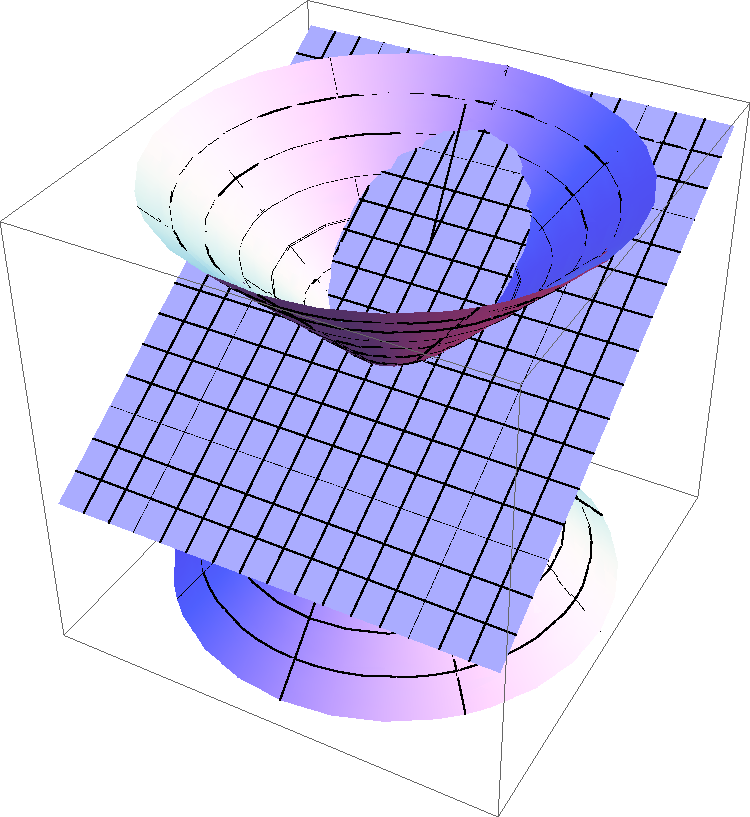
\includegraphics[width=0.47\linewidth,height=0.45\linewidth,clip]{Lightcone_2} %\hspace{0.3cm}
%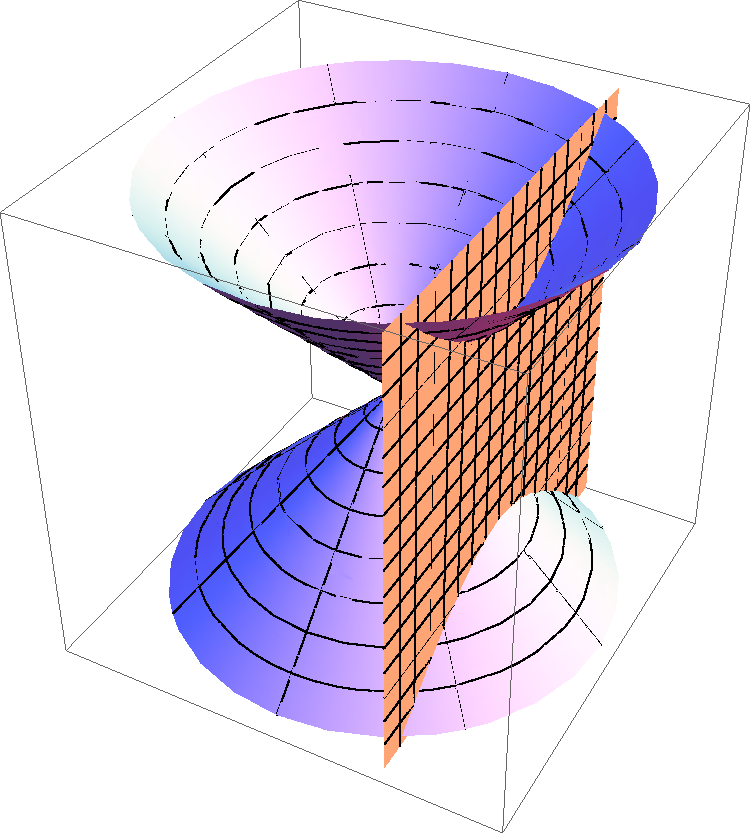
\includegraphics[width=0.5\linewidth,height=0.5\linewidth,clip]{Lightcone_1}
\caption[]{ \label{fig:lightcone}
(links) In zwei Raumdimensionen schneidet die Gleichzeitigkeitsebene
zu einem Beobachter 2 den Lichtkegel in einer Ellipse. Die
gro\ss e Halbachse entspricht dem gesuchten Abstand $A'B'$ 
bzw.\ $B'C'$, die kleine Halbachse ist senkrecht zur
relativen Bewegung und hat daher f\"ur Beobachter 1 und
2 dieselbe L\"ange. Andererseits soll sich f\"ur Beobachter
2 das Licht in alle Richtungen gleich schnell ausbreiten, d.h.\
f\"ur Beobachter 2 haben die gro\ss e und die kleine
Halbachse der Ellipse dieselbe L\"ange. (rechts)
Die Punkte mit einem konstanten Abstand von der
$(x,t)$-Ebene schneiden den Lichtkegel in einer
Hyperbel, d.h.\ alle Punkte auf dieser Hyperbel haben 
von der $(x,t)$-Ebene denselben Abstand.}
\end{figure}


Wir haben oben die relative Skala durch Vergleich mit
einer zweiten Raumdimension, relativ zu der sich zwei
Inertialsysteme nicht bewegen, abgeleitet. Es gibt noch eine
zweite M\"oglichkeit, die sich auch in zwei Dimensionen 
anwenden l\"asst:
Wir integrieren das Vektorfeld, das in jedem Punkt durch
die Richtung der Gleichzeitigkeit erzeugt wird. Dies f\"uhrt auf die
Bedingung\index{Gleichzeitigkeit}
\[    \frac{{\rm d}x}{{\rm d}t} ~=~ \frac{t}{x} 
      \hspace{1cm} {\rm oder} \hspace{1cm}
      t^2 - x^2 ~=~ {\rm const.}~~  . \]
Alle Ereignisse auf einer solchen Hyperbel haben denselben 
Abstand vom Ursprung. Insbesondere gilt
\[    t_{\rm B}^2 - x_{\rm B}^2 ~=~ t_{\rm D}^2  \;, \]
und da $x_{\rm B} =v t_{\rm B}$ folgt
\[    t_{\rm B}^2 - v^2 t_{\rm B}^2 ~=~ t_{\rm D}^2 \]
oder 
\[       t_{\rm D} ~=~ \frac{1}{\sqrt{1-v^2}} t_{\rm B}  \;. \]
Dieses Verfahren setzt voraus, dass Ereignisse mit einem konstanten
Abstand vom Ursprung in gewisser Hinsicht \glqq stetig\grqq\ sind, und da\ss\
wir infinitesimal annehmen k\"onnen, dass solche Ereignisse f\"ur
einen Beobachter, der sich gleichf\"ormig vom Ursprung zu einem dieser
Ereignisse bewegt, lokal gleichzeitig sind.



\begin{thebibliography}{99}
\addcontentsline{toc}{chapter}{Literaturangaben}
\bibitem{Aichelburg} Peter C.\ Aichelburg (Hrsg.); {\it Zeit im 
       Wandel der Zeit}; Verlag Vieweg, Braunschweig, Wiesbaden, 1988.
\bibitem{Born} Max Born; {\it Optik}; Springer-Verlag, Berlin, Heidelberg,
        1972.
\bibitem{Britannica} Encyclopaedia Britannica; 15.th edition, 1988.
\bibitem{Descartes} Ren\'e Descartes; {\it Die Prinzipien der
        Philosophie}; Felix Meiner Verlag, Hamburg, 1992; \"ubersetzt
        von Artur Buchenau.
\bibitem{Einstein1} Albert Einstein; {\it Zur Elektrodynamik bewegter 
        K\"orper}; Annalen der Physik, Leipzig, 17 (1905) 891. 
\bibitem{Helmholtz2} Hermann von Helmholtz; {\em \"Uber Wirbelbewegungen,
        \"Uber Fl\"ussigkeitsbewegungen}, 1858; in Ostwalds Klassiker der 
       exakten Wissenschaften Bd.\ 1; Verlag Harri Deutsch, Frankfurt, 
       1996.                   
\bibitem{Laue} Max von Laue; {\it Geschichte der Physik}; 
         Universit\"ats-Verlag Bonn, 1947.
\bibitem{Lorentz} Hendrik Antoon Lorentz; {\it Electromagnetic phenomena 
         in a system moving with any velocity smaller than that of light}; 
         Proc.\ Acad.\ Sci., Amsterdam, 6 [1904], S.\ 809.
\bibitem{Mittelstaedt} Peter Mittelstaedt; {\it Der Zeitbegriff in der
        Physik}; BI-Wissenschaftsverlag, 1989.        
\bibitem{Mittelstaedt2} Peter Mittelstaedt; {\it Philosophische Probleme
        der modernen Physik}; BI-Wissenschaftsverlag, 1989.        
\bibitem{Newton2} Isaac Newton; {\it \"Uber die Gravitation...};
       Klostermann Texte Philosophie; Vittorio Klostermann, Frankfurt,
      1988; \"ubersetzt von Gernot B\"ohme.
\bibitem{Newton3} Isaac Newton; {\it Optik oder Abhandlung \"uber
      Spiegelungen, Brechungen, Beugungen und Farben des Lichts};
      I., II.\ und III.\ Buch (1704); aus dem Englischen \"ubersetzt
      von W.\ Abendroth; Ostwalds Klassiker der exakten Wissenschaften,
      Verlag Harri Deutsch 1998.   
\bibitem{Pauli} Wolfgang Pauli; {\it Theory of Relativity}; Dover
      Publications, New York, 1981.      
\bibitem{Poincare} Jules Henri Poincar\'e; {\it Sur la dynamique de 
     l'\'electron}, C.R.\ Acad.\ Sci., Paris, 140 (1905) S.~1504; und 
      Rendiconti del Circolo Matematico di Palermo, Bd.~21 (1906) S.~129.
\bibitem{Sexl} Roman U.\ Sexl, Helmuth K.\ Urbantke; {\it Relativit\"at,
      Gruppen, Teilchen}; Springer-Verlag, Wien, New York, 1992.
\bibitem{Simonyi}
      K\'aroly Simonyi; {\it Kulturgeschichte der Physik}; Verlag
       Harri Deutsch, Thun, Frankfurt am Main, 1990.
\end{thebibliography}

\end{document}

\documentclass[german,10pt]{book}     
\usepackage{makeidx}
\usepackage{babel}            % Sprachunterstuetzung
\usepackage{amsmath}          % AMS "Grundpaket"
\usepackage{amssymb,amsfonts,amsthm,amscd} 
\usepackage{mathrsfs}
\usepackage{rotating}
\usepackage{sidecap}
\usepackage{graphicx}
\usepackage{color}
\usepackage{fancybox}
\usepackage{tikz}
\usetikzlibrary{arrows,snakes,backgrounds}
\usepackage{hyperref}
\hypersetup{colorlinks=true,
                    linkcolor=blue,
                    filecolor=magenta,
                    urlcolor=cyan,
                    pdftitle={Overleaf Example},
                    pdfpagemode=FullScreen,}
%\newcommand{\hyperref}[1]{\ref{#1}}
%
\definecolor{Gray}{gray}{0.80}
\DeclareMathSymbol{,}{\mathord}{letters}{"3B}
%
\newcounter{num}
\renewcommand{\thenum}{\arabic{num}}
\newenvironment{anmerkungen}
   {\begin{list}{(\thenum)}{%
   \usecounter{num}%
   \leftmargin0pt
   \itemindent5pt
   \topsep0pt
   \labelwidth0pt}%
   }{\end{list}}
%
\renewcommand{\arraystretch}{1.15}                % in Formeln und Tabellen   
\renewcommand{\baselinestretch}{1.15}                 % 1.15 facher
                                                      % Zeilenabst.
\newcommand{\Anmerkung}[1]{{\begin{footnotesize}#1 \end{footnotesize}}\\[0.2cm]}
\newcommand{\comment}[1]{}
\setlength{\parindent}{0em}           % Nicht einruecken am Anfang der Zeile 

\setlength{\textwidth}{15.4cm}
\setlength{\textheight}{23.0cm}
\setlength{\oddsidemargin}{1.0mm} 
\setlength{\evensidemargin}{-6.5mm}
\setlength{\topmargin}{-10mm} 
\setlength{\headheight}{0mm}
\newcommand{\identity}{{\bf 1}}
%
\newcommand{\vs}{\vspace{0.3cm}}
\newcommand{\noi}{\noindent}
\newcommand{\leer}{}

\newcommand{\engl}[1]{[\textit{#1}]}
\parindent 1.2cm
\sloppy

     \begin{document}   \setcounter{chapter}{2}  

\chapter{Philosophischer Hintergrund der SRT}   %  Kap. 3
\label{chap_Philosophie}

Betrachtet man vor dem Hintergrund der speziellen 
Relativit\"atstheorie das Modell von Lorentz, so  
wirkt die mechanische Kontraktion physikalischer Systeme
und die zeitliche Verz\"ogerung physikalischer Prozesse
bei einer Bewegung relativ zum \"Ather
eher befremdlich. Insbesondere der 
material\-un\-ab\-h\"angige, universelle Verk\"urzungsfaktor $\sqrt{1-(v/c)^2}$ 
erscheint auf den ersten Blick willk\"urlich. Man gewinnt den Eindruck, als ob
eine entsprechende universelle Wechselwirkung zwischen Materie und
\"Ather, die diesen Verk\"urzungsfaktor erkl\"art, nur in einem sehr 
komplizierten und unnat\"urlichen Modell beschrieben werden kann.

Dies ist jedoch nicht der Fall. Im Gegenteil, die
Maxwell-Theorie oder auch unser heutiges Standardmodell sind ebenfalls in 
der Lage, diesen Verk\"urzungsfaktor zu erkl\"aren. Der Unterschied
zwischen der speziellen Relativit\"atstheorie im Sinne von Einstein und der Lorentz'schen
Theorie (\"Ather, Verk\"urzungsfaktor, etc.) erweist sich nur als eine 
Frage der Interpretation. Der mathematische Formalismus ist derselbe und kein
Experiment kann zwischen den beiden Interpretationen unterscheiden. 
Die heute verbreitete Interpretation, nach der die Effekte der speziellen Relativit\"atstheorie
als Folgerung der Geometrie der Minkowski-Raumzeit gedeutet werden, hat den
Vorteil, keine unbeobachtbaren Elemente - die Entit\"at des \"Athers oder ein ausgezeichnetes
Ruhesystem - zu enthalten. Man spricht in diesem Zusammenhang auch gerne
von Ockhams Rasiermesser (Ockham's Razor): Hierbei handelt es sich um ein nach
Wilhelm von Ockham (1288-1347) benanntes Prinzip der Wissenschaftstheorie, wonach
ein Erkl\"arungsmodell m\"oglichst einfach sein sollte, bzw.\ zwischen zwei Modellen dasjenige
den Vorzug hat, das mit weniger Variablen auskommt.   

Andererseits ist es oft von Vorteil, m\"oglichst viele gleichberechtigte Perspektiven auf einen
Sachverhalt zu haben, und es gibt durchaus Situationen, in denen die Lorentz'sche Interpretation
der Relativit\"atstheorie eine intuitivere Vorstellung vermittelt als die Einstein'sche. Daher beginnt
dieser Abschnitt mit einer Beschreibung dieser Sichtweise. 

\section{Eine Kette gekoppelter Pendel}
\label{sec_Kette}

Wir betrachten zun\"achst ein einfaches mechanisches
Modell, in dem die L\"angenma\ss\-st\"abe eine Lorentz-Kontraktion
erfahren, wenn sie sich mit einer Geschwindigkeit
$v$ relativ zu dem absolut ruhenden Bezugssystem bewegen. Auch die
anderen bekannten Beziehungen aus der speziellen Relativit\"atstheorie
wie beispielsweise die Zeitdilatation werden in diesem Modell wiedergegeben.


\begin{figure}[htb]
\begin{picture}(400,100)(0,0)
\multiput(10,10)(20,0){20}{\line(0,1){80}}
\multiput(10,10)(20,0){20}{\circle*{10}}
\multiput(13.2,40)(20,0){19}{\makebox(0,0){${\scriptstyle \vee}$}}
\multiput(18.1,40)(20,0){19}{\makebox(0,0){${\scriptstyle \vee}$}}
\multiput(23.0,40)(20,0){19}{\makebox(0,0){${\scriptstyle \vee}$}}
\multiput(27.9,40)(20,0){19}{\makebox(0,0){${\scriptstyle \vee}$}}
\put(415,50){\vector(0,-1){40}}
\put(420,30){\makebox(0,0){${\scriptstyle g}$}}
\put(170,0){\makebox(0,0){${\scriptstyle i-1}$}}
\put(190,0){\makebox(0,0){${\scriptstyle i}$}}
\put(210,0){\makebox(0,0){${\scriptstyle i+1}$}}
\put(395,60){\makebox(0,0){${\scriptstyle l}$}}
\put(400,10){\makebox(0,0){${\scriptstyle m}$}}
\put(395,40){\makebox(0,0){${\scriptstyle D}$}}
\thicklines
\put(0,90){\line(1,0){400}}
\end{picture}
\caption{\label{fig_Pendel}%
Eine Kette harmonisch gekoppelter Pendel im
Schwerefeld der Erde. Die Pendel k\"onnen senkrecht
zur Darstellungsebene schwingen. Ihr Freiheitsgrad ist der
Auslenkungswinkel relativ zur Senkrechten. Die Pendelkugeln haben eine Masse $m$,
die harmonische Feder zwischen den Pendeln die Federkonstante $D$. Die L\"ange der
Pendel sei $l$ und $g$ sei die Schwerebeschleunigung der Erde.}
\end{figure}


Als physikalisches Modell stelle man sich eine Kette harmonisch gekoppelter
\index{Pendelkette}
Pendel in einem konstanten Gravitationsfeld vor. Die Pendel seien
mit einem Index $i$ durchnummeriert, wobei wir zun\"achst $i$ die
ganzen Zahlen durchlaufen lassen. Der Freiheitsgrad des $i$-ten 
Pendels ist der Winkel $\varphi_i$ relativ zur herabh\"angenden
Ruhelage. Die Wirkung dieses Modells lautet:
\[  S ~=~ \frac{1}{2} \int \! {\rm d} t \sum_i \left[   
       \left( \frac{\partial \varphi_i(t)}{\partial t} \right)^2 -
       D \left[ \varphi_{i+1}(t) -\varphi_i(t) \right]^2 +
       2 g \cos \varphi_i(t)  \right]  \;,    \]
und die zugeh\"orige Bewegungsgleichung des 
$i$-ten Pendels ist:
\begin{equation}
\label{discrete}
  \frac{\partial^2 \varphi_i(t)}{\partial t^2} -         
  D [\varphi_{i+1}(t) - 2 \varphi_i(t) + \varphi_{i-1}(t) ]
  + g \sin \varphi_i ~=~ 0 \;. 
\end{equation}             
Suchen wir nach L\"osungen, bei denen sich die Winkel benachbarter Pendel 
nicht wesentlich unterscheiden, muss $g\ll D$ gelten. 
In diesem Fall k\"onnen wir das diskrete Modell
durch ein kontinuierliches feldtheoretisches Modell mit der Wirkung
\[  S ~=~ \frac{1}{2} \int \! {\rm d} t\, {\rm d} x~ \left[   
        \left( \frac{\partial \varphi(x,t)}{\partial t} \right)^2 -
        \left( \frac{\partial \varphi(x,t)}{\partial x} \right)^2 +
        g \cos \varphi(x,t)  \right]     \]
und den Feldgleichungen 
\begin{equation}
\label{eq_cont}
  \frac{\partial^2 \varphi}{\partial t^2} -         
    \frac{\partial^2 \varphi}{\partial x^2} + g \sin \varphi ~=~ 0 
\end{equation}             
approximieren. Hier wurde $D=1$ gesetzt und der kontinuierliche
Parameter $x$, der den Ort entlang der Aufh\"angung bezeichnet,
ersetzt die Nummerierung der Pendel. Die folgenden \"Uberlegungen
gehen immer von diesem kontinuierlichen Modell aus.
Die Kennzeichnung der Raum-Zeit-Punkte $(x,t)$ bezieht sich jedoch auf 
eine feste, Newton'sche Hinter\-grunds\-raum\-zeit. Daher ist es auch
ganz instruktiv, sich die Kette gekoppelter Pendel vorzustellen,
da in diesem Fall der klare -- Newton'sche -- Charakter von \glqq Raum\grqq\ und
\glqq Zeit\grqq\ deutlicher wird.

Wir wissen, dass die Kontinuumsfeldgleichung (\ref{eq_cont}) invariant
\index{Lorentz-Transformation}
unter Lorentz-Transformationen ist. Eine solche Feststellung ist
zun\"achst keine Aussage \"uber die zugrundeliegende Raum-Zeit-Struktur, 
sondern bezeichnet eine Eigenschaft der 
L\"osungs\-menge der Gleichungen: 
Wenn $\varphi_0(x,t)$ eine L\"osung der Gleichung (\ref{eq_cont}) ist, dann ist 
auch
\begin{equation}
\label{eq_inv}
   \varphi_v(x,t) ~=~
   \varphi_0\left(\,\gamma(v)(x-vt)\:,\:
                \gamma(v) (t-  v x)\, \right)
   ~~~{\rm mit}~~ \gamma(v) = \frac{1}{\sqrt{1-v^2}}
\end{equation}
eine L\"osung dieser Gleichung f\"{u}r beliebiges $-1<v<1$. Solange $g\ll 1$,
bzw.\ der Wert f\"{u}r $v$ so eingeschr\"ankt wird, da{\ss} auch $g\gamma(v)\ll 1$
(in unserer Normierung ist $c=1$), werden die L\"osungen der diskretisierten
Gleichung (\ref{discrete}) durch die L\"osungen der 
Kon\-ti\-nuums\-gleichung angen\"ahert. 
Im Rahmen dieser N\"aherung werden die diskretisierten
L\"osungen daher auch dieselbe Invarianzeigenschaft (\ref{eq_inv}) zeigen. 

Da wir untersuchen wollen, wie sich L\"angenma\ss st\"abe und Uhren
verhalten, wenn man sie gegen das Ruhesystem bewegt, m\"ussen wir
zun\"achst intrinsische \glqq Lineale\grqq\ und \glqq Uhren\grqq\ definieren. Dazu
benutzen wir die besonderen L\"osungen
der Sinus-Gordon-Gleichung: die Soliton-L\"{o}sung und die L\"osung zu
gebundenen Zust\"{a}nden von zwei Solitonen -- die Breather-L\"osungen.
Die genaue Form der L\"osungen spielt f\"ur das Folgende
keine Rolle, wird aber (um wirklich explizit zu sein) angegeben.
Wie wir sehen werden, ist nur die oben erw\"ahnte Invarianz
der L\"osungsmenge von Bedeutung.

\begin{figure}[htbp]
\includegraphics[width=0.47\linewidth,height=0.28\linewidth,clip]{./Bilder_SRT/Soliton_phi} \hspace{0.3cm}
\includegraphics[width=0.47\linewidth,height=0.28\linewidth,clip]{./Bilder_SRT/Soliton_Height}%\\[0.5cm]
%\hspace*{3cm}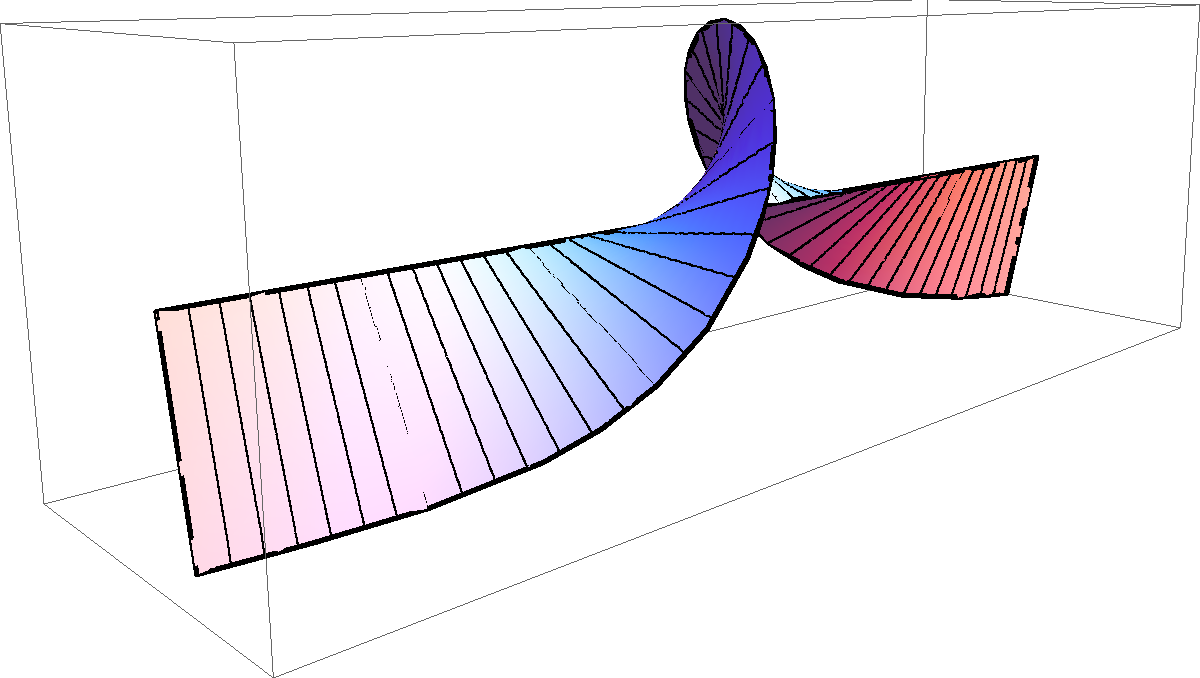
\includegraphics[width=0.5\linewidth,height=0.3\linewidth,clip]{./Bilder_SRT/Soliton_3D}
\caption[]{ \label{fig:Soliton}
Die Soliton-L\"osung: (oben links) Der Auslenkungswinkel $\varphi$ 
als Funktion der Koordinate $x$ entlang der Aufh\"angung,
(oben rechts) die Seitenansicht.}
% (unten) die dreidimensionale Ansicht.}
\end{figure}

Die Soliton-L\"osung entspricht einer Konfiguration, bei der sich die
Pendel in der N\"ahe eines Punktes einmal um ihre Aufh\"angung herumwinden, 
sich anderenfalls aber im Wesentlichen in der
senkrecht herabh\"angenden Ruhelage befinden (siehe Abb.\ \ref{fig:Soliton}). 
Diese L\"osung ist stabil. 
Die statische L\"{o}sung des Kontinuumsmodells ist durch
\index{Soliton}
\begin{equation}
\label{soliton}
      \varphi_0(x) ~=~ 4 \tan^{-1}
      \left( \exp \pm \sqrt{g}(x-x_0) \right) 
\end{equation}
gegeben, wobei die Integrationskonstante $x_0$ die Position
des Solitons angibt, d.h.\ den Punkt, bei dem $\varphi=\pi$. 
Das + Zeichen in (\ref{soliton}) entspricht einer L\"osung, f\"ur die
$\lim_{x\rightarrow -\infty} \varphi(x) \rightarrow 0$ und
$\lim_{x\rightarrow +\infty} \varphi(x) \rightarrow 2\pi$. Das $-$ 
Zeichen beschreibt eine so\-ge\-nann\-te Anti-Soliton-L\"osung mit
$\lim_{x\rightarrow -\infty} \varphi(x) \rightarrow 2\pi$ und
$\lim_{x\rightarrow +\infty} \varphi(x) \rightarrow 0$.
In beiden F\"allen n\"ahern sich die L\"osungen ihrem asymptotischen Wert
f\"ur gro\ss e $|x-x_0|$ exponentiell. Die Reichweite der L\"osung 
entspricht dabei
\begin{equation}
\label{width}
   \Delta L ~=~ 1/\sqrt{g}   \;.
\end{equation}
Diese Gr\"o\ss e ist ein Ma\ss\ f\"ur die halbe Breite des Solitons und
soll uns als L\"angenskala dienen. 

\begin{figure}[htbp]
\includegraphics[width=0.47\linewidth,height=0.28\linewidth,clip]{./Bilder_SRT/Breather_phi} \hspace{0.3cm}
\includegraphics[width=0.47\linewidth,height=0.28\linewidth,clip]{./Bilder_SRT/Breather_Height}%\\[0.5cm]
%\hspace*{3cm}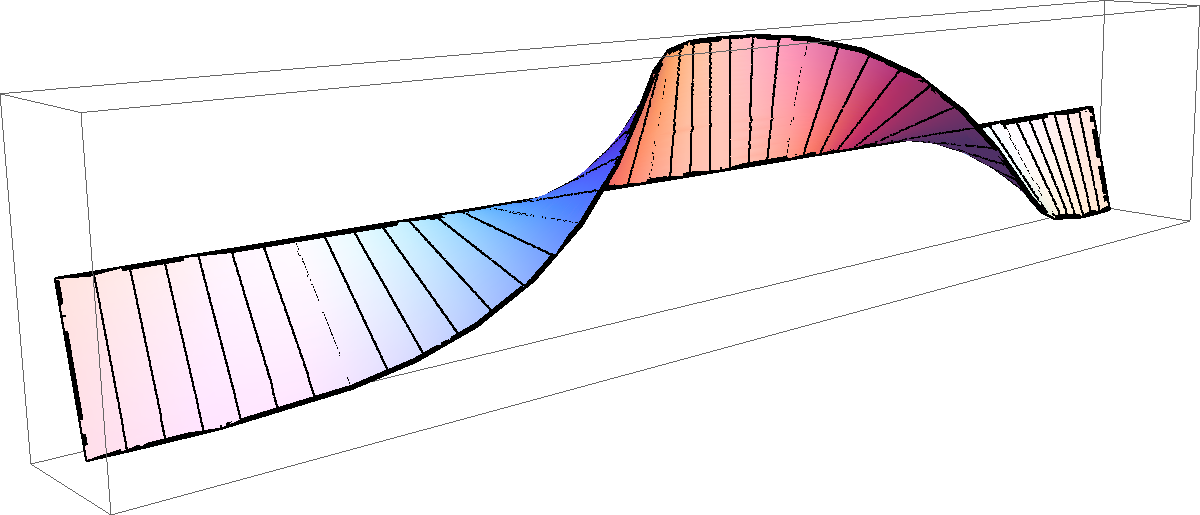
\includegraphics[width=0.5\linewidth,height=0.3\linewidth,clip]{./Bilder_SRT/Breather_3D}
\caption[]{ \label{fig:Breather}
Die Breather-L\"osung: (oben links) Der Auslenkungswinkel $\varphi$ 
als Funktion der Koordinate $x$ entlang der Aufh\"angung im
Augenblick maximaler Auslenkung,
(oben rechts) die Seitenansicht.}
%, (unten) die dreidimensionale Ansicht.}
\end{figure}

Die Sinus-Gordon Theorie besitzt ebenfalls L\"osungen, die gebundenen
Zust\"anden eines Solitons und eines Anti-Solitons entsprechen, die 
sogenannten Breather-L\"osungen (vgl.\ \cite{Lamb}; Darstellung in
Abb.\ \ref{fig:Breather}):
\index{Breather-L\"osung}
\begin{equation}
\label{breather}
    \varphi_0(x,t) ~=~ - 4 \tan^{-1} \left[ \frac{m}{\sqrt{1-m^2}}
    \frac{\sin \sqrt{g(1-m^2)}(t-t_0)}{\cosh m \sqrt{g}(x-x_0)} \right]\;.
\end{equation}
Der Parameter $m$ muss der Bedingung $0<m^2<1$ gen\"ugen, ist ansonsten 
aber beliebig. Die Schwingungsperiode ist
\begin{equation}
\label{time}
     \Delta T ~=~ \frac{2\pi}{\sqrt{g(1-m^2)}}~.
\end{equation}
Diese L\"osung ist metastabil. Es handelt sich um einen gebundenen
Zustand zwi\-schen einem Teilchen und seinem Antiteilchen, und kleine
St\"orungen lassen dieses System in \glqq Photonen\grqq\ zerfallen, d.h.\
einfache Schwingungen der Pendelkette. Der freie
Parameter $m$ h\"angt mit der Bindungsenergie zusammen und legt sowohl die
Amplitude als auch die Periode fest. Zur Festlegung einer Zeitskala
muss daher ein spezieller Wert f\"ur $m$ gew\"ahlt werden. Eine m\"ogliche
Wahl w\"are, dass $\varphi$ zwischen $-\pi$ und $+\pi$ variiert, d.h.\
$m^2=1/2$ oder $\Delta T=\sqrt{8\pi^2/g}$. (Dieser Wert f\"ur $m$ wurde
in Abb.\ \ref{fig:Breather} gew\"ahlt.)
\vspace{0.3cm}

Wir wollen nun untersuchen, wie sich die so definierten L\"angen-
und Zeitma\ss st\"abe transformieren, wenn man sie relativ zum
\glqq \"Ather\grqq, d.h.\ dem durch die Pendel definierten Ruhesystem,
bewegt.
Wir betrachten zun\"achst ein Soliton mit einer Geschwindigkeit
$v$. Diese L\"osung erhalten wir aus der statischen L\"osung nach 
Gleichung (\ref{eq_inv}). Auch die Breite des propagierenden Solitons
l\"asst sich daraus ablesen. 

Die statische L\"osung $\varphi_0(x)$ habe ihr Zentrum bei $x=0$. Dann
bestimmt die Bedingung
\[         \varphi_0(\pm \Delta L) ~=~ \pi \pm \alpha   \]
einen Wert f\"ur $\alpha$, bei dem wir die Breite von $\varphi_0$ messen.
F\"ur die propagierende L\"osung
\[         \varphi_v(x,t) ~=~ \varphi_0(\,\gamma(v)(x-vt)\,) \;,  \]
bewegt sich das Zentrum $x_0(t)$ nach der Gleichung $x_0(t)=vt$. Die
Breite dieser L\"osung ist gleich dem Wert $\Delta L_v$, der der
Bedingung
\[    \varphi_v(x_0(t)\pm \Delta L_v,t) ~=~ \pi \pm \alpha  \]
gen\"ugt. Dies ist offensichtlich der Fall f\"{u}r
\begin{equation}
\label{Lorentz}
        \gamma(v)\, \Delta L_v ~=~ \Delta L ~~~{\rm oder} ~~~
        \Delta L_v ~=~ \sqrt{1-v^2} \Delta L \;.  
\end{equation}
Die Breite der propagierenden L\"{o}sung ist daher um einen Faktor
$1/\gamma(v)$ kontrahiert. Diese \glqq Lorentz-Kontraktion\grqq\ kann von
\index{Lorentz-Fitzgerald-Kontraktion}
einem au\ss enstehenden Beobachter, der sieht, wie sich die Solitonen
entlang der Pendelkette ausbreiten, tats\"achlich wahrgenommen werden.

\begin{figure}[htbp]
\includegraphics[width=0.47\linewidth,height=0.28\linewidth,clip]{./Bilder_SRT/Soliton_Height} \hspace{0.3cm}
\includegraphics[width=0.47\linewidth,height=0.28\linewidth,clip]{./Bilder_SRT/Soliton_v09}
\begin{picture}(0,0)(0,0)
\thicklines
\put(-90,100){\vector(1,0){20}}
\put(-80,110){\makebox(0,0){$v=0{,}9$}}
\put(-280,110){\makebox(0,0){$v=0$}}
\end{picture}
\caption[]{ \label{fig:Soliton_v09}
Die Soliton-L\"osung in Bewegung: (links) Die ruhende 
Soliton-L\"osung aus Abb.\ \ref{fig:Soliton}, (rechts) 
die zugeh\"orige transformierte L\"osung zu einer 
Geschwindigkeit $v=0{,}9$.}
\end{figure}

Auch die Dilatation der Schwingungsperiode des gebundenen Zustands l\"asst
sich leicht herleiten. In Ruhe gilt f\"{u}r die Breather-L\"osung:
\[      \varphi_0^b(x,t) ~=~ \varphi_0^b(x,t+\Delta T) \;. \]
Die zugeh\"orige propagierende L\"osung erf\"ullt
\[   \varphi_v^b(x,t) ~=~ \varphi_v^b(x+v\Delta T_v, t+\Delta T_v) \;. \]
Da
\[   \varphi_v^b(x,t) ~=~
     \varphi_0^b \left(\,\gamma(v)(x-vt)\:,\:\gamma(v)(t-vx)\,\right)  \]
erhalten wir
\[   \gamma(v) \left( t+ \Delta T_v - v
     \left( x + v \Delta T_v \right) \right) ~=~
     \gamma(v) \left(t-v x \right) +
     \gamma(v) \left( 1-v^2\right) \Delta T_v \]
und somit:
\begin{equation}
\label{dilation}
      \Delta T ~=~ \gamma(v) \left(1-v^2 \right) \Delta T_v
      ~~~{\rm oder}~~~
      \Delta T_v ~=~ \frac{1}{\sqrt{1-v^2}} \Delta T \;.
\end{equation}
Die Schwingungsdauer eines sich bewegenden gebundenen Zustands ist
also tats\"achlich um einen Faktor $\gamma(v)$ im Vergleich zum ruhenden
Zustand verl\"angert.

Solitonen und gebundene Zust\"{a}nde von Solitonen k\"onnen an einem
festen Ende der Kette ohne Energieverlust reflektiert werden. Durch
eine solche experimentelle Anordnung kann man das 
\index{Zwillingsparadoxon}
\glqq Zwillingsparadoxon\grqq\ aufzeigen (vgl.\ Abschnitt \ref{chap_Zwilling}): 
Ein gebundener Zustand, der
sich entlang der Kette bewegt und nach einer Reflektion am Ende
der Kette zur\"uckkehrt, hat weniger Schwingungen ausgef\"uhrt, als ein
ruhender gebundener Zustand. Offensichtlich kann dieser Effekt
nicht der \glqq Beschleunigung\grqq\ am Ende der Kette
zugeschrieben werden.

\section{Von der \"Atherhypothese zur Relativit\"atstheorie}

Zun\"achst hat es vielleicht den Anschein, als ob das oben diskutierte
Modell der harmonisch gekoppelten Pendel sehr speziell sei. 
Hinsichtlich der Existenz von Soliton- und Breather-L\"osung mag das
richtig sein, nicht aber hinsichtlich der Tatsache, dass
dieses Modell den richtigen Verk\"urzungsfaktor und die richtige
Zeitdilatation liefert. Das einzige, was wir zur Herleitung dieser
Faktoren benutzt haben, ist die Lorentz-Invarianz der Feldgleichungen.
{\em Jede Lorentz-invariante Feldgleichung hat somit die Eigenschaft, dass
ihre L\"osungen, die eine L\"angen- oder Zeitskala definieren, sich genau
so transformieren, dass die bewegten Ma\ss st\"abe bzw.\ Uhren 
mit dem Lorentz'schen Verk\"urzungs- bzw.\ Dilatationsfaktor
multipliziert werden.}

Insbesondere haben auch die Maxwell-Gleichungen diese Eigenschaft.
Genau das hatte Lorentz gezeigt, wobei er allerdings noch die
falschen Transformationsgesetze f\"ur die Ladungen und Str\"ome
verwendet hatte. Diesen Fehler hat Poincar\'e korrigiert. Unter der 
Annahme, dass auf atomarer Ebene die 
Materie, und damit auch L\"angenma\ss st\"abe, durch die 
elektromagnetische Wechselwirkung zusammengehalten 
wird, war daher
die Lorentz-Kontraktion nicht nur plausibel sondern sogar eine
Folgerung aus den Maxwell-Gleichungen. 

Vor diesem Hintergrund k\"onnen wir auch den \"Ubergang
von der Lorentz'schen Sichtweise zur 
Einstein'schen Sichtweise und der 
speziellen Relativit\"atstheorie leichter nachvollziehen. 
Aus der Lorentz-Invarianz der fundamentalen Gleichungen
folgen ja nicht nur die Lorentz-Kontraktion und die Zeitdilatation,
sondern s\"amtliche Ph\"anomene, die sich im Rahmen der speziellen
Relativit\"atstheorie erkl\"aren lassen.

Oftmals wird behauptet, der \"Ubergang zur 
Sichtweise der speziellen Relativit\"atstheorie 
best\"unde in einer Neuinterpretation von 
\glqq Raum\grqq\ und \glqq Zeit\grqq.
Doch \"uber Raum und Zeit als abstrakte Entit\"aten 
k\"onnen wir eigentlich nichts sagen. In der Physik
interessieren wir uns nur f\"ur r\"aumliche und zeitliche
{\em Distanzen}, und diese Distanzen messen wir mir
physikalischen Instrumenten -- L\"angenma\ss st\"aben
und Uhren --, die selbst den physikalischen Gesetzen
unterliegen. 

Bisher bezog sich das Symbol $x$ auf 
eine Koordinate im Ruhesystem des
\"Athers -- im obigen Modell war dies das 
Ruhesystem der Pendelaufh\"angung. 
Dies entspricht dem \glqq Lineal\grqq\ eines 
externen Beobachters, der au\ss erhalb
unserer Welt steht und alles mit 
seinen Ma\ss st\"aben ausmessen kann -- 
wie wir bei den gekoppelten Pendeln. Entsprechend 
bezog sich auch das Symbol $t$ auf die Uhr eines externen Beobachters. Wir als
externe Beobachter k\"onnen die L\"angenkontraktion der Solitonen 
nachweisen, indem wir einfach ein \glqq externes\grqq\ 
Lineal neben das Soliton halten. Ebenso 
k\"onnen wir den propagierenden gebundenen Zustand beobachten und die 
Dilatation in der Schwingungsperiode 
mit unserer externen Uhr vergleichen. F\"ur uns als externe
Beobachter sind Raum (gemessen entlang der Pendelkette) und Zeit absolut. 
$c=1$ (die Geschwindigkeit von Wellen bzw.\ kleinen St\"orungen entlang der
Kette) ist f\"ur uns keine obere Grenzgeschwindigkeit, und wenn wir uns
entlang der Kette bewegen, ist die Ausbreitungsgeschwindigkeit einer
St\"orung entlang der Kette (das entspricht der Ausbreitung des Lichts)
in unserem System f\"{u}r die Vorw\"arts- und
R\"uckw\"artsrichtung verschieden: Das Ruhesystem der Pendelkette ist ein
ausgezeichnetes System.

Stellen wir uns nun jedoch (1+1)-dimensionale Wesen vor, die in dieser
\glqq Soliton-Welt\grqq\ leben. Ihnen stehen nur die Solitonen bzw.\ andere 
L\"osungen ihrer \glqq universellen Be\-we\-gungs\-glei\-chungen\grqq\ 
als L\"angen- und Zeitma\ss st\"abe zur Verf\"{u}gung. Sie werden daher
die Breite eines Solitons und die Schwingungsdauer der Breather-L\"osung
als L\"angen- und Zeitma\ss stab zur Beschreibung der physikalischen
Ph\"anomene benutzen. Doch wenn sie ein bewegtes Soliton mit
der Breite eines anderen bewegten Solitions vergleichen, \glqq messen\grqq\
sie keine Verk\"urzung, entsprechend messen sie auch mit
bewegten Breather-L\"osungen keine Ver\"anderungen in der
Zeitskala eines entsprechend bewegten Systems. Erst wenn sie
die Breite oder Zeitskalen von bewegten Systemen mit denen
von anders bewegten oder ruhenden Systemen vergleichen,
messen sie Unterschiede.

Der \"Ubergang zur Minkowski-Welt erfolgt gerade 
dadurch, dass die externen L\"angen- und Zeitma\ss st\"abe 
durch interne L\"angen- und Zeitma\ss st\"abe, die
denselben physikalischen Gesetzen unterliegen,
ersetzt werden. Es ist der \"Ubergang von
einer externen zu einer internen Perspektive.
Die zugrundeliegende diskrete Struktur 
und damit das ausgezeichnete Ruhesystem (der \glqq \"Ather\grqq) zeigen sich 
erst, wenn $v$ so gro\ss\ wird, dass die Brei\-te der Solitonen mit der 
Gr\"o\ss enordnung des 
Pendelabstands (bzw.\ der Gitterstruktur) vergleichbar wird. Ist die
fundamentale Theorie eine Kontinuumstheorie, 
so tritt der \glqq \"Ather\grqq\ 
f\"ur einen internen Beobachter \"uberhaupt nicht in Erscheinung.

Wenn wir von der Lorentz-Invarianz bzw.\ allgemeiner Poincar\'e-Invarianz
\index{Lorentz-Invarianz}
der Raum-Zeit sprechen, sollten wir eigentlich zwei Schritte bzw.\
Aspekte unterscheiden. Wir haben oben die Invarianzeigenschaft der
Bewegungsgleichungen als eine Eigenschaft der L\"osungsmenge dieser
Gleichungen interpretiert: Mit jeder L\"osung
$\varphi(x)$ ist auch $\varphi^{(\Lambda,a)}(x)=\varphi(\Lambda x -a)$  
eine L\"osung der Bewegungsgleichung. Gibt es nun ausgezeichnete
L\"osungen, die L\"angenma\ss st\"abe oder Uhren definieren, so bedeutet
diese Invarianz, dass bewegte L\"angenma\ss st\"abe k\"urzer, bewegte
Uhren langsamer erscheinen. Dies gilt zun\"achst bez\"uglich der
festen \glqq Hintergrunds-Raum-Zeit\grqq. Diesen Schritt hatte auch Lorentz
erkannt. Der wesentliche zweite Schritt aber blieb Einstein vorbehalten.
Er erkannte n\"amlich, dass die Poincar\'e-Invarianz einer Gleichung
auch bedeutet, dass bez\"uglich der intrinsischen Ma\ss st\"abe
das Relativit\"atsprinzip gilt und damit kein Inertialsystem
mehr ausgezeichnet ist. 

Statt die Lorentz-Invarianz der Gleichungen als Eigenschaft der
L\"osungsmenge anzusehen, was beispielsweise auch f\"ur die diskretisierte
Pendelkette einfach zu interpretieren war, k\"onnen wir die 
Lorentz-Invarianz auch als eine Freiheit der Koordinatenwahl auffassen.
Wenn wir n\"amlich die Raum- und Zeitkoordinaten einer 
Lorentz-Transformation unterwerfen, f\"ur eine Raumdimension somit
die Ersetzung
\begin{equation}
\label{LT}
   x \rightarrow x' ~=~ \frac{x - vt}{\sqrt{1-\beta^2}}  
    \hspace{0.5cm} {\rm und} ~~
    t \rightarrow t' ~=~ \frac{t - \frac{v}{c^2}x}{\sqrt{1-\beta^2}}
    \hspace{1cm} \left(\beta = \frac{v}{c} \right)  
\end{equation}    
vornehmen,
dann bleiben die Feldgleichungen unver\"andert. Ordnen wir nun die
Koordinaten $(x,t)$ bzw.\ $(x',t')$ jeweils Beobachtern zu, deren Weltlinie 
durch $x=0$ bzw.\ $x'=0$ und deren 
\glqq gleichzeitige Ereignisse\grqq\ 
durch die Bedingungen $t=$const.\ bzw.\ $t'=$const.\ definiert sind,
dann bedeutet die Invarianz der Feldgleichungen, dass beide Beobachter
dieselbe Physik sehen, d.h., es gilt das Relativit\"atsprinzip.  

Die Lorentz-Invarianz der Bewegungsgleichungen k\"onnen wir
offensichtlich physikalisch auf zwei vollkommen unterschiedliche Weisen
interpretieren. Einmal als Eigenschaft der L\"osungsmenge, die es uns
erlaubt, aus bestimmten L\"osungen andere zu gewinnen. Diese 
Interpretation bezieht alles auf einen festen Satz von Koordinaten $(x,t)$
(vgl.~(\ref{eq_inv})), der als das Koordinatensystem eines ausgezeichneten
Ruhesystems interpretiert werden kann. Bez\"uglich dieser Koordinaten
beobachten wir die Lorentz-Kontraktion und die Zeitdilatation. 

Die andere Interpretation impliziert das Relativit\"atsprinzip. Wenn
sich zwei Beobachter relativ zueinander mit einer konstanten 
Geschwindigkeit $v$ bewegen, k\"onnen sie unterschiedliche
Koordinatensysteme verwenden, in denen sie sich jeweils im
Ursprung (und damit in Ruhe) befinden. Jeder verwendet zur
Angabe von r\"aumlichen und zeitlichen Distanzen Werte, die mit 
Instrumenten in seinem System gemessen wurden. 
Die von den beiden Beobachtern verwendeten 
Koordinaten h\"angen \"uber die Gleichungen
(\ref{LT}) miteinander zusammen. In diesem Fall erfahren beide
Beobachter dieselbe Physik. In dieser Interpretation gibt es kein
ausgezeichnetes Ruhesystem -- der \"Ather ist verschwunden. 
Der Preis ist eine neue Vorstellung von Gleichzeitigkeit. Dieser letzte
Schritt zeichnete Einstein vor Lorentz und Poincar\'e aus. 
      
\section{Die Synchronisation von Uhren}
\label{sec_Synch}

Ein ungewohnter (und in manchen Kreisen immer noch umstrittener) Aspekt der speziellen
Relativit\"atstheorie ist ihr Konzept von Gleichzeitigkeit. 
Dabei wird\index{Gleichzeitigkeit}
oft vergessen, dass es sich bei der Behauptung, zwei 
Ereignisse seien gleichzeitig, nicht um eine
\glqq faktische\grqq\ Aussagen handelt, sondern 
eher um eine Konvention.\footnote{Versteht man unter \glqq faktisch\grqq, dass
sich alle Beobachter unabhh\"angig von ihrem Bezugssystem in einer Aussage
einig sind, so ist die Gleichzeitigkeit in der Newton'schen Physik faktisch, in der
Relativit\"atstheorie jedoch nicht.}
Ob zwei Ereignisse f\"ur ein gegebenes Inertialsys\-tem gleichzeitig
stattfinden oder
nicht, k\"onnen wir experimentell nur entscheiden, wenn wir eine
Vorschrift angeben, was wir unter \glqq gleichzeitig\grqq\ verstehen
wollen. Diese Vorschrift wird letztendlich darin bestehen, dass wir
zwei Ereignisse als gleichzeitig ansehen, wenn die Uhren
am jeweiligen Ort dieser Ereignisse dieselbe Zeit anzeigen, womit wir das
Problem auf die Synchronisation von Uhren an verschiedenen
Orten (aber im selben Inertialsystem) reduzieren haben. 
Die einzige Einschr\"ankung ist, dass zwei gleichzeitige 
Ereignisse $A$ und $B$ {\em nicht} in einer kausalen Abh\"angigkeit stehen 
sollten. Grunds\"atzlich k\"onnen wir
eine beliebige raumartige Hyperfl\"ache als gleichzeitig {\em definieren}.

Die folgenden \"Uberlegungen gelten f\"ur den flachen Minkowski-Raum.
Wir konzentrieren uns ausschlie\ss lich auf den Aspekt der
Synchronisation\index{Synchronisation von Uhren} 
von Uhren f\"ur ein gegebenes Inertialsystem. Eine
ausf\"uhrlichere Darstellung dieser Problematik findet man bei 
Mittelstaedt \cite{Mittelstaedt} sowie in den beiden Abhandlungen
{\em Philosophie der Raum-Zeit-Lehre} \cite{Reichenbach1} und 
{\em Axiomatik der relativistischen Raum-Zeit-Lehre} \cite{Reichenbach2}
von Hans Reichenbach\index{Reichenbach, Hans} 
(Hans Friedrich Herbert G\"unther Reichenbach,
{\em geb.\ 26.9.1891 in Hamburg; gest.\ 9.4.1953 in Los Angeles}). 

\subsection{Synchronisation durch Lichtsignale}

Zun\"achst ist es recht hilfreich, sich bei der operationalen
Definition von Gleichzeitigkeit auf ein 
allgemeines Verfahren zu beschr\"anken, das allerdings
noch keine Einschr\"ankung an die M\"oglichkeiten darstellt. 
Wir wollen Uhren durch
Austausch von Lichtsignalen synchronisieren. Beobachter $A$ sendet zum
Zeitpunkt $t_1$ ein Lichtsignal aus. Dieses wird von Beobachter $B$
reflektiert und erreicht Beobachter $A$ zum Zeitpunkt $t_2$. Bezeichnen
wir den Zeitpunkt des Ereignisses der Reflektion des Lichtstrahls bei
Beobachter $B$ mit $t$, so m\"ochte Beobachter
$A$ nun definieren, welches Ereignis auf seiner Weltlinie zu
dem Moment der Reflektion des Lichtstrahls bei Beobachter $B$ gleichzeitig
war, d.h.\ dem Zeitpunkt $t$ entspricht. Die einzige Einschr\"ankung
liefert dabei die Forderung der Kausalit\"at: $t_1 < t < t_2$. Beobachter
$A$ definiert nun:
\[      t ~=~ t_1 + \epsilon(A,B) (t_2 - t_1)     \]
mit 
\[         0 < \epsilon(A,B) < 1  \;.   \]
(Der Einfachheit halber soll das Synchronisierungsverfahren nicht von
der Zeit abh\"angen, d.h.\ $\epsilon(A,B)$ h\"angt nicht zus\"atzlich
noch von $t$ bzw.\ $t_1$ ab.)   

\begin{SCfigure}[50][htb]
\begin{picture}(120,200)(0,0)
\put(20,20){\line(0,1){180}}
\put(80,20){\line(0,1){180}}
\put(20,50){\line(1,1){60}}
\put(20,170){\line(1,-1){60}}
\put(20,80){\line(2,1){60}}
\put(20,10){\makebox{$A$}}
\put(80,10){\makebox{$B$}}
\put(50,0){\makebox{(a)}}
\put(10,50){\makebox{$t_1$}}
\put(10,170){\makebox{$t_2$}}
\put(6,78){\makebox{$x_A$}}
\put(84,108){\makebox{$x_B$}}
\end{picture}
%
\begin{picture}(100,200)(0,0)
\put(20,20){\line(0,1){180}}
\put(80,20){\line(0,1){180}}
\put(20,70){\line(1,1){60}}
\put(20,190){\line(1,-1){60}}
\put(20,100){\line(2,1){60}}
\put(20,100){\line(1,1){60}}
\put(20,100){\line(1,-1){60}}
\put(20,10){\makebox{$A$}}
\put(80,10){\makebox{$B$}}
\put(50,0){\makebox{(b)}}
\put(10,70){\makebox{$t_1$}}
\put(10,190){\makebox{$t_2$}}
\put(7,98){\makebox{$x_A$}}
\put(84,128){\makebox{$x_B$}}
\put(84,40){\makebox{$t'_1$}}
\put(84,160){\makebox{$t'_2$}}
\end{picture}
\caption{\label{figsyn}%
Synchronisation von Uhren durch Lichtstrahlen. Die senkrechten Linien
entsprechen den Weltlinien der Beobachter $A$ und $B$, die zueinander
einen konstanten Abstand halten. (a) Zum Zeitpunkt $t_1$ sendet $A$ ein
Lichtsignal aus, das von $B$ im Ereignis $x_B$ reflektiert wird und
bei $t_2$ wieder Beobachter $A$ erreicht. Durch Vorgabe von $\epsilon_A$
konstruiert $A$ das Ereignis $x_A$, das zu $x_B$ gleichzeitig ist.
(b) Soll die Gleichzeitigkeit der Ereignisse $x_A$ und $x_B$ auch f\"ur
Beobachter $B$ gelten, so muss er sein Verfahren zur Bestimmung der
Gleichzeitigkeit (ausgedr\"uckt durch $\epsilon_B$) so w\"ahlen, 
dass $\epsilon_B=1-\epsilon_A$.} 
\end{SCfigure}

Zun\"achst kann man sich leicht \"uberzeugen, dass durch geeignete 
Wahl von $\epsilon$ tats\"achlich je zwei raumartige Ereignisse $x_A$ und
$x_B$ auf der Weltlinie von $A$ und $B$ als gleichzeitig 
definiert werden k\"onnen (vgl.\ Abb.~\ref{figsyn}). 
Dieses Verfahren bildet daher keine Einschr\"ankung der Allgemeinheit. 
Damit die Hyperfl\"ache der zu $x_A$ gleichzeitigen Ereignisse eine
raumartige Hyperfl\"ache ist, m\"ussen die Richtungsableitungen der 
Funktion $\epsilon(A,B)$ (aufgefasst als eine Funktion von $B$) noch
durch eine Konstante (bei unserer Definition der Lichtgeschwindigkeit
ist diese Konstante 1) beschr\"ankt sein. Durch geeignete Forderungen
an die Funktion $\epsilon$ erh\"alt man verschiedene 
Synchronisationsverfahren.

\subsection{Die Einstein-Synchronisation}

Eine sehr allgemeine Forderung an die Gleichzeitigkeit von Ereignissen
\index{Symmetrie der Gleichzeitigkeit}
ist die Symmetrieforderung: Wenn f\"ur einen Beobachter $A$ das 
Ereignis $x_B$ auf der Weltlinie eines Beobachters $B$ gleichzeitig zu
dem Ereignis $x_A$ auf seiner Weltlinie ist, dann soll umgekehrt auch
f\"ur den Beobachter $B$ das Ereignis $x_A$ gleichzeitig zu $x_B$ sein.
Anhand der Abbildung \ref{figsyn}(b) kann man sich leicht \"uberzeugen,
dass diese Forderung gleichbedeutend mit der Bedingung
\[          \epsilon(A,B) ~=~ 1 - \epsilon(B,A)      \]
ist. 

Eine weitere allgemeine Forderung ergibt sich aus der Homogenit\"at des
\index{Homogenit\"at des Raumes}
Raumes. Wir verlangen, dass sich die Funktion $\epsilon(A,B)$ nicht
\"andert, wenn wir die beiden Beobachter $A$ und $B$ um {\em denselben}
(r\"aumlichen) Vektor verschieben. Symbolisch ausgedr\"uckt:
\[     \epsilon(A+\vec{a},B+\vec{a}) ~=~ \epsilon(A,B)     \;.  \]
Dies bedeutet, dass $\epsilon(A,B)$ nur noch von der r\"aumlichen 
Richtung abh\"angen kann, unter der der Beobachter $B$ von $A$ aus gesehen
wird. Innerhalb einer Halbebene, die die Weltlinie von $A$
als Rand hat, ist $\epsilon$ konstant. Auch diese Forderung verlangen
wir allgemein.

Nun kommen wir zu einer speziellen Forderung, die sich aus der Konstanz
der Lichtgeschwindigkeit ergibt. Da die Lichtgeschwindigkeit f\"ur jeden
Beobachter und f\"ur jede Richtung dieselbe sein soll, k\"onnen wir
zus\"atzlich noch Isotropie 
\index{Isotropie des Raumes}
unserer Gleichzeitigkeitsdefinition verlangen.
$\epsilon$ soll also auch nicht mehr von der r\"aumlichen Richtung 
abh\"angen, unter der $B$ von $A$ aus gesehen wird. In diesem Fall 
gilt
\[       \epsilon(A,B) ~=~ {\rm const}    \;.  \]
Zusammen mit der ersten Forderung der Symmetrie folgt sofort:
\[       \epsilon ~=~ \frac{1}{2}  \;.   \]
Die aus diesem Wert f\"ur $\epsilon$ folgende Synchronisation von
Uhren bezeichnet man als\index{Einstein-Synchronisation} 
Einstein-Synchronisation. 

Das zweite Axiom der speziellen Relativit\"atstheorie - die Konstanz
der Lichtgeschwindigkeit - f\"uhrt uns somit schon zur Festlegung der
Gleichzeitigkeitsvorschrift. Das erste Axiom - 
das Relativit\"atsprinzip\index{Relativit\"atsprinzip} -
geht indirekt in diese Festlegung ein, da wir die Konstanz der 
Lichtgeschwindigkeit und somit die Isotropie der
Synchronisationsvorschrift f\"ur jedes Inertialsystem verlangt haben. 
  
\subsection{Synchronisation mit der \"Atherhypothese}

Wir haben aus der Lorentz-Invarianz der universellen Bewegungsgleichungen
geschlossen, dass die spezielle Relativit\"atstheorie in der 
Formulierung von Einstein \"aquivalent zur Lorentz-Theorie ist, d.h.\
zu einer Theorie mit \"Atherhypothese und Lorentz-Kon\-traktion der
L\"angenskalen. Es sollte daher nicht \"uberraschen, wenn es eine
Synchronisationsvorschrift gibt, die auf die Lorentz-Theorie f\"uhrt.

\begin{figure}[ht]
\begin{picture}(360,200)(0,0)
\put(30,120){\vector(1,0){120}}
\put(80,10){\vector(0,1){170}}
\put(30,20){\line(1,2){80}}
\thicklines
\put(40,40){\line(1,1){80}}
\put(120,120){\line(-1,1){27}}
\thinlines
\put(80,120){\makebox(0,0){{\footnotesize $\bullet$}}}
\put(120,120){\makebox(0,0){{\footnotesize $\bullet$}}}
\put(40,40){\makebox(0,0){{\footnotesize $\bullet$}}}
\put(93,147){\makebox(0,0){{\footnotesize $\bullet$}}}
\put(75,125){\makebox(0,0){$O$}}
\put(32,40){\makebox(0,0){$A$}}
\put(87,150){\makebox(0,0){$B$}}
\put(123,128){\makebox(0,0){$C$}}
\put(75,180){\makebox(0,0){$t$}}
\put(150,115){\makebox(0,0){$x$}}
\put(100,10){\makebox(0,0){(a)}}
%
\put(210,120){\vector(1,0){120}}
\put(260,10){\vector(0,1){170}}
\put(210,20){\line(1,2){80}}
\put(220,80){\line(2,1){100}}
\thicklines
\put(220,40){\line(1,1){80}}
\put(300,120){\line(-1,1){27}}
\thinlines
\put(246.5,93){\makebox(0,0){{\footnotesize $\bullet$}}}
\put(300,120){\makebox(0,0){{\footnotesize $\bullet$}}}
\put(220,40){\makebox(0,0){{\footnotesize $\bullet$}}}
\put(273,147){\makebox(0,0){{\footnotesize $\bullet$}}}
\put(255,125){\makebox(0,0){$O$}}
\put(212,40){\makebox(0,0){$A$}}
\put(267,150){\makebox(0,0){$B$}}
\put(303,128){\makebox(0,0){$C$}}
\put(240,97){\makebox(0,0){$D$}}
\put(255,180){\makebox(0,0){$t$}}
\put(330,115){\makebox(0,0){$x$}}
\put(280,10){\makebox(0,0){(b)}}
\end{picture}
\caption{\label{figuhr}%
\"Ather- und Einstein-Synchronisation. In Teil (a) rekonstruiert der
Beobachter auf der Weltlinie $AB$ das Ereignis $O$ als gleichzeitig zum
Ereignis $C$. Seine Synchronisationsvorschrift h\"angt von der 
Geschwindigkeit $v$ relativ zu dem ausgezeichneteten Ruhesystem ab.
Dabei gilt f\"ur das Verh\"altnis $(AO)/(AB)=(1+v)/2$. 
In Abbildung (b) wird nach der Einstein-Synchronisation aus denselben
Lichtsignalen das Ereignis $D$ als zu $C$ gleichzeitig rekonstruiert.}
\end{figure}

Auch mit \"Atherhypothese verlangen wir von der Gleichzeitigkeit von
\index{Aetherhypothese@\"Atherhypothese}
Ereignissen Symmetrie und Homogenit\"at des Raumes. Was wir jedoch
nicht mehr verlangen k\"onnen, ist die allgemein g\"ultige Isotropie
der Synchronisationsvorschrift. F\"ur ein System, das sich relativ zum
\"Ather mit einer Geschwindigkeit $\vec{v}$ bewegt, wird die
Synchronisationsvorschrift von der Richtung relativ zu $\vec{v}$
abh\"angen. Allgemein wird also nun gelten:
\[         \epsilon(A,B) ~=~ \epsilon(\vec{v};A,B)   \;.   \]
Lediglich f\"ur das ausgezeichnete Inertialsystem, das dem
Ruhesystem des \"Athers entspricht, ist die Lichtgeschwindigkeit in
alle Richtungen dieselbe und somit das Synchronisationsverfahren
symmetrisch:
\[       \epsilon(\vec{v}=0;A,B) ~=~ \frac{1}{2}   \;.   \]
Bewegt sich das Inertialsystem der Beobachter $A$ und $B$ relativ
zum \"Ather mit der Geschwindigkeit $\vec{v}$, so gilt 
(vgl.\ Abb.~\ref{figuhr})
\[      \epsilon(\vec{v};A,B) ~=~ \frac{1}{2} 
        \left( 1 + \frac{|\vec{v}|}{c}\cos \alpha \right)  \;, \]
wobei $\alpha$ der Relativwinkel zwischen der Richtung von $\vec{v}$
und der Halbebene ist, die durch die Weltlinie
von $A$ begrenzt wird und die Weltlinie von $B$ enth\"alt.

Der Vorteil dieses Verfahrens ist, dass Gleichzeitigkeit nun
ein absoluter Begriff wird. Sind zwei Ereignisse $x_A$ und $x_B$
f\"ur einen Beobachter $A$ gleichzeitig, so sind sie es auch f\"ur
alle anderen Beobachter, unabh\"angig von deren Bewegungszustand.
 
Der Nachteil dieses Verfahrens ist jedoch, dass wir das Ruhesystem
des \"Athers nicht kennen. Wir m\"ussen also willk\"urlich ein System
auszeichnen, das wir als Ruhesys\-tem definieren, beispielsweise das
System des Schwerpunkts der in unserem Universum beobachtbaren Massen
oder das Ruhe\-sys\-tem relativ zur Hintergrundstrahlung. (Es ist nicht
selbstverst\"andlich, dass diese beiden Sys\-teme identisch sind.)
Wegen der Geschwindigkeitsabh\"angigkeit des Synchronisationsverfahrens
gilt das Relativit\"atsprinzip nicht mehr. Die Lichtgeschwindigkeit
ist nur im Ruhesystem des \"Athers richtungs\-un\-ab\-h\"angig konstant.

Das Relativit\"atsprinzip gilt jedoch in einer anderen Form:
Wir k\"onnen jedes beliebige Inertialsystem als Ruhesystem definieren
und die Synchronisation der Uhren auf dieses System beziehen. Die
physikalischen Gesetze bleiben dieselben. Hier liegt der physikalisch
unbefriedigende Aspekt dieses Synchronisierungsverfahrens. Wir brechen
die Symmetrie, die sich im Relativit\"atsprinzip ausdr\"uckt,
{\em per Hand}, indem wir ein Inertialsystem auszeichnen. Umgekehrt
tr\"agt die Einstein-Synchronisation dem Relativit\"atsprinzip Rechnung.
Kein Inertialsystem wird durch dieses Verfahren ausgezeichnet. Der
Preis ist allerdings die Relativit\"at der Gleichzeitigkeit.

Unter bestimmten Unst\"anden ist es jedoch sinnvoll, eine
Synchronisation zu w\"ahlen, die der Lorentz'schen Sichtweise
n\"aher ist als der Einstein'schen. Beispielsweise k\"onnte man
die Lorentz'sche Sichtweise so interpretieren, dass iregendwo in der Mitte
unseres Universums eine riesige Uhr steht, und das, was diese Uhr anzeigt,
ist die \glqq wahre\grqq\ Zeit. Alle anderen Systeme m\"ussen ihre Zeit auf
diese wahre Zeit umrechnen. Dieses Verfahren wird in abgewandelter Form
beispielsweise bei der Zeitsynchronisation des GPS-Satellitensystems verwendet.
Die \glqq riesige Uhr\grqq\ steht in der GPS-Zentrale in Colorado. Die 
Uhren der Satelliten sind so geschaltet, dass ihre Zeit gleich der 
\glqq Masterzeit\grqq\ ist. Insbesondere ist ihr Gang im 
Vergleich zu einer \glqq richtigen\grqq\
Uhr etwas gedrosselt, um den Einfluss der schw\"acheren Gravitation sowie
der Bewegung auszugleichen.

Die Einstein-Synchronisation wie auch die 
\glqq \"Athersynchronisation\grqq\
sind Spezialf\"alle einer Klasse von Synchronisationsvorschriften, bei
denen die Konstanz der sogenannten \glqq Zwei-Wege-Lichtgeschwindigkeit\grqq\
\index{Zwei-Wege-Lichtgeschwindigkeit}%
gefordert wird. Dabei handelt es sich um die Geschwindigkeit $c$, die
man einem Lichtstrahl zuordnet, der eine Strecke in beide Richtungen -
vor und zur\"uck - durchl\"auft. Ist $c^+$ die Geschwindigkeit f\"ur
eine Richtung und $c^-$ die Geschwindigkeit f\"ur die R\"uckrichtung,
so ist
\[   \frac{1}{c} ~=~ \frac{1}{2} \left( \frac{1}{c^+} + \frac{1}{c^-}
                  \right)   \;.    \]
W\"ahrend jedoch zur Messung von $c^+$ bzw.\ $c^-$ die Uhren an 
verschiedenen
Raumpunkten synchronisiert sein m\"ussen, kann man $c$ an einem Punkt
auswerten, d.h.\ $c$ h\"angt nicht von der Synchronisationsvorschrift
ab. Im Michelson-Morley-Versuch\index{Michelson-Morley-Experiment} 
beispielsweise wird die Lichtgeschwindigkeit
ja gar nicht f\"ur verschiedenen Raumrichtungen verglichen, sondern nur
die Zwei-Wege-Lichtgeschwindigkeit. Nur von dieser wird gezeigt, dass
sie isotrop ist. Die Einstein'sche Forderung der Konstanz der
Lichtgeschwindigkeit geht also \"uber das Ergebnis des 
Michelson-Morley-Versuchs hinaus.

\subsection{Synchronisation durch langsamen Uhrentransport} 

Abschlie\ss end soll noch gezeigt werden, dass die
Synchronisation durch langsamen Uhrentransport zu demselben
Ergebnis wie die Einstein-Synchronisation f\"uhrt. 
Das bedeutet Folgendes: Synchronisiert man zwei Uhren am selben Ort
und bringt dann die eine der beiden Uhren
langsam zu einem anderen Ort, ist die so
erreichte Synchronisation eine Einstein-Synchronisation.

Zun\"achst sollten wir etwas genauer definieren,
was \glqq Synchronisation durch langsamen Uhrentransport\grqq\
bedeutet. Wir stellen uns dazu zwei Beobachter vor, die
einen konstanten Abstand $L$ halten und sich im
selben Inertialsystem befinden. Zu einem Zeitpunkt $t_0=0$ werden bei
Beobachter 1 zwei Uhren synchronisiert. Anschlie\ss end
wird eine der beiden Uhren mit der Geschwindigkeit $v$
zu Beobachter 2 gebracht. Sie ben\"otigt dazu f\"ur 
Beobachter 1 die Zeit $t=L/v$, das ist also die Zeit,
die Beobachter 1 dem Ereignis \glqq Uhr ist bei Beobachter 
2\grqq\ zuschreiben wird. Die Anzeige auf
der Uhr ist allerdings nach der Relativit\"atstheorie etwas k\"urzer, n\"amlich
\begin{equation}
\label{eq_Korrektur}
           t_1 = \sqrt{1-\frac{v^2}{c^2}} t \, .  
\end{equation}
Wir k\"onnen nicht einfach argumentieren, dass
f\"ur $v/c\ll 1$ die rechte Seite gegen $t$ geht,
denn wenn $v$ sehr klein ist, wird $t$ sehr gro\ss,
und damit  w\"urde zwar $t_1/t$ gegen 1 gehen,
aber $t_1$ und $t$ k\"onnten sich m\"oglicherweise
selbst im Limes $v\rightarrow 0$ noch um einen konstanten
Term unterscheiden. Es gilt aber
\begin{equation}
       t_1 = \left( 1 - \frac{v^2}{c^2} + O((v/c)^4) \right) \frac{L}{v}
       \approx \frac{L}{v} - \frac{L}{c}\frac{v}{c} + ... 
       = t -  \frac{L}{c}\frac{v}{c} + ...
\end{equation} 
Da $L$ und $c$ Konstanten sind ($L/c$ ist die Zeit, die das
Licht braucht, die Strecke $L$ zu durchqueren), wird
der Korrekturterm f\"ur sehr kleine Geschwindigkeiten
beliebig klein. Allerdings ist die Korrektur von der
Ordnung $v/c$ und nicht, wie man zun\"achst nach
Gleichung \ref{eq_Korrektur} erwarten k\"onnte,
von der Ordnung $(v/c)^2$. 
 
\begin{thebibliography}{99}
\addcontentsline{toc}{chapter}{Literaturangaben}
\bibitem{Lamb} G.L.\ Lamb, Jr.; {\it Elements of Soliton Theory}; 
         Pure \& Applied Mathematics, John Wiley \& Sons, 1980. 
\bibitem{Mittelstaedt} Peter Mittelstaedt; {\it Der Zeitbegriff in der
        Physik}; BI-Wissenschaftsverlag, 1989.        
\bibitem{Reichenbach1} Hans Reichenbach; {\em Philosophie der 
       Raum-Zeit-Lehre}; Hans Reichenbach - Gesammelte Werke Bd.\ 2;
       Vieweg-Verlag, Braunschweig; 1977.
\bibitem{Reichenbach2} Hans Reichenbach; {\em Axiomatik der
       relativistischen Raum-Zeit-Lehre}; in {\em Die philosophische
       Bedeutung der Relativit\"atstheorie}; Hans Reichenbach - Gesammelte
       Werke Bd.\ 3; Vieweg-Verlag, Braunschweig, 1977. 
\end{thebibliography}
  
\end{document}

%\documentclass[german,10pt]{book}    
\usepackage{makeidx}
\usepackage{babel}            % Sprachunterstuetzung
\usepackage{amsmath}          % AMS "Grundpaket"
\usepackage{amssymb,amsfonts,amsthm,amscd} 
\usepackage{mathrsfs}
\usepackage{rotating}
\usepackage{sidecap}
\usepackage{graphicx}
\usepackage{color}
\usepackage{fancybox}
\usepackage{tikz}
\usetikzlibrary{arrows,snakes,backgrounds}
\usepackage{hyperref}
\hypersetup{colorlinks=true,
                    linkcolor=blue,
                    filecolor=magenta,
                    urlcolor=cyan,
                    pdftitle={Overleaf Example},
                    pdfpagemode=FullScreen,}
%\newcommand{\hyperref}[1]{\ref{#1}}
%
\definecolor{Gray}{gray}{0.80}
\DeclareMathSymbol{,}{\mathord}{letters}{"3B}
%
\newcounter{num}
\renewcommand{\thenum}{\arabic{num}}
\newenvironment{anmerkungen}
   {\begin{list}{(\thenum)}{%
   \usecounter{num}%
   \leftmargin0pt
   \itemindent5pt
   \topsep0pt
   \labelwidth0pt}%
   }{\end{list}}
%
\renewcommand{\arraystretch}{1.15}                % in Formeln und Tabellen   
\renewcommand{\baselinestretch}{1.15}                 % 1.15 facher
                                                      % Zeilenabst.
\newcommand{\Anmerkung}[1]{{\begin{footnotesize}#1 \end{footnotesize}}\\[0.2cm]}
\newcommand{\comment}[1]{}
\setlength{\parindent}{0em}           % Nicht einruecken am Anfang der Zeile 

\setlength{\textwidth}{15.4cm}
\setlength{\textheight}{23.0cm}
\setlength{\oddsidemargin}{1.0mm} 
\setlength{\evensidemargin}{-6.5mm}
\setlength{\topmargin}{-10mm} 
\setlength{\headheight}{0mm}
\newcommand{\identity}{{\bf 1}}
%
\newcommand{\vs}{\vspace{0.3cm}}
\newcommand{\noi}{\noindent}
\newcommand{\leer}{}

\newcommand{\engl}[1]{[\textit{#1}]}
\parindent 1.2cm
\sloppy

    \begin{document} \setcounter{chapter}{3}

\setcounter{page}{1}
\setcounter{section}{0}
\setcounter{figure}{0}
\setcounter{equation}{0}
\setcounter{table}{0}
\setcounter{footnote}{0}

\section*{SRT - Effekte}
\noindent
{\bf Thomas Filk; Universit\"at Freiburg}
% Kap x
\vspace{1cm}

\label{chap_SRT-Effekte}
\noindent
In diesem Kapitel sollen einige Effekte beschrieben werden, die sich
aus der Lorentz-Invarianz der Minkowski-Raumzeit ergeben.
Dazu z\"ahlen die Zeitdilatation, die Lorentz-Kontraktion und der relativistische
Doppler-Effekt (longitudinal und transversal). Dem sogenannten 
Zwillings-Paradoxon ist ein eigenes Kapitel gewidmet (Kapitel \hyperref[chap_Zwilling]{Das Zwillingsparadoxon}).

Anschlie\ss end deuten wir an, wie sich der Lagrange-Formalismus auf die
Relativit\"atstheorie verallgemeinern l\"asst und was der zum Ortsvektor
kanonisch konjugierte Impuls ist. In diesem Zusammenhang definieren wir
auch den Begriff der Eigenzeit. Den Abschluss bildet ein von Einstein
erdachtes Gedankenexeriment, das eine elegante Herleitung der 
bekannten Beziehung $E=mc^2$ erlaubt.

\section{Zeitdilatation}

Wir behandeln zun\"achst das Ph\"anomen
der Zeitdilatation. Schon bei der Pendelkette
hatten wir gesehen, dass aus der Lorentz-Invarianz
der Feldgleichungen folgt, dass eine
relativ zum \"Ather bewegte Breather-L\"osung
langsamer schwingt bzw.\ eine gr\"o\ss ere
Schwingungsperiode hat, als eine Breather-L\"osung, die relativ zum \"Ather ruht.  
Doch aus dem Relativit\"atsprinzip sollte folgen,
dass ein Beobachter in dem bewegten System
umgekehrt ebenfalls den Eindruck hat, dass
die Uhren in dem ruhenden System langsamer
gehen. Wir wollen nun untersuchen, was
genau damit gemeint ist und weshalb dieses
Ph\"anomen tats\"achlich auftritt. 

\begin{SCfigure}[50][htb]
\setlength{\unitlength}{2.1pt}
\begin{picture}(125,110)(0,0)
\put(20,35){\vector(1,0){95}}
\put(50,5){\vector(0,1){90}}
\put(35,5){\vector(1,2){45}}
%\qbezier(19,102.5)(85,35)(151,102.5)
\qbezier(50,68.5)(82,68.5)(116,102.5)
\qbezier(0,88)(28,68.5)(50,68.5)
\put(68,71){\makebox(0,0){{\footnotesize $\bullet$}}}
\put(50,68.5){\makebox(0,0){{\footnotesize $\bullet$}}}
\put(66.5,68.3){\makebox(0,0){{\footnotesize $\bullet$}}}
\put(50,62.4){\makebox(0,0){{\footnotesize $\bullet$}}}
\put(50,35){\makebox(0,0){{\footnotesize $\bullet$}}}
\put(69,65.5){\makebox(0,0){$B'$}}
\put(64,73){\makebox(0,0){$A'$}}
\put(47.5,71.5){\makebox(0,0){$A$}}
\put(56,33){\makebox(0,0){$O$}}
\put(52,60){\makebox(0,0){$B$}}
\put(15,45){\line(2,1){105}}
\put(20,68.5){\line(1,0){90}}
\put(16,18){\vector(2,1){100}}
\put(110,33){\makebox(0,0){$x$}}
\put(110,62){\makebox(0,0){$x'$}}
\put(48,90){\makebox(0,0){$t$}}
\put(81,90){\makebox(0,0){$t'$}}
\put(50,100){\makebox(0,0){$1$}}
\put(80,100){\makebox(0,0){$2$}}
\multiput(66.5,5)(0,8){12}{\line(0,1){6}}
\multiput(21.3,5)(4,8){12}{\line(1,2){3}}
\thicklines
\put(20,5){\line(1,1){95}}
\put(80,5){\line(-1,1){80}}
\end{picture}
\caption{\label{fig_zeitdilat}%
F\"ur den ruhenden Beobachter 1 scheint
die bewegte Uhr von Beobachter 2 langsamer zu gehen
($B'$ liegt vor $A'$). Denselben
Eindruck hat umgekehrt auch der 
Beobachter 2 von der Uhr von Beobachter 1 ($B$ liegt vor $A$).
Die gestrichelten Linien beziehen sich auf jeweils einen
weiteren Beobachter in System 1 bzw.\ System 2. Diese
Beobachter lesen ihre (mit 1 bzw.\ 2 synchronosierten) Uhren bei den
Ereignissen $B'$ und $B$ ab.}
\end{SCfigure}

Wir betrachten wieder zwei Inertialsysteme
mit den jeweiligen Koordinaten $(x,t)$ und
$(x',t')$ (vgl.\ Abb.\ \ref{fig_zeitdilat}). 
Bei dem Ereignis $O$ treffen sich die
beiden Beobachter im Ursprung ihrer jeweiligen
Systeme und synchronosieren ihre Uhren jeweils auf
$t_0=0$. Wir betrachten nun die Situation
zun\"achst aus der Perspektive des Inertialsystems
von Beobachter 1. F\"ur diesen Beobachter 
zeigt die Uhr bei Ereignis $A$ auf die Zeit $t$.
In seinem Inertialsystem ist das Ereignis
$B'$ gleichzeitig zu $A$, hat also ebenfalls
die Koordinate $t$, denn bei diesem Ereignis $B'$
schneidet die Weltlinie von Beobachter 2
die (in der Zeichnung waagerechte) \glqq Gleichzeitigkeitslinie\grqq\ von 
Beobachter 1 zur Zeitkoordinate $t$. 
Wir wissen jedoch, dass f\"ur Beobachter 2
erst im Ereignis $A'$ dieselbe Zeit
vergangen ist wie f\"ur Beobachter 1 zum
Ereignis $A$. Das Ereignis $A'$ ist aber sp\"ater als
$B'$. Das bedeutet, dass die Uhr von Beobachter
2 bei Ereignis $B'$ noch nicht so viele
Zeittakte anzeigt, wie zum Zeitpunkt $A'$
(n\"amlich $t$) und damit die Uhr von Beobachter 1 zum
Zeitpunkt $t$. Beobachter 1 hat also den
Eindruck, die Uhr von Beobachter 2 gehe 
langsamer.

Ich betone hier nochmals, dass Beobachter 1
die Uhr von Beobachter 2 nicht \glqq sieht\grqq\
(au\ss er vielleicht im Augenblick, wo sich 
beide Beobachter treffen, also bei Ereignis
$O$). F\"ur den Vergleich der Uhren
w\"ahlt er f\"ur sein Inertialsystem zwei
gleichzeitige Ereignisse (z.B.\ $A$ und $B'$)
und die Zeit auf der Uhr von Beobachter 2
wird von einem anderen Beobachter
(dessen Weltlinie parallel zu der von 1 ist
aber durch das Ereignis $B'$ verl\"auft, dessen
Uhr aber mit der von 1 synchronisiert wurde - in Abb.\ \ref{fig_zeitdilat} 
die gestrichelt gezeichnete vertikale Weltlinie)
abgelesen. Der Uhrenvergleich erfolgt
in Inertialsystem 1 zu vollkommen anderen
Ereignissen als in Inertialsystem 2 und
der Grund daf\"ur liegt in der 
unterschiedlichen Zuordnung von
Gleichzeitigkeit f\"ur Ereignisse.

\section{Lorentz-Kontraktion}

\"Ahnlich wie im letzten Abschnitt
die Zeitdilatation untersuchen wir nun
das Ph\"anomen der Lorentz-Kontraktion
aus der Sichtweise der verschiedenen
Inertialsysteme. Die L\"ange, beispielsweise eines 
Lineals, wird dabei als der
r\"aumliche Abstand von Anfangs- und
Endpunkt des Lineals bestimmt, wobei die
Augenblicke der Messung dieses Abstands in den
jeweiligen Inertialsystemen gleichzeitig
sein sollen.

Wir betrachten zun\"achst einen 
Beobachter 1 in dessen Inertialsystem
das Lineal ruht (Abb.\ref{fig_LorentzKon} (links)). 
Die von dem Lineal \"uberstrichene Weltfl\"ache
ist in der Abbildung grau unterlegt. Wichtig
sind f\"ur uns die Weltlinien der beiden
Endpunkte des Lineals. Zu einem bestimmten
Zeitpunkt in Inertialsystem 1 (beispielsweise
$t=0$) befinden sich die beiden Entpunkte
bei den Ereignissen $O$ und $A$. Der
r\"aumliche Abstand $l=OA$ dieser Ereignisse f\"ur
Beobachter 1 definiert die L\"ange des
Lineals. Im Inertialsystem von Beobachter 2
sind aber die Ereignisse $O$ (linkes Ende
des Lineals) und $B$ (rechtes Ende) 
gleichzeitig, in seinem System ist die
L\"ange also durch $l'=OB$ gegeben. 
Diese L\"ange ist aber k\"urzer als $l$,
da das Ereignis $A'$, das f\"ur Inertialsystem 2
von $O$ denselben r\"aumlichen Abstand 
hat wie $A$ f\"ur Inertialsystem 1, au\ss erhalb
des Lineals liegt. 

\begin{figure}[htb]
\setlength{\unitlength}{2.0pt}
\begin{picture}(110,110)(0,0)
\put(40,5){\colorbox{Gray}{\makebox(30,80){}}}
\put(10,35){\vector(1,0){90}}
\put(40,5){\vector(0,1){90}}
\put(25,5){\vector(1,2){45}}
\put(6,18){\vector(2,1){100}}
\qbezier(73.5,35)(73.5,67)(107.5,101)
\qbezier(73.5,35)(73.5,15)(82,0)
\put(73.5,35){\makebox(0,0){{\footnotesize $\bullet$}}}
\put(76.5,53){\makebox(0,0){{\footnotesize $\bullet$}}}
\put(73.5,52){\makebox(0,0){{\footnotesize $\bullet$}}}
\put(40,35){\makebox(0,0){{\footnotesize $\bullet$}}}
\put(76.5,32.5){\makebox(0,0){$A$}}
\put(79,52){\makebox(0,0){$A'$}}
\put(46,32.5){\makebox(0,0){$O$}}
\put(70,54){\makebox(0,0){$B$}}
\put(60,38){\makebox(0,0){$l$}}
\put(59,47){\makebox(0,0){$l'$}}
\put(5,45){\line(2,1){105}}
\put(100,32){\makebox(0,0){$x$}}
\put(100,62){\makebox(0,0){$x'$}}
\put(38,90){\makebox(0,0){$t$}}
\put(65,90){\makebox(0,0){$t'$}}
\put(40,100){\makebox(0,0){$1$}}
\put(70,100){\makebox(0,0){$2$}}
\thicklines
\put(40,0){\line(0,1){90}}
\put(40.3,0){\line(0,1){90}}
\put(73.2,0){\line(0,1){90}}
\put(73.5,0){\line(0,1){90}}
\put(10,5){\line(1,1){95}}
\put(70,5){\line(-1,1){65}}
\end{picture}
%
\begin{picture}(110,110)(0,0)
\put(30,17){\rotatebox{-27}{\colorbox{Gray}{\makebox(21.5,80){}}}}

%\put(195,245){\rotatebox{90}{\makebox(0,0){{\footnotesize Detektor}}}}

\put(40,5){\vector(0,1){90}}
\put(10,35){\vector(1,0){90}}
\put(25,5){\vector(1,2){45}}
\put(6,18){\vector(2,1){100}}
\qbezier(73.5,35)(73.5,67)(107.5,101)
\qbezier(73.5,35)(73.5,15)(82,0)
\put(73.5,35){\makebox(0,0){{\footnotesize $\bullet$}}}
\put(76.5,53){\makebox(0,0){{\footnotesize $\bullet$}}}
\put(67.5,35){\makebox(0,0){{\footnotesize $\bullet$}}}
%\put(50,62.4){\makebox(0,0){{\footnotesize $\bullet$}}}
\put(40,35){\makebox(0,0){{\footnotesize $\bullet$}}}
\put(76.5,32.5){\makebox(0,0){$A$}}
\put(79,52){\makebox(0,0){$A'$}}
\put(62,32){\makebox(0,0){$B'$}}
%\put(65,75){\makebox(0,0){$A'$}}
%\put(47,73){\makebox(0,0){$A$}}
\put(46,32.5){\makebox(0,0){$O$}}
%\put(53,60){\makebox(0,0){$B$}}
\put(5,45){\line(2,1){105}}
\put(100,32){\makebox(0,0){$x$}}
\put(100,62){\makebox(0,0){$x'$}}
\put(38,90){\makebox(0,0){$t$}}
\put(65,90){\makebox(0,0){$t'$}}
\put(40,100){\makebox(0,0){$1$}}
\put(70,100){\makebox(0,0){$2$}}
\thicklines
\put(25,5){\line(1,2){43}}
\put(52.5,5){\line(1,2){43}}
\put(10,5){\line(1,1){95}}
\put(70,5){\line(-1,1){65}}
\end{picture}
\caption{\label{fig_LorentzKon}%
Das von einem Lineal \"uberstrichene
Raumzeitgebiet (grau unterlegt) erscheint in den
verschiedenen Inertialsystemen unterschiedlich
breit. (links) F\"ur den bewegten Beobachter 2 
scheint das in Inertialsystem 1 ruhende
Lineal k\"urzer. (rechts) Umgekehrt
erscheint ein bewegtes Lineal f\"ur den
ruhenden Beobachter k\"urzer als f\"ur
einen Beobachter, der sich mit dem Lineal
bewegt.}
\end{figure}

Wir betrachten nun die umgekehrte Situation:
Das Lineal ist in System 2 in Ruhe, seine
Anfangs- und Endpunkte bewegen sich also
in System 1 mit einer bestimmten 
Geschwindigkeit (Abb.\ \ref{fig_LorentzKon}(rechts)).
In System 2 wird die L\"ange des Lineals
beispielsweise bei den gleichzeitigen
Ereignissen $O$ und $A'$ bestimmt, und
der zugeh\"orige r\"aumliche Abstand 
ist $l=OA'$. In Inertialsystem 1 wird der
Abstand bei den gleichzeitigen Ereignissen
$O$ und $B'$ gemessen, und deren
Abstand ist offensichtlich kleiner als $l$. 

In beiden F\"allen finden wir somit, dass
die L\"ange des Lineals, gemessen von einem
bewegten System aus, immer kleiner ist
als seine L\"ange in seinem eigenen
Ruhesystem. 

\section{Doppler-Effekte}

Der Doppler-Effekt ist schon aus der 
nicht-relativistischen Mechanik bekannt:
Ein Martinshorn klingt h\"oher, wenn das
Auto auf uns zukommt, und tiefer, wenn es
sich von uns entfernt. Durch die Bewegung
des Autos werden die Wellenberge in 
Fahrtrichtung gestaucht -- treffen daher
in k\"urzeren Zeitabst\"anden beim Empf\"anger
ein und klingen h\"oher -- und entgegen der
Fahrtrichtung gestreckt -- sie treffen in 
gr\"o\ss eren Zeitabst\"anden beim Empf\"anger
ein und klingen daher tiefer. In der klassischen
Mechanik gibt es nur einen {\em longitudinalen}
Doppler-Effekt, d.h.\ dieser Effekt tritt nur auf,
wenn sich der radiale Abstand eines Senders
relativ zu einem Empf\"anger \"andert.

In der Relativit\"atstheorie kommen wegen
der Zeitdilatationen bzw.\ der Lorentz-Kontraktionen
in relativ zueinander bewegten Systemen
noch weitere Einfl\"usse 
hinzu, insbesondere gibt es nun auch den
so genannten {\em transversalen} Doppler-Effekt.

\subsection{Der Doppler-Effekt in der klassischen Mechanik}

Abbildung \ref{fig_Doppler1} zeigt eine nicht-relativistische
Raumzeit, d.h., die Gleichzeitigkeitslinien sind f\"ur alle
Beobachter parallel zur $x$-Achse und die zeitlichen
Abst\"ande zwischen zwei Ereignissen entsprechen
den Projektionen auf die $t$-Achse. Beobachter
E (der Empf\"anger) sei in Ruhe (bei Schallwellen 
bedeutet dies im Ruhesystem des Schalltr\"agers, also der Luft), 
Beobachter S (der Sender) bewegt
sich mit konstanter Geschwindigkeit auf E zu, trifft ihn bei 
Ereignis $C$ und bewegt sich ab dann von E weg. 
In gleichen Zeitabst\"anden $\Delta t_{\rm S}$ sendet Beobachter S
bei den Ereignissen $A$, $B$, $C$ und $D$ Signale an E.
Solange sich der Abstand zwischen dem Sender S 
und dem Empf\"anger E mit konstanter Rate verk\"urt, 
empf\"angt E die Signale
in gleichen Zeitabst\"anden $\Delta t_{\rm E}$; bewegt
sich S von E weg, sind die Zeitabst\"ande $\Delta t_{\rm E}'$.

\begin{SCfigure}[50][htb]
\setlength{\unitlength}{1pt}
\begin{picture}(180,200)(0,0)
\put(20,100){\vector(1,0){160}}
\put(100,0){\vector(0,1){200}}
\put(50,0){\vector(1,2){100}}
\put(100,100){\makebox(0,0){{\footnotesize $\bullet$}}}
\put(80,60){\makebox(0,0){{\footnotesize $\bullet$}}}
\put(120,140){\makebox(0,0){{\footnotesize $\bullet$}}}
\put(60,20){\makebox(0,0){{\footnotesize $\bullet$}}}
\put(100,60){\makebox(0,0){{\footnotesize $\bullet$}}}
\put(100,80){\makebox(0,0){{\footnotesize $\bullet$}}}
\put(100,160){\makebox(0,0){{\footnotesize $\bullet$}}}
\put(94,106){\makebox(0,0){$C$}}
\put(54,26){\makebox(0,0){$A$}}
\put(74,66){\makebox(0,0){$B$}}
\put(123,134){\makebox(0,0){$D$}}
\put(175,106){\makebox(0,0){$x$}}
\put(105,195){\makebox(0,0){$t$}}
\put(105,5){\makebox(0,0){E}}
\put(58,5){\makebox(0,0){S}}
\put(108,90){\makebox(0,0){${\scriptstyle \Delta t_{\rm E}}$}}
\put(92,130){\makebox(0,0){${\scriptstyle \Delta t_{\rm E}'}$}}
\put(83,84){\makebox(0,0){${\scriptstyle \Delta t_{\rm S}}$}}
\put(108,70){\makebox(0,0){${\scriptstyle \Delta t_{\rm E}}$}}
\put(115,115){\makebox(0,0){${\scriptstyle \Delta t_{\rm S}}$}}
\put(63,44){\makebox(0,0){${\scriptstyle \Delta t_{\rm S}}$}}
\put(60,20){\line(1,1){40}}
\put(80,60){\line(1,1){20}}
\put(120,140){\line(-1,1){20}}
\end{picture}
\caption{\label{fig_Doppler1}%
Doppler-Effekt in der nicht-relativistischen
Mechanik. Die Gleichzeitigkeitslinien sind
alle parallel zur $x$-Achse. In gleichen
Zeitabst\"anden $\Delta t_{\rm S}$ 
(bei den Ereignissen $A$, $B$, $C$, $D$) 
sendet Beobachter S Signale an Beobachter E.
Solang sich S auf E zubewegt, empf\"angt E
die Signale im Abstand $\Delta t_{\rm E}$,
bewegt sich S von E weg, ist der zeitliche
Abstand zwischen dem Empfang zweier
Signale $\Delta t_{\rm E}'$. Offensichtlich ist
$\Delta t_{\rm E}$ k\"urzer als $\Delta t_{\rm S}$, aber
$\Delta t_{\rm E}'$ l\"anger als $\Delta t_{\rm S}$.}
\end{SCfigure}

$\Delta t_{\rm E}$ ist k\"urzer als $\Delta t_{\rm S}$ und
zwar um die Zeitdauer, 
die das Signal braucht, um eine Strecke zur\"uckzulegen,
die Beobachter S in der Zeit $\Delta t_{\rm S}$ zur\"ucklegt.
Um diese Strecke bewegt sich S in der Zeit $\Delta t_{\rm S}$
auf E zu, und um diese Strecke ist der Weg f\"ur ein
Signal k\"urzer als beim letzten Signal. Die Strecke
ist $\Delta l = v \Delta t_{\rm S}$, die Zeit, die das Signal
f\"ur diese Strecke ben\"otigt, ist $\Delta T=\Delta l/c$,
also folgt:
\begin{equation}
          \Delta t_{\rm E} = \Delta t_{\rm S} - \frac{v}{c} \Delta t_{\rm S} =
           \left( 1 - \frac{v}{c} \right) \Delta t_{\rm S} \, .
\end{equation}
Also ist die Frequenz $\nu_{\rm E}$, mit der E Signale 
empf\"angt, um den Faktor $(1-\frac{v}{c})^{-1}$ 
gr\"o\ss er als die Frequenz $\nu_{\rm S}$, mit der S 
die Signale abschickt:
\begin{equation}
      \nu_{\rm E} = \frac{1}{(1 - \frac{v}{c})} \, \nu_{\rm S} \, .
\end{equation} 
Entsprechend ist die zugeh\"orige Wellenl\"ange
k\"urzer:
\begin{equation}
       \lambda_{\rm E} = \left( 1 - \frac{v}{c} \right) \lambda_{\rm S} \, .
\end{equation}
Wenn sich S von E entfernt, nimmt der Abstand
zwischen den beiden Beobachtern zu und das
sp\"atere Signal braucht die Zeit $\Delta T$ l\"anger
als das vorhergehende, um 
von S zu E zu gelangen:
\begin{equation}
          \Delta t_{\rm E}' = \Delta t_{\rm S} + \frac{v}{c} \Delta t_{\rm S} =
           \left( 1 + \frac{v}{c} \right) \Delta t_{\rm S} \, .
\end{equation}

\subsection{Der longitudinale relativistische Doppler-Effekt}

Wie zuvor emittiert  ein Sender S in regelm\"a\ss igen
Zeitabst\"anden $\Delta \tau_{\rm S}$ Signale 
(vgl.\ Abb.\ \ref{fig_Doppler2}). Diese Zeitabst\"ande
$\Delta \tau_{\rm S}$ beziehen sich nun auf die Eigenzeit des
Beobachters. Handelt es sich z.B.\ dabei um Licht einer 
bestimmten Frequenz $\nu_{\rm S}$, so bezieht sich diese
Frequenz nat\"urlich auf die Eigenzeit in dem System
des Senders. Zwei Ereignisse im zeitlichen Abstand
$\Delta \tau_{\rm S}$ f\"ur den Sender haben jedoch im
Inertialsystem E des Empf\"angers eine Zeitdifferenz
$\Delta t_{\rm S}$, die um einen Faktor $\gamma$ gr\"o\ss er
ist als die Eigenzeit (der \glqq ruhende\grqq\ Beobachter
sieht die Zeit in einem relativ zu ihm bewegten System
langsamer verstreichen):
\begin{equation}
         \Delta t_{\rm S} = \frac{1}{\sqrt{1 - \frac{v^2}{c^2}}} 
         \, \Delta \tau_{\rm S} \, .
\end{equation}

\begin{SCfigure}[50][htb]
\setlength{\unitlength}{1pt}
\begin{picture}(180,200)(20,0)
\put(20,100){\vector(1,0){160}}
\put(100,0){\vector(0,1){200}}
\put(50,0){\vector(1,2){100}}
\put(100,100){\makebox(0,0){{\footnotesize $\bullet$}}}
\put(80,60){\makebox(0,0){{\footnotesize $\bullet$}}}
\put(120,140){\makebox(0,0){{\footnotesize $\bullet$}}}
\put(60,20){\makebox(0,0){{\footnotesize $\bullet$}}}
\put(100,60){\makebox(0,0){{\footnotesize $\bullet$}}}
\put(100,80){\makebox(0,0){{\footnotesize $\bullet$}}}
\put(100,160){\makebox(0,0){{\footnotesize $\bullet$}}}
\put(94,106){\makebox(0,0){$C$}}
\put(54,26){\makebox(0,0){$A$}}
\put(74,66){\makebox(0,0){$B$}}
\put(123,134){\makebox(0,0){$D$}}
\put(175,106){\makebox(0,0){$x$}}
\put(105,195){\makebox(0,0){$t$}}
\put(105,5){\makebox(0,0){E}}
\put(58,5){\makebox(0,0){S}}
\put(108,90){\makebox(0,0){${\scriptstyle \Delta t_{\rm E}}$}}
\put(92,130){\makebox(0,0){${\scriptstyle \Delta t_{\rm E}'}$}}
\put(83,84){\makebox(0,0){${\scriptstyle \Delta \tau_{\rm S}}$}}
\put(108,70){\makebox(0,0){${\scriptstyle \Delta t_{\rm E}}$}}
\put(115,115){\makebox(0,0){${\scriptstyle \Delta \tau_{\rm S}}$}}
\put(63,44){\makebox(0,0){${\scriptstyle \Delta \tau_{\rm S}}$}}
\put(60,20){\line(1,1){40}}
\put(80,60){\line(1,1){20}}
\put(120,140){\line(-1,1){20}}
\end{picture}
\caption{\label{fig_Doppler2}%
Longitudinaler Doppler-Effekt in der relativistischen
Mechanik. Die Eigenzeiten $\Delta \tau_{\rm S}$ 
im System des Senders
sind nun um einen Faktor 
$1/\gamma=\sqrt{1-\frac{v^2}{c^2}}$ kleiner
als der zeitliche Abstand $\Delta t_{\rm S}$ derselben
Ereignisse im System von Beobachter E. Man beachte,
dass die Beziehung der Ereignisse identisch ist,
wie im nicht-relativistischen Fall. Ge\"andert hat sich
lediglich die Beziehung zwischen der Eigenzeit $\Delta \tau$
und der entsprechenden Zeit im System des
Signalempf\"angers.}
\end{SCfigure}

Abgesehen von diesem Unterschied bleibt die
Argumentation dieselbe: In dem System E bewegt
sich der Sender im Zeitraum $\Delta t_{\rm S}$ um die
Strecke $v\, \Delta t_{\rm S}$ und das Lichtsignal 
ben\"otigt daher bei zwei aufeinanderfolgenden
Signalen f\"ur das zweite Signal die Zeit
$\Delta T=(\frac{v}{c})\, \Delta t_{\rm S}$ weniger. Insgesamt
ergibt sich damit folgende Beziehung:
\begin{equation}
     \Delta t_{\rm E} = \left( 1-\frac{v}{c} \right) \Delta t_{\rm S}
       = \frac{\Big(1 - \frac{v}{c}\Big)}{\sqrt{1 - \frac{v^2}{c^2}}}
      \,  \Delta \tau_{\rm S} 
       = \sqrt{\frac{1 - \frac{v}{c}}{1 + \frac{v}{c}}} \, \Delta \tau_{\rm S}       
       \, .
\end{equation}
Die Vorzeichen f\"ur $v$ drehen sich entsprechend um,
wenn sich der Sender vom Empf\"anger entfernt. 

Bewegt sich der Sender auf den Empf\"anger
zu und handelt es sich bei dem ausgetauschten
Signal um Licht (was wir beim relativistischen
Effekt angenommen haben), so erscheint das
Licht f\"ur den Empf\"anger mit einer h\"oheren
Frequenz als f\"ur den Sender, daher spricht
man auch von einer {\em Blauverschiebung}.
Entfernt sich der Sender vom Empf\"anger, kommt
es entsprechend zu einer {\em Rotverschiebung}. 

\subsection{Der transversale Doppler-Effekt}

In der nicht-relativistischen Mechanik gibt es keinen
transversalen Doppler-Effekt, da sich der Abstand
zwischen Sender und Empf\"anger nicht \"andert
und die Zeitdifferenzen f\"ur beide Beobachter gleich
sind. In der relativistischen Mechanik bleibt bei 
einer transversalen Bewegung (d.h.\ der Sender
bewegt sich in einem gewissen Abstand senkrecht
zum Abstandsvektor) der Abstand ebenfalls 
konstant, es bleibt aber noch der Faktor
der Zeitdilatation. Dieser bewirkt, dass es
nun auch zwischen Sender (S) und Empf\"anger (E)
eine Frequenzverschiebung des Lichts gibt:
\begin{equation}
      \Delta \nu_{\rm S} = \sqrt{1 - \frac{v^2}{c^2}}\; \Delta \nu_{\rm S} \, . 
\end{equation}

\section{\glqq Einparken\grqq} 
\label{sec_Parken}

Die L\"angenkontraktion und die Zeitdilatation
geben Anlass zu einer Vielfalt an Scheinparadoxa,
die mit der speziellen Relativit\"atstheorie
assoziiert werden. In fast allen F\"allen liegt die Ursache der scheinbaren 
Widerspr\"uche in den unterschiedliche Ereignismengen, die von den beiden
Beobachtern als gleichzeitig empfunden werden.

Das folgende Beispiel bezieht sich auf die Lorentz-Kontraktion und wird in verschiedenen
Varianten in der Literatur behandelt. Wir formulieren es hier als ein Problem des
Einparkens.

Gegeben sei eine Garage der L\"ange $L$ und ein Auto der L\"ange $l>L$. Offensichtlich passt
das Auto nicht in die Garage, d.h., wenn die Frontsto\ss stange die Garagenhinterwand
(gegen\"uber dem Garagentor)
ber\"uhrt, l\"asst sich das Garagentor nicht
schlie\ss en. Wenn das Auto aber mit
einer gen\"ugend gro\ss en Geschwindigkeit
in die Garage f\"ahrt, ist seine L\"ange 
k\"urzer als die L\"ange der Garage und man
sollte das Tor schlie\ss en k\"onnen. 
Andererseits k\"onnte man sich aber auch
in das Inertialsystem des Fahrers versetzen, in 
dem das Auto in Ruhe ist und
sich die Garage mit gro\ss er
Geschwindigkeit auf das Auto zubewegt.
Nun ist die Garage verk\"urzt, die Situation
ist noch ung\"unstiger und das Tor sollte sich
erst Recht nicht schlie\ss en lassen. Ob
aber ein Garagentor geschlossen werden
kann oder nicht ist eine physikalische Tatsache
und kann nicht vom Inertialsystem eines
Beobachters abh\"angen.

Was passiert im Ruhesystem
der Garage, wenn das Auto mit hoher
Geschwindigkeit hereinf\"ahrt? Tats\"achlich
ist das Auto im Augenblick der Einfahrt
k\"urzer und passt in die Garage -- das
Garagentor kann geschlossen werden. Doch 
nun wird das Auto abgebremst und dehnt sich
aus, dabei st\"o\ss t es vorne und hinten
gegen die Garagenwand bzw.\ das
Garagentor und wird physikalisch gestaucht.

Wie erf\"ahrt der Autofahrer dieselbe
Situation? F\"ur ihn ist die Garage
wesentlich k\"urzer als das Auto. Wenn er
mit seiner Frontstange gegen die Garagenwand
f\"ahrt, ist der hintere Teil des Wagens noch
weit au\ss erhalb der Garage. Doch wenn
der Wagen bez\"uglich des Systems der
Garage vorne und hinten gleichzeitig
abgebremst wird, wird er im Ruhesystem
des Autofahrers von vorne abgebremst.
D.h., der Wagen f\"ahrt vorne gegen die
Garagenwand und wird dadurch gestaucht,
w\"ahrend der hintere Teil des Wagens
sich weiter nach vorne bewegt und
schlie\ss lich ebenfalls ganz in der
Garage ist, sodass das Tor geschlossen
werden kann. Erst dann erreicht die
Stauchung des Wagens auch den hinteren
Teil.

In beiden F\"allen f\"ahrt der Wagen 
in die Garage und das Tor kann geschlossen
werden, aber der Wagen wurde durch das
Abbremsen bzw.\ die Garagenw\"ande
derart gestaucht, dass er nicht mehr seine
urspr\"ungliche L\"ange hat. 

Eine wichtige Erkenntnis k\"onnen
wir aus diesem Beispiel festhalten:
Es gibt keinen idealen starren K\"orper!
Darunter w\"urde man einen K\"orper
verstehen, der jede Beeinflussung
(z.B.\ Verschiebung) an seinem einen
Ende instantan auf den gesamten 
K\"orper \"ubertr\"agt. Aufgrund der
endlichen Ausbreitungsgeschwindigkeit
von Licht kann sich auch in einem
K\"orper kein Signal mit einer gr\"o\ss eren
Geschwindigkeit ausbreiten. Ein Sto\ss\
auf der einen Seite f\"uhrt notwendigerweise
zu einer Sto\ss welle, die sich nicht
schneller als mit Lichtgeschwindigkeit
durch den K\"orper ausbreitet und
daher jede Einwirkung an einem
Ende verz\"ogert zu dem anderen Ende \"ubertr\"agt.

\section{Das Zwillingsparadoxon}
\label{sec_twin}

Dem Zwillingsparadoxon ist ein eigenes Kapitel gewidmet 
(siehe Kapitel \hyperref[chap_Zwilling]{Das Zwillingsparadoxon}),
daher wird es hier nur sehr kurz behandelt. Das Zwillingsparadoxon bezeichnet das
folgende Ph\"anomen: Wenn sich zwei Zwillinge
(die nach unserer Vorstellung immer
dasselbe Alter haben) treffen, und einer
von beiden auf der Erde verbleibt w\"ahrend
der andere mit gro\ss er Geschwindigkeit
in den Weltraum hinausfliegt und nach
vielen Jahren zur\"uckkommt, dann
haben die beiden nicht mehr dasselbe
biologische Alter. Der auf der Erde
verbliebene Zwilling ist \"alter als
derjenige, der durch den Weltraum
gereist ist. 

\begin{SCfigure}[50][htb]
\begin{picture}(120,200)(0,0)
\put(50,0){\line(0,1){180}}
\put(50,30){\line(2,3){40}}
\put(90,90){\line(-2,3){40}}
\put(50,30){\makebox(0,0){{\footnotesize $\bullet$}}}
\put(50,150){\makebox(0,0){{\footnotesize $\bullet$}}}
\put(50,90){\makebox(0,0){{\footnotesize $\bullet$}}}
\put(90,90){\makebox(0,0){{\footnotesize $\bullet$}}}
\put(50,75){\makebox(0,0){{\footnotesize $\bullet$}}}
\put(50,105){\makebox(0,0){{\footnotesize $\bullet$}}}
\put(42,30){\makebox(0,0){${\scriptstyle A_0}$}}
\put(42,70){\makebox(0,0){${\scriptstyle A_1}$}}
\put(42,90){\makebox(0,0){${\scriptstyle A_2}$}}
\put(42,110){\makebox(0,0){${\scriptstyle A_3}$}}
\put(42,150){\makebox(0,0){${\scriptstyle A_4}$}}
\put(57,30){\makebox(0,0){${\scriptstyle B_0}$}}
\put(100,90){\makebox(0,0){${\scriptstyle B_2}$}}
\put(57,150){\makebox(0,0){${\scriptstyle B_4}$}}
\qbezier(0,97.5)(50,52.5)(100,97.5)
\qbezier(0,82.3)(50,127.3)(100,82.3)
\end{picture}
\caption{\label{fig_Twin}%
Zum Zwillingsparadoxon: Die Weltlinie
von Zwilling 1 verl\"auft entlang der
Ereignisse $A_0=B_0$, $A_1,A_2,A_3$, $A_4=B_4$,
die von Zwilling 2 entlang $B_0,B_2,B_4$.
Die Weltlinie von Zwilling 1 ist l\"anger
als die von Zwilling 2, d.h., Zwilling 1
ist bei der Wiedervereinigung in 
Ereignis $A_4=B_4$ \"alter als sein
Bruder. Bei $B_2$ hat Zwilling 2 dasselbe
Alter wie Zwilling 1 bei $A_1$. Insgesamt ist
Zwilling 1 um die Zeitspanne zwischen $A_1$ und
$A_3$ \"alter.}
\end{SCfigure}

Betrachten wir dazu die Weltlinien der
beiden Zwillinge. Bis Ereignis $A_0=B_0$ 
haben beide dieselbe Weltlinie. Dann 
kommt es zur Trennung. W\"ahrend Zwilling
1 seinen bisherigen Bewegungszustand
beibeh\"alt (und die Ereignisse $A_1,A_2,A_3$
durchl\"auft), bewegt sich Zwilling 2 sehr
rasch zu Ereignis $B_2$, dort bremst er ab
und beschleunigt in die umgekehrte Richtung,
fliegt also wieder auf seinen Zwillingspartner zu.
Bei $A_4=B_4$ treffen sich die beiden
Zwillinge wieder.

Die Zeitdauern lassen sich leicht berechnen:
Die Zeitdauer f\"ur Zwilling 1 von $A_0$ bis
$A_1$ ist genauso lang wie die f\"ur Zwilling
2 von $A_0$ bis $B_2$. Entsprechend ist
die Zeitdauer $A_3 A_4$ dieselbe wie die
von Ereignis $B_2$ bis $B_4$ f\"ur Zwilling
2. Insgesamt hat die Weltlinie von Zwilling
2 von Ereignis $B_0$ bis $B_4$ also dieselbe
L\"ange wie die Summe der beiden Abschnitte
$A_0 A_1$ und $A_3 A_4$ f\"ur Zwilling 1.
Die Zwischenzeit - von $A_1$ bis  $A_3$ -
ist die Zeitdauer, um die Zwilling 1 \"alter ist.

Man k\"onnte auf die Idee kommen, dass
das unterschiedliche Alter der beiden
Zwillinge darauf zur\"uckzuf\"uhren ist,
dass Zwilling 2 mehrfach beschleunigt
wurde, insbesondere auch bei Ereignis
$B_2$. Um zu verdeutlichen, dass dieses
Argument nicht richtig ist, betrachten
wir Abb.\ \ref{fig_Drill}. Die Weltlinien der
drei Drillinge (der erste bleibt in Ruhe,
der zweite macht eine kurze Reise
\"uber Ereignis $C_2$, der dritte
macht die gro\ss e Reise \"uber $B_2$)
sind unterschiedlich lang. Drilling 1 ist
am meisten gealtert, Drilling 2 etwas weniger
und Drilling 3 noch weniger. Insbesondere
haben Drilling 2 und Drilling 3 dieselben
Beschleunigungsphasen erlebt, sind
aber trotzdem bei $A_4=B_4$ 
unterschiedlich alt. Es handelt sich um
einen Effekt, der auf der Geometrie der
Minkowski-Raumzeit beruht und nicht
auf unterschiedlichen Beschleunigungsphasen.

\begin{SCfigure}[50][htb]
\begin{picture}(120,200)(0,0)
\put(50,0){\line(0,1){180}}
\put(50,30){\line(2,3){40}}
\put(90,90){\line(-2,3){40}}
\put(50,75){\line(2,3){10}}
\put(60,90){\line(-2,3){10}}
\put(50,30){\makebox(0,0){{\footnotesize $\bullet$}}}
\put(50,150){\makebox(0,0){{\footnotesize $\bullet$}}}
\put(50,90){\makebox(0,0){{\footnotesize $\bullet$}}}
\put(90,90){\makebox(0,0){{\footnotesize $\bullet$}}}
\put(50,75){\makebox(0,0){{\footnotesize $\bullet$}}}
\put(50,105){\makebox(0,0){{\footnotesize $\bullet$}}}
\put(60,90){\makebox(0,0){{\footnotesize $\bullet$}}}
\put(42,30){\makebox(0,0){${\scriptstyle A_0}$}}
\put(42,70){\makebox(0,0){${\scriptstyle A_1}$}}
\put(42,90){\makebox(0,0){${\scriptstyle A_2}$}}
\put(42,110){\makebox(0,0){${\scriptstyle A_3}$}}
\put(42,150){\makebox(0,0){${\scriptstyle A_4}$}}
\put(57,30){\makebox(0,0){${\scriptstyle B_0}$}}
\put(100,90){\makebox(0,0){${\scriptstyle B_2}$}}
\put(57,150){\makebox(0,0){${\scriptstyle B_4}$}}
\put(67,90){\makebox(0,0){${\scriptstyle C_2}$}}
%\qbezier(0,97.5)(50,52.5)(100,97.5)
%\qbezier(0,82.3)(50,127.3)(100,82.3)
\end{picture}
\caption{\label{fig_Drill}%
Erweiterung des Zwillingsparadoxons f\"ur
Drillinge. Die drei Weltlinien -- ($A_0 \rightarrow
A_1 \rightarrow A_2 \rightarrow A_3 \rightarrow A_4$)
f\"ur Drilling 1, ($A_0 \rightarrow A_1 \rightarrow 
C_2 \rightarrow A_3 \rightarrow A_4$) f\"ur
Drilling 2 und ($B_0 \rightarrow B_2 \rightarrow B_4$)
f\"ur Drilling 3 -- sind unterschiedlich
lang. Insbesondere ist die Weltlinie von 
Drilling 3  k\"urzer als die von Drilling 2, obwohl
beide dieselben Beschleunigungsphasen
erlebt haben.}
\end{SCfigure}

\section{Die Eigenzeit}

Wie wir gesehen haben, k\"onnen ganz allgemein
Uhren, die entlang unterschiedlicher Weltlinien
transportiert wurden, unterschiedliche Zeitdauern
anzeigen, selbst wenn die Weltlinien dieselben Ereignisse verbinden.
Im letzten Abschnitt hat es sich um st\"uckweise gerade
Weltlinien gehandelt, bei denen wir zur
Bestimmen der Zeitdauer die Anteile der
einzelnen Teilst\"ucke addiert haben. Dies
k\"onnen wir f\"ur stetige Weltlinien verallgemeinern.

F\"ur zwei zeitartige Ereignisse $B$ und $A$
($B$ zeitlich nach $A$),
mit den Differenzkoordinaten $\Delta t=t_B-t_A$
und $\Delta \vec{x}=\vec{x}_B - \vec{x}_A$ 
in einem beliebigen Inertialsystem,
definieren wir die {\em Eigenzeit} $\tau_{AB}$
durch
\begin{equation}
\label{eq_eigen1}
      \tau_{AB}^2 = (\Delta t)^2 - \frac{1}{c^2} (\Delta \vec{x})^2\, .
\end{equation}
$\tau_{AB}$ ist die Zeitdifferenz zwischen den beiden
Ereignissen, die von einer Uhr angezeigt
wird, die mit konstanter Geschwindigkeit (also in einem
Inertialsystem) von Ereignis $A$ zu Ereignis $B$
transportiert wird. In dem Inertialsystem dieser
Uhr finden beide Ereignisse im r\"aumlichen
Koordinantenursprung statt. F\"ur zwei Ereignisse
ist $\tau$ eine Invariante und es spielt keine
Rolle, in welchem Inertialsystem $\tau$ nach
Gl.\ \ref{eq_eigen1} berechnet wird, da die rechte Seite dieser Gleichung
invariant unter Lorentz-Transformationen ist (siehe Kapitel \hyperref[chap_Grundlagen]{Grundlagen der SRT}). 

Handelt es sich um
infinitesimal benachbarte Ereignisse,
deren Raum- und Zeitkoordinaten sich in einem
beliebigen Inertialsystem um
${\rm d}\vec{x}$ und ${\rm d}t$ unterscheiden,
erhalten wir
\begin{equation}
     {\rm d}\tau
      = \sqrt{ 1 - \frac{1}{c^2} \left(\frac{{\rm d}\vec{x}}{{\rm d}t} \right)^2} {\rm d}t
      = \sqrt{1 - \frac{v(t)^2}{c^2}} {\rm d}t
\end{equation}
als die Eigenzeit zwischen den beiden
Ereignissen. Wir k\"onnen nun einer beliebigen
Weltlinie $\gamma$ (die nat\"urlich an jedem ihrer Punkte
eine zeitartige Tangente haben muss) zwischen
zwei Ereignissen $A$ und $B$
eine Eigenzeit zuordnen:
\begin{equation}
     \tau(\gamma) = \int_{t_B;\gamma}^{t_A} \sqrt{1 - \frac{v(t)^2}{c^2}}
     \, {\rm d} t  \, .
\end{equation}
Diese Zeit wird von einer Uhr angezeigt, die entlang der
Weltlinie $\gamma$ von $A$ nach $B$ transportiert
wird. Wie schon erw\"ahnt spielt es dabei keine
Rolle, in welchem Inertialsystem die momentane
Geschwindigkeit $v(t)$ gemessen und das Integral
ausgewertet wird. Die Eigenzeit zwischen zwei
Ereignissen entlang eines Weges $\gamma$ ist
am gr\"o\ss ten, wenn es sich bei $\gamma$ um
eine gerade Verbindungslinie handelt. Wir werden
sp\"ater in der Allgemeinen Relativit\"atstheorie
nicht mehr von Geraden sprechen k\"onnen,
wohl aber von geod\"atischen Verbindungswegen.
Diese zeichnen sich durch eine maximale
Eigenzeit aus.  

\section{Der kanonische Formalismus}

In der klassischen, Newton'schen Mechanik hat sich
der Lagrange-Formalismus als sehr n\"utzlich erwiesen. Auch
in der speziellen Relativit\"atstheorie lassen sich
eine Lagrange-Funktion und eine zugeh\"orige Wirkung 
angeben, aus der nicht nur die Bewegungsgleichungen 
sondern auch die kanonisch konjugierten Variablen folgen.

Die Wirkung ordnet jeder Trajektorie $t \mapsto \vec{x}(t)$ 
eine Zahl zu. Ein gro\ss er Vorteil des Lagrange-Formalismus 
ist, dass diese Zahl nicht von der Wahl
der Koordinaten abh\"angt. Daher sollte diese Zahl auch
f\"ur die relativistische Wirkung eine Invariante sein. 
Statt diese Invariante abzuleiten, geben wir die
Lagrange-Funktion und ihre Wirkung einfach an und
zeigen, dass sie im klassischen Grenzfall mit den
bekannten Gr\"o\ss en \"ubereinstimmen, aber relativistisch
invariant sind. (Durch diese beiden Forderungen sind
die Gr\"o\ss en im Allgemeinen bereits festgelegt.)

Als Lagrange-Funktion eines freien Teilchens
definieren wir f\"ur ein beliebiges Inertialsystem
mit Koordinaten $(t,\vec{x})$ (und der Geschwindigkeit
$\vec{v}(t) = \dot{\vec{x}}= \frac{{\rm d}\vec{x}(t)}{{\rm d}t}$):
\begin{equation}
           L = - mc^2 \sqrt{1 - \frac{\vec{v}(t)^{\,2}}{c^2}} \, ,
\end{equation} 
und die zugeh\"orige Wirkung ist
\begin{equation}
        S =  - mc^2 \int_{t_0}^{t_1}
        \sqrt{1 - \frac{\vec{v}(t)^{\,2}}{c^2}} \, {\rm d}t \, . 
\end{equation}
Ausgedr\"uckt durch die Eigenzeit entlang einer
Bahnkurve ergibt sich f\"ur die Wirkung:
\begin{equation}
        S = -mc^2 \int_{\tau_0}^{\tau_1} \!\! {\rm d}\tau \, .
\end{equation}
Zu integrieren ist jeweils 
entlang der Bahnkurve. Aus der letzteren Darstellung
wird die Invarianz der Wirkung offensichtlich, d.h.\ $S$ ist
f\"ur jedes Inertialsystem gleich. 

Entwickeln wir in einem festen Inertialsystem die
Quadratwurzel, so erhalten wir f\"ur die Lagrange-Funktion 
in f\"uhrender Ordnung:
\begin{equation}
    L = - mc^2 \left( 1 - \frac{1}{2} \frac{\vec{v}(t)^{\,2}}{c^2} + ... \right)
       \approx - mc^2 + \frac{1}{2} m \vec{v}(t)^2  \, ,    
\end{equation}
also bis auf den konstanten Term $-mc^2$ (der, wie wir gleich
sehen werden, der Ruheenergie eines Teilchens entspricht)
die klassische Wirkung.

Die zu $\vec{x}$ kanonisch
konjugierte Variable $\vec{p}$ ist definiert als
\begin{equation}
\label{eq_kankon}
         p_i(t) = \frac{\partial L}{\partial v_i(t)} =
         \frac{mv_i(t)}{\sqrt{1- \frac{\vec{v}(t)^2}{c^2}}}
         \hspace{0.5cm} {\rm bzw.} \hspace{0.5cm}
         \vec{p}(t) =  \frac{m\vec{v}(t)}{\sqrt{1- \frac{\vec{v}(t)^2}{c^2}}} \, .
\end{equation} 
Entsprechend ist die Energie (die eine Erhaltungsgr\"o\ss e
ist, da $L$ nicht explizit von der Zeit abh\"angt) definiert als:
\begin{equation}
    E = \vec{v}\cdot \vec{p} - L(\vec{v})  \, ,
\end{equation}
woraus wir erhalten:
\begin{equation}
   E = \frac{m \vec{v}(t)^2}{\sqrt{1 - \frac{\vec{v}^{\,2}}{c^2}}} +
     \frac{mc^2}{\sqrt{1 - \frac{\vec{v}^{\,2}}{c^2}}} \left(1 -
     \frac{\vec{v}^{\,2}}{c^2} \right)  ~= ~ 
     \frac{mc^2}{\sqrt{1 - \frac{\vec{v}^{\,2}}{c^2}}}  \, . 
\end{equation}
In einem kanonischen Formalismus sollte die Energie
allerdings als Funktion von Ort und kanonisch 
konjugiertem Impuls aufgefasst werden. Wir l\"osen
daher Gl.\ \ref{eq_kankon} nach $\vec{v}^{\,2}$ auf
und erhalten schlie\ss lich:
\begin{equation}
        E = \sqrt{m^2c^4 + \vec{p}^{\; 2}c^2}   \, .
\end{equation}


\section{Die \"Aquivalenz von Masse und Energie}
\index{Aequivalenz@\"Aquivalenz von Masse und Energie}

Eine weitere Folgerung aus der speziellen
Relativit\"atstheorie ist nicht nur besonders bekannt
geworden sondern auch von fundamentaler 
Bedeutung, n\"amlich die \"Aquivalenz von tr\"ager Masse und Energie.

Allgemein schreibt man die Formel
\begin{equation}
\label{Emc}
           E ~=~ m c^2        
\end{equation}
Einstein\index{Einstein, Albert} 
zu, der sie 1905 in der Arbeit {\it Ist die Tr\"agheit eines
K\"orpers von seinem Energieinhalt abh\"angig?} (\cite{Einstein2}) 
f\"ur den Sonderfall eines strahlenden K\"orpers hergeleitet 
und ihre allgemeine Richtigkeit vermutet hatte. Abgesehen davon, dass
die Herleitung dieser Formel als falsch gilt (siehe \cite{Simonyi};
Farbtafel XXIV, Zitat aus Jammer), findet man \"Uberlegungen \"uber 
eine Tr\"agheit von Energie auch schon bei Poincar\'e 1900. 

Die folgende \glqq Elementare Ableitung der \"Aquivalenz von Masse und
Energie\grqq\ stammt ebenfalls von Einstein aus dem Jahre 1946, und ist
in seinem Buch {\it Aus meinen sp\"aten Jahren} (\cite{Einstein3}, S.~121) 
entnommen.\index{Zitat!Einstein}

\small
Die vorstehende Ableitung des \"Aquivalenzgesetzes, die bisher nicht 
publiziert ist, hat zwei Vorteile. Sie bedient sich zwar des speziellen
Relativit\"atsprinzips, setzt aber die technisch-formalen Hilfsmittel
der Theorie nicht voraus, sondern bedient sich nur dreier vorbekannter
Gesetzm\"a\ss igkeiten:
\begin{enumerate}
\item
des Satzes von der Erhaltung des Impulses,
\item
des Ausdrucks f\"ur den Strahlungsdruck beziehungsweise f\"ur den
Impuls eines in bestimmter Richtung sich ausbreitenden
Strahlungs-Komplexes,
\item
der wohlbekannte Ausdruck f\"ur die Aberration des Lichts (Einflu\ss\
der Bewegung der Erde auf den scheinbaren Ort der Fixsterne (Bradley)).
\end{enumerate}

Wir fassen nun folgendes System ins Auge. Bez\"uglich eines 
Koordinatensystems $K_0$ (Abb.\ \ref{fig_Emc2a}) schwebe der K\"orper B frei im Raum.
Zwei Strahlungskomplexe S, ${\rm S}'$, je von der Energie
$\frac{E}{2}$ breiten sich l\"angs der positiven bzw.\ negativen 
$x_0$-Richtung
aus und werden dann von B absorbiert. Bei der Absorption w\"achst die
Energie von B um $E$. Der K\"orper B bleibt bei diesem Prozess aus
Symmetrie-Gr\"unden in Ruhe.


\begin{figure}[htb]
\begin{picture}(360,190)(0,0)
\put(30,30){\vector(1,0){220}}
\put(30,30){\vector(0,1){140}}
\put(140,50){\vector(1,0){200}}
\put(140,50){\vector(0,1){120}}
\put(250,20){\makebox(0,0){$x$}}
\put(340,40){\makebox(0,0){$x'$}}
\put(10,35){\makebox(0,0){$K$}}
\put(130,55){\makebox(0,0){$K_0$}}
\put(23,170){\makebox(0,0){$z$}}
\put(130,170){\makebox(0,0){$z_0$}}
\put(75,120){\circle{16}}
\put(75,135){\makebox(0,0){$S$}}
\put(83,120){\vector(1,0){20}}
\put(300,120){\circle{16}}
\put(300,135){\makebox(0,0){$S'$}}
\put(292,120){\vector(-1,0){20}}
\put(172,95){\framebox(30,50){B}}
\put(20,40){\vector(0,-1){20}}
\end{picture}
\caption{\label{fig_Emc2a}%
Das System $B$ absorbiert die Energie von $S$ und $S'$ - aus dem Inertialsystem von $B$ aus
betrachtet.}
\end{figure}

Nun betrachten wir diesen selben Prozess von einem System $K$ aus,
welches sich gegen\"uber $K_0$ mit der konstanten Geschwindigkeit $v$ in
der negativen $z_0$-Richtung bewegt. 
In bezug auf $K$ ist dann die
Beschreibung des Vorganges [folgende] (siehe Abb.\ \ref{fig_Emc2b}).

\begin{figure}[htb]
\begin{picture}(360,160)(0,0)
\put(60,30){\vector(1,0){220}}
\put(60,30){\vector(0,1){110}}
\put(280,20){\makebox(0,0){$x$}}
\put(53,140){\makebox(0,0){$z$}}
\put(96,98){\makebox(0,0){$S$}}
\put(184,98){\makebox(0,0){$S'$}}
\put(112,90){\makebox(0,0){$\alpha$}}
\put(168,90){\makebox(0,0){$\alpha$}}
\put(90,85){\vector(2,1){20}}
\put(190,85){\vector(-2,1){20}}
\put(140,110){\vector(0,1){20}}
\put(133,130){\makebox(0,0){$v$}}
\put(125,60){\framebox(30,50){B}}
\multiput(90,85)(3,0){7}{\makebox(0,0){$\cdot$}}
\multiput(172,85)(3,0){7}{\makebox(0,0){$\cdot$}}
\end{picture}
\caption{\label{fig_Emc2b}%
Dieselbe Situation wie in Abb.\ \ref{fig_Emc2a}, allerdings aus dem
bewegten System $K$ heraus betrachet.}
\end{figure}

Der K\"orper B bewegt sich in der positiven $z$-Richtung mit der
Geschwindigkeit $v$. Die beiden Lichtkomplexe haben in bezug auf $K$
eine Fortpflanzungsrichtung, welche einen Winkel $\alpha$ mit der
$x$-Achse bildet. Das Aberrationsgesetz besagt, dass in erster 
N\"aherung $\alpha=\frac{v}{c}$ ist, wobei $c$ die Lichtgeschwindigkeit
bedeutet. Aus der Betrachtung in bezug auf $K_0$ wissen wir, dass die
Geschwindigkeit $v$ von $B$ durch die Absorption von $S$ und $S'$ keine
\"Anderung erf\"ahrt.

Nun wenden wir auf den Prozess in bezug auf $K$ das Gesetz von der
Erhaltung des Impulses in bezug auf die Richtung $z$ des
betrachteten Gesamtsystems an.

I.\ {\it Vor der Absorption} sei $M$ die Masse von $B$; $Mv$ ist dann der
Ausdruck des Impulses von $B$ (gem\"a\ss\ der klassischen Mechanik). Jeder
der Strahlungskomplexe hat die Energie $\frac{E}{2}$ und deshalb 
gem\"a\ss\ einer wohlbekannten Folgerung aus Maxwells Theorie den
Impuls 
\begin{equation}
        \frac{E}{2c}  \;.  
\end{equation}
        
Dies ist streng genommen zun\"achst der Impuls von $S$ in bezug auf
$K_0$. Wenn aber $v$ klein ist gegen $c$, so muss der Impuls in 
bezug auf $K$ bis auf die Gr\"o\ss e von zweiter Ordnung $\frac{v^2}{c^2}$
dieselbe sein. Von diesem Impuls f\"allt in die $z$-Richtung
die Komponente $\frac{E}{2c}\sin \alpha$, sind aber gen\"ugend genau
(bis auf Gr\"o\ss en h\"oherer Ordnung) $\frac{E}{2c}\alpha$ oder
$\frac{E}{2}\cdot \frac{v}{c^2}$. $S$ und $S'$ zusammen haben also in
der $z$-Richtung den Impuls $E \frac{v}{c^2}$. Der Gesamtimpuls des
Systems vor der Absorption ist also
\begin{equation}
          Mv + \frac{E}{c^2} v   \;.   
\end{equation}
          
II. {\it Nach der Absorption} sei $M'$ die Masse von $B$. Wir
antizipieren hier die M\"oglichkeit, dass die Masse bei der Aufnahme
der Energie $E$ eine Zunahme erfahren k\"onnte (dies ist n\"otig, damit
das Endresultat unserer \"Uberlegungen widerspruchsfrei sei). Der
Impuls des Systems nach der Absorption ist dann
\begin{equation}
      M' v  \;. 
\end{equation}      
Nun setzen wir den Satz von der Erhaltung des Impulses als richtig
voraus und wenden ihn in bezug auf die $z$-Richtung an. Dies ergibt
die Gleichung
\begin{equation}
       Mv + \frac{E}{c^2} v ~=~ M' v   
\end{equation}
oder 
\begin{equation}
       M' - M ~=~ \frac{E}{c^2}   \;.   
\end{equation}      
Diese Gleichung dr\"uckt den Satz der \"Aquivalenz von Energie und
Masse aus. Der Energiezuwachs $E$ ist mit dem Massenzuwachs 
$\frac{E}{c^2}$ verbunden. Da die Energie ihrer \"ublichen Definition
gem\"a\ss\ eine additive Konstante freil\"asst, so k\"onnen wir nach
der Wahl der letzteren stattdessen auch k\"urzer schreiben
\begin{equation}
        E ~=~ M c^2    \;.    
\end{equation}

\normalsize

\begin{thebibliography}{99}
\addcontentsline{toc}{chapter}{Literaturangaben}
\bibitem{Einstein2} Albert Einstein; {\it Ist die Tr\"agheit eines
        K\"orpers von seinem Energieinhalt abh\"angig?} (Ann.\ Phys., 
        Leipzig, 18 (1905) 639.
\bibitem{Einstein3} Albert Einstein; {\it Aus meinen sp\"aten Jahren};
         Ullstein Sachbuch, Verlag Ullstein, Frankfurt, Berlin, 1993.                 
\bibitem{Simonyi}
      K\'aroly Simonyi; {\it Kulturgeschichte der Physik}; Verlag
       Harri Deutsch, Thun, Frankfurt am Main, 1990.
\end{thebibliography}

%\end{document}

%\documentclass[german,10pt]{book}      
\usepackage{makeidx}
\usepackage{babel}            % Sprachunterstuetzung
\usepackage{amsmath}          % AMS "Grundpaket"
\usepackage{amssymb,amsfonts,amsthm,amscd} 
\usepackage{mathrsfs}
\usepackage{rotating}
\usepackage{sidecap}
\usepackage{graphicx}
\usepackage{color}
\usepackage{fancybox}
\usepackage{tikz}
\usetikzlibrary{arrows,snakes,backgrounds}
\usepackage{hyperref}
\hypersetup{colorlinks=true,
                    linkcolor=blue,
                    filecolor=magenta,
                    urlcolor=cyan,
                    pdftitle={Overleaf Example},
                    pdfpagemode=FullScreen,}
%\newcommand{\hyperref}[1]{\ref{#1}}
%
\definecolor{Gray}{gray}{0.80}
\DeclareMathSymbol{,}{\mathord}{letters}{"3B}
%
\newcounter{num}
\renewcommand{\thenum}{\arabic{num}}
\newenvironment{anmerkungen}
   {\begin{list}{(\thenum)}{%
   \usecounter{num}%
   \leftmargin0pt
   \itemindent5pt
   \topsep0pt
   \labelwidth0pt}%
   }{\end{list}}
%
\renewcommand{\arraystretch}{1.15}                % in Formeln und Tabellen   
\renewcommand{\baselinestretch}{1.15}                 % 1.15 facher
                                                      % Zeilenabst.
\newcommand{\Anmerkung}[1]{{\begin{footnotesize}#1 \end{footnotesize}}\\[0.2cm]}
\newcommand{\comment}[1]{}
\setlength{\parindent}{0em}           % Nicht einruecken am Anfang der Zeile 

\setlength{\textwidth}{15.4cm}
\setlength{\textheight}{23.0cm}
\setlength{\oddsidemargin}{1.0mm} 
\setlength{\evensidemargin}{-6.5mm}
\setlength{\topmargin}{-10mm} 
\setlength{\headheight}{0mm}
\newcommand{\identity}{{\bf 1}}
%
\newcommand{\vs}{\vspace{0.3cm}}
\newcommand{\noi}{\noindent}
\newcommand{\leer}{}

\newcommand{\engl}[1]{[\textit{#1}]}
\parindent 1.2cm
\sloppy

         \begin{document}  \setcounter{chapter}{4}


\chapter{Das Zwillingsparadoxon}
% Kap 5
\label{chap_Zwilling}

Das Zwillingsparadoxon geh\"ort zu den bekanntesten Gedankenexperimenten der Physik,
wobei dieser Effekt in abgewandelter Form auch
experimentell \"uberpr\"uft bzw.\ beobachtet wurde.\index{Zwillingsparadoxon} 
Die Idee: Eine Person bleibt hier auf der Erde (die wir n\"aherungsweise als Inertialsystem
ansehen), eine zweite, gleich alte Person - daher betrachtet man gerne Zwillinge - macht
mit einem Raumschiff eine ausgedehnte Weltraumreise mit nahezu Lichtgeschwindigkeit.
Nach einiger Zeit treffen die beiden Personen wieder zusammen und es stellt sich heraus,
dass die Person, die auf der Erde geblieben ist, deutlich mehr gealtert ist als die Person, die den
Weltraumflug gemacht hat. 

An dieser Situation sind zwei Dinge paradox: (1) Wie k\"onnen Zwillinge sich in ihrem
Alter um viele Jahre unterscheiden? - hier liefert die Relativit\"atstheorie eine unmittelbare
Erkl\"arung - und (2) Was unterscheidet das Bezugssystem der Person, die auf der Erde
geblieben ist, von dem Bezugssystem der Person, die die Weltraumreise gemacht hat?
Es muss ja einen physikalischen Grund geben, welche der beiden Personen j\"unger
geblieben ist. Bef\"anden sich z.B.\ beide in einem Inertial\-sys\-tem, m\"usste die Physik auch f\"ur
beide Personen dieselbe sein. Mindestens eine der beiden Personen befand sich also nicht in einem 
Inertialsystem; dies ist die Person, welche die Weltraumreise gemacht hat und irgendwann
mindestens einmal beschleunigen musste, um wieder an den Ausgangsort zur\"uckkommen zu k\"onnen. 
Gelegentlich hei\ss t es deshalb, die Beschleunigung sei daf\"ur verantwortlich, dass die
eine Person j\"unger geblieben ist. Diese Aussage - insbesondere die Sprechweise
\glqq daf\"ur verantwortlich sein\grqq\ - ist irref\"uhrend und f\"uhrt zu vielen
Fehlvorstellungen: Die Beschleunigung hat keinen kausalen Einfluss auf den Gang von
Uhren, aber sie unterscheidet ein Nicht-Inertialsystem von einem Inertialsystem.  

In diesem Kapitel kl\"aren wir zun\"achst den Begriff der Eigenzeit und wie man die
Eigenzeit entlang einer Weltlinie berechnen kann.\index{Weltlinie} 
Als Weltlinie bezeichnen wir eine 
Trajektorie $\pmb{x}(t)$ in einer vierdimensionalen Raumzeit
bzw.\ den Graph der Abbildung $t \mapsto \pmb{x}(t)$.  
Anschlie\ss end wird das Zwillingsparadoxon
nochmals genauer beschrieben und er\"ortert. Begriffe wie Koordinatensystem, Bezugssystem,
Inertialsystem sowie auch das Konzept der Einstein-Synchronisation von Uhren werden vorausgesetzt. 
 
\section{Die Eigenzeit entlang einer Weltlinie}

Eines der Grundpostulate der Speziellen Relativit\"atstheorie ist die Aussage, dass die
Lichtgeschwindigkeit f\"ur einen inertialen Beobachter unabh\"angig vom Bewegungszustand
der Lichtquelle immer denselben Wert hat.\index{Spezielle Relativit\"atstheorie!Grundpostulat}
 Seien $A$ und $B$ zwei Ereignisse, die durch\index{Konstanz der Lichtgeschwindigkeit}
einen Lichtstrahl verbunden werden k\"onnen (z.B.\ ($A$) der Moment, in dem ein Lichtstrahl durch eine
Blende tritt und ($B$) der Moment, in dem dieser Lichtstrahl an einem Spiegel reflektiert wird). 
Zwei solche Ereignisse bezeichnet man als \textit{lichtartig}.\index{lichtartig} 
Dann gilt f\"ur jeden inertialen Beobachter:
\begin{equation} 
             \frac{|\Delta \pmb{x}|}{\Delta t}=c   \hspace{1cm} {\rm oder} 
             \hspace{1cm} (\Delta \pmb{x})^2 - c^2 (\Delta t)^2 =0 \, .
\end{equation}
Hierbei sind $\Delta \pmb{x}$ bzw.\ $\Delta t$ der in einem inertialen Bezugssystem gemessene
Abstand (genauer der Differenzvektor, dessen Betrag der Abstand ist) bzw.\ die Zeitdauer 
zwischen den beiden Ereignissen $A$ und $B$. $c$ bezeichnet die
Lichtgeschwindigkeit im Vakuum und ist somit eine universelle Konstante. Aus dieser
Gleichung wird oft gefolgert, dass
\begin{equation} 
\label{eq_Invarianz1}
            (\Delta \pmb{x})^2 - c^2 (\Delta t)^2 = (\Delta \pmb{x}')^2 - c^2 (\Delta t')^2  \, ,
\end{equation}
wobei sich nun $\Delta \pmb{x}$ bzw.\ $\Delta t$ auf die r\"aumliche Differenz und die Zeitdauer 
zwischen zwei beliebigen Ereignissen $A$ und $B$ bezieht, also nicht unbedingt nur lichtartige 
Ereignisse. $\Delta \pmb{x}'$ und $\Delta t'$ bezeichnen den entsprechenden
Differenzvektor bzw.\ die Zeitdauer zwischen denselben Ereignissen 
in einem anderen inertialen Bezugssystem.

Dieser Schluss ist allerdings zu begr\"unden, denn ganz allgemein
kann man nat\"urlich aus der Gleichheit zweier Ausdr\"ucke an der Stelle 0 nicht auf die Gleichheit
allgemein schlie\ss en und was f\"ur lichtartige Ereignisse gilt, muss
nicht unbedingt f\"ur beliebige Ereignisse gelten. Die wesentlichen weiteren Annahmen, die hier
eingehen sind: (1) der \"Ubergang f\"ur r\"aumliche und zeitliche Abst\"ande von einem inertialen
Bezugssystem in ein anderes inertiales Bezugssystem wird durch eine lineare Transformation
beschrieben, und (2) unser Raum ist homogen und 
isotrop.\index{homogen (Raum)}\index{isotrop} 

Die erste Annahme, die Linearit\"at der Transformation, bedeutet, dass sich die linke und die rechte
Seite von Gleichung \ref{eq_Invarianz1} nur um einen Faktor unterscheiden k\"onnen. Die Annahme
begr\"undet sich daraus, dass unter den Transformationen Inertialsysteme wieder in Inertialsysteme
\"ubergehen sollen, sodass in einem Raum-Zeit-Diagramm gerade Linien wieder in gerade
Linien transformiert werden. Aus der Isotropie und Homogenit\"at des Raumes folgt dann, dass dieser
Faktor 1 sein muss.\footnote{Die inverse Transformation muss wegen der Isotropie denselben
Faktor haben wie die Transformation selbst, daher kommt f\"ur den Faktor nur noch $\pm 1$ in Frage.
Da man aber (in mehr als einer Raumdimension) eine Transformation stetig in ihr Inverses
\"uberf\"uhren kann, muss der Faktor $+1$ sein.} 

Seien nun $A$ und $B$ zwei Ereignisse, sodass
das Ereignis $B$ durch das Ereignis $A$ kausal beeinflusst werden kann. Das bedeutet:
\begin{equation} 
\label{eq_kausal}
              c^2 (\Delta t)^2 > (\Delta \pmb{x})^2     \, .
\end{equation}
Gilt diese Eigenschaft f\"ur zwei Ereignisse in einem Inertialsystem, dann gilt sie in allen
Inertialsystemen. Man bezeichnet die Ereignisse $A$ und $B$ in diesem Fall als 
\textit{zeitartig} bzw.\ genauer als \textit{relativ zeitartig zueinander}.\index{zeitartig}
(Die Begriffe lichtartig, zeitartig und raumartig (s.u.) kennzeichnen immer eine Relation
zwischen zwei Ereignissen; f\"ur ein einzelnes Ereignis sind diese Begriffe sinnlos.)
Zu zwei zeitartigen Ereignissen gibt es immer ein Inertialsystem, sodass diese beiden 
Ereignisse am Ort $x=0$ (oder allgemeiner am selben Ort) stattfinden. F\"ur dieses Inertialsystem
ist $\Delta \pmb{x} =0$ und somit wird der Abstand zwischen diesen beiden Ereignissen 
ausschlie\ss lich durch die Zeitdauer $\Delta \tau$ zwischen ihnen in diesem ausgezeichneten
Inertialsystem charakterisiert. Diese spezielle Zeitdauer bezeichnet man als die 
\textit{Eigenzeit}\index{Eigenzeit}
des Streckenabschnitts der inertialen Weltlinie, die die beiden Ereignisse verbindet.

Man beachte, dass die Eigenzeit nicht einfach zwei Ereignissen, sondern einer Weltlinie, die
die Ereignisse verbindet, zugeschrieben wird. Handelt es sich bei dieser Weltlinie um die
Weltlinie des Ursprungs 
eines Inertialsystems, wie oben angenommen, bezeichnet man diese Eigenzeit auch als Abstand der
beiden Ereignisse. Handelt es sich bei den Ereignissen um 
\textit{raumartige} Ereignisse,\index{raumartig}
gilt $c^2 (\Delta t)^2 < (\Delta \pmb{x})^2$. In diesem Fall gibt es immer ein Inertialsystem, in dem
die beiden Ereignisse gleichzeitig stattfinden, d.h.\ in diesem Inertialsystem ist $\Delta t=0$ und
der r\"aumlich Abstand der Ereignisse ist $|\Delta \pmb{x}|$. Man beachte, dass diese
Zuordnungen - Eigenzeiten zu zwei zeitartigen Ereignissen und Abstand zu raumartigen
Ereignissen - ein spezielles Inertialsystem voraussetzen. Andererseits ist beispielsweise die
Eigenzeit zwischen zwei Ereignissen $A$ und $B$ eine Lorentz-Invariante:\index{Lorentz-Invariante} 
Alle Beobachter sind sich darin einig, dass eine (ideale) Uhr, die sich im Ursprung eines 
Inertialsystems befindet und deren Weltlinie die Ereignisse $A$ und $B$ verbindet, 
diese Eigenzeit anzeigt.   

Wir k\"onnen den Begriff der Eigenzeit von einer geraden Strecke in einem Inertialsystem
zu einer beliebigen Weltlinie verallgemeinern. Sei $\pmb{x}(t)$ die Weltlinie eines Beobachters. 
Wir k\"onnen diese Weltlinie in kleine Abschnitte unterteilen, die geradlinig verbunden werden.
Die Weltlinie wird also durch einen Polygonzug angen\"ahert. F\"ur jede infinitesimale
Teilstrecke ist
\begin{equation}
\label{eq_Eigenzeit0}
           (\Delta \tau (t))^2 =  (\Delta t)^2 - \frac{1}{c^2}(\Delta \pmb{x})^2 
           \hspace{1cm} {\rm bzw.} \hspace{1cm}
       \Delta \tau (t) =  \sqrt{ 1  -\frac{1}{c^2} \left( \frac{\Delta \pmb{x}}{\Delta t} \right)^2} ~ \Delta t
\end{equation}
die Eigenzeit. Hierbei sind $\Delta t$ und $\Delta \pmb{x}$ die Zeitdifferenz und
die r\"aumliche Differenz in einem beliebigen Inertialsystem. Im Sinne eines Riemann'schen
Integrals k\"onnen wir schreiben
\begin{equation}
\label{eq_Eigenzeit}
              \tau(\gamma) = \int_\gamma {\rm d}\tau = \int_{t_0}^{t_1} 
               \sqrt{ 1  -\frac{1}{c^2} \left( \frac{{\rm d} \pmb{x}}{{\rm d} t} \right)^2} ~ {\rm d} t \, .
\end{equation}
$\gamma$ ist hierbei eine Weltlinie,\index{Weltlinie} 
die in einem beliebigen Inertialsystem durch
die Zeit $t$ in diesem System parametrisiert und durch $\pmb{x}(t)$ beschrieben wird.
$\tau(\gamma)$ ist die Eigenzeit zwischen den beiden Ereignissen $\pmb{x}(t_0)$ und
$\pmb{x}(t_1)$ entlang der Weltlinie $\gamma$.  

An dieser Stelle wurde eine wesentliche Annahme gemacht: Durch die Beschleunigung
in nicht-inertialen Systemen wird der Gang einer Uhr nicht zus\"atzlich beeinflusst. 
Es tr\"agt nur die Eigenzeit bei, die sich aus einer Summe der geraden (inertialen)
Abschnitte der durch einen Polygonzug angen\"aherten Weltlinie ergibt. Die
\glqq Knicke\grqq\ geben keinen zus\"atzlichen Beitrag. 

Au\ss erdem beachte man, dass die direkte Verbindungsweltlinie zwischen zwei Ereignissen,
also die Verbindung in einem Inertialsystem, die gr\"o\ss te Eigenzeit hat - alle anderen
Weltlinien, die dieselben beiden Ereignisse verbinden, haben k\"urzere Eigenzeiten. 
Dies ist umgekehrt zur euklidischen Geometrie, wo die direkte Verbindung die k\"urzeste
Verbindung ist. Der Unterschied beruht auf dem Minuszeichen in 
Gl.\ \ref{eq_Eigenzeit}: Je schneller ein Weg durchlaufen wird, umso k\"urzer ist die
Eigenzeit; und jeder Weg, der zwei Ereignisse nicht direkt verbindet, muss insgesamt
schneller durchlaufen werden.

\section{Die Euklid- und Minkowski-Schablone}

Wenn wir in der euklidischen Ebene den Abstand von zwei Punkten $A$ und $B$ bestimmen m\"ochten,
legen wir ein Lineal (mit Abstandsmarkierungen) an, sodass die beiden Punkte von dem
Lineal verbunden werden, und bilden die Differenz zwischen den Abstandsmarkierungen
der beiden Punkte. Das bedeutet einerseits, dass wir die L\"ange der k\"urzesten Verbindungsstrecke
zwischen den beiden Punkten - einer Geraden - ausmessen und nicht die L\"ange einer anderen Verbindungslinie,
und andererseits setzen wir voraus, dass die L\"ange eines Lineals nicht davon abh\"angt, an welchem
Punkt und unter welcher Orientierung wir das Lineal anlegen. 

In einem kartesischen Koordinatensystem ist der euklidische Abstand $d(A,B)$ zwischen zwei Punkten 
$A$ und $B$ durch 
\begin{equation}
                   d(A,B) = \sqrt{(\Delta x)^2 + (\Delta y)^2}
\end{equation}
gegeben. Dieses Abstandsma\ss\ ist offensichtlich invariant unter Transformationen,
f\"ur die
\begin{equation}
                  (\Delta x)^2 + (\Delta y)^2  =   (\Delta x')^2 + (\Delta y')^2
\end{equation}
gilt, wobei sich $\Delta x'$ und $\Delta y'$ auf die Koordinatendifferenzen zwischen den beiden
Punkten in einem anderen kartesischen Koordinatensystem beziehen. Dieses andere Koordinatensystem
kann dabei durch eine Verschiebung, Drehung oder Spiegelung aus dem urspr\"unglichen Koordinatensystem
hervorgegangen sein. Und dies sind genau die Transformationen, f\"ur die der Ausdruck
$(\Delta x)^2 + (\Delta y)^2$ eine Invariante ist.  

Wir k\"onnen den Abstand zwischen zwei Punkten in der euklidischen Ebene aber auch anders
bestimmen:\index{Euklid-Schablone} 
Wir betrachten eine Schablone (siehe Abb.\ \ref{fig_Schablone}, links) aus konzentrischen 
Kreisen mit \"aquidistanten Radien. Legen wir den Mittelpunkt dieser Scheibe auf einen Punkt $A$, 
k\"onnen wir die Distanz zu $B$ an dem Radius des Kreises ablesen, auf dem $B$ liegt. Hierbei 
nutzen wir aus, dass die Punkte auf einem Kreis alle denselben Abstand von einem Zentralpunkt
haben (das ist eine m\"ogliche  Definition eines Kreises).  

\begin{figure}[htb]
\mbox{~}~
\begin{tikzpicture}
\draw[thick] (4,3) circle (0.4);
\draw[thick] (4,3) circle (0.8);
\draw[thick] (4,3) circle (1.2);
\draw[thick] (4,3) circle (1.6);
\draw[thick] (4,3) circle (2.0);
\draw[thick] (4,3) circle (2.4);
\draw[thick] (4,3) circle (2.8);
\draw[thick] (4,3) circle (3.2);
\filldraw[fill=black!100] (4,3) circle (0.06);
\filldraw[fill=black!100] (5.2,4.6) circle (0.06);
\draw (4.15,2.95) node{${\scriptstyle A}$};
\draw (5.4,4.65) node{${\scriptstyle B}$};
\draw (3.86,3) node{${\scriptstyle 0}$};
\draw (3.48,3) node{${\scriptstyle 1}$};
\draw (3.08,3) node{${\scriptstyle 2}$};
\draw (2.68,3) node{${\scriptstyle 3}$};
\draw (2.28,3) node{${\scriptstyle 4}$};
\draw (1.88,3) node{${\scriptstyle 5}$};
\draw (1.48,3) node{${\scriptstyle 6}$};
\draw (1.08,3) node{${\scriptstyle 7}$};
\draw (0.68,3) node{${\scriptstyle 8}$};
%\filldraw[fill=black!100] (13,3) circle (0.04);
\end{tikzpicture}
\hspace{1.0cm}
\begin{tikzpicture}
\draw[thick] (0,6) -- (6,0); 
\draw[thick] (0,0) -- (6,6); 
\filldraw[fill=black!100] (3,3) circle (0.06);
\filldraw[fill=black!100] (4.2,4.6) circle (0.06);
\draw (3.19,3) node{${\scriptstyle A}$};
\draw (4,4.65) node{${\scriptstyle B}$};
\draw (2.85,3) node{${\scriptstyle 0}$};
\draw (3,3.53) node{${\scriptstyle 1}$};
\draw (3,3.93) node{${\scriptstyle 2}$};
\draw (3,4.26) node{${\scriptstyle 3}$};
\draw (3,4.64) node{${\scriptstyle 4}$};
\draw (3,5.0) node{${\scriptstyle 5}$};
\draw (3,5.4) node{${\scriptstyle 6}$};
\draw (3,5.8) node{${\scriptstyle 7}$};
%   oben
\draw[thick] (0.05,6) .. controls (2.75,3.4) .. (3,3.4) .. controls (3.25,3.4) ..  (5.95,6); 
\draw[thick] (0.1,6) .. controls (2.5,3.8) .. (3,3.8) .. controls (3.5,3.8) .. (5.9,6); 
\draw[thick] (0.2,6) .. controls (2.9,3.5) and (3.1,3.5) .. (5.8,6); 
\draw[thick] (0.3,6) .. controls (2.7,4.0) and (3.3,4.0) .. (5.7,6); 
\draw[thick] (0.4,6) .. controls (2.6,4.5) and (3.4,4.5) .. (5.6,6); 
\draw[thick] (0.7,6) .. controls (2.5,5.0) and (3.5,5.0) .. (5.3,6); 
\draw[thick] (1,6) .. controls (2.4,5.5) and (3.6,5.5) .. (5,6); 
% unten
\draw[thick] (0.05,0) .. controls (2.75,2.6) .. (3,2.6) .. controls (3.25,2.6) ..  (5.95,0); 
\draw[thick] (0.1,0) .. controls (2.5,2.2) .. (3,2.2) .. controls (3.5,2.2) .. (5.9,0); 
\draw[thick] (0.2,0) .. controls (2.9,2.5) and (3.1,2.5) .. (5.8,0); 
\draw[thick] (0.3,0) .. controls (2.7,2.0) and (3.3,2.0) .. (5.7,0); 
\draw[thick] (0.4,0) .. controls (2.6,1.5) and (3.4,1.5) .. (5.6,0); 
\draw[thick] (0.7,0) .. controls (2.5,1.0) and (3.5,1.0) .. (5.3,0); 
\draw[thick] (1,0) .. controls (2.4,0.5) and (3.6,0.5) .. (5,0); 
%   rechts
\draw[thick] (6,0.05) .. controls (3.4,2.75) .. (3.4,3) .. controls (3.4,3.25) ..  (6,5.95); 
\draw[thick] (6,0.1) .. controls (3.8,2.5) .. (3.8,3) .. controls (3.8,3.5) .. (6,5.9); 
\draw[thick] (6,0.2) .. controls (3.5,2.9) and (3.5,3.1) .. (6,5.8); 
\draw[thick] (6,0.3) .. controls (4,2.7) and (4,3.3) .. (6,5.7); 
\draw[thick] (6,0.4) .. controls (4.5,2.6) and (4.5,3.4) .. (6,5.6); 
\draw[thick] (6,0.7) .. controls (5.0,2.5) and (5.0,3.5) .. (6,5.3); 
\draw[thick] (6,1) .. controls (5.5,2.4) and (5.5,3.6) .. (6,5); 
%   links
\draw[thick] (0,0.05) .. controls (2.6,2.75) .. (2.6,3) .. controls (2.6,3.25) ..  (0,5.95); 
\draw[thick] (0,0.1) .. controls (2.2,2.5) .. (2.2,3) .. controls (2.2,3.5) .. (0,5.9); 
\draw[thick] (0,0.2) .. controls (2.5,2.9) and (2.5,3.1) .. (0,5.8); 
\draw[thick] (0,0.3) .. controls (2.0,2.7) and (2.0,3.3) .. (0,5.7); 
\draw[thick] (0,0.4) .. controls (1.5,2.6) and (1.5,3.4) .. (0,5.6); 
\draw[thick] (0,0.7) .. controls (1.0,2.5) and (1.0,3.5) .. (0,5.3); 
\draw[thick] (0,1) .. controls (0.5,2.4) and (0.5,3.6) .. (0,5); 
\end{tikzpicture}
\caption{\label{fig_Schablone}%
Die Euklid-Schablone (links) und die Minkowski-Schablone (rechts). Die Punkte $A$ und $B$
im euklidischen Raum (links) haben einen Abstand 5: $A$ liegt im Zentrum und $B$ auf dem
Kreis mit der Markierung $5$. Die Punkte $A$ und $B$ auf der rechten Seite haben den
Abstand 3, da $B$ auf der Hyperbel mit der Markierung 3 liegt. In beiden F\"allen bezieht sich
\glqq Abstand\grqq\ immer auf die L\"ange einer geraden Verbindungslinie zwischen beiden Punkten.} 
\end{figure}

In \"ahnlicher Weise k\"onnen wir auch den Abstand zweier Punkte in einem Minkowski-Diagramm
bestimmen.\index{Minkowski-Schablone} 
Hierbei nutzen wir aus, dass $(\Delta t)^2 - (\Delta x)^2$ eine Invariante
ist und die Wurzel aus diesem Ausdruck die L\"ange (Eigenzeit) einer geraden Verbindung
zwischen zwei Punkten ist (vgl.\ Gl.\ \ref{eq_Eigenzeit0}).\footnote{Hier und in den folgenden
Gleichungen verwenden wir Einheiten, in denen $c$ den Wert 1 annimmt.} Dazu verwenden wir
eine Minkowski-Schablone (dies ist ebenso wie Euklid-Schablone kein g\"angiger Fachausdruck sondern 
eine von mir gew\"ahlte Bezeichnung), bei der Hyperbeln die Punkte konstanten Abstands vom Ursprung
anzeigen (siehe Abb.\ \ref{fig_Schablone}, rechts). 

Um den Abstand zwischen zwei Ereignissen in einem Raum-Zeit-Diagramm zu
ermitteln, legen wir die Schablone mit ihrem Zentrum auf eines der Ereignisse und k\"onnen
nun ablesen, auf welcher Hyperbel das andere Ereignis liegt (in Abb.\ \ref{fig_Schablone}, rechts,
hat Ereignis $B$ den Abstand 3 von Ereignis $A$). Man beachte, dass \glqq Abstand\grqq\ wieder
die L\"ange einer geraden Verbindung zwischen den Ereignissen bezeichnet. Das ist bei
zeitartigen Ereignissen die Eigenzeit in dem ausgezeichneten Inertialsystem, in dem die
beiden Ereignisse $A$ und $B$ am selben Raumpunkt stattfinden. Bei raumartigen Ereignissen ist das
der euklidische Abstand in einem Inertialsystem, in dem die Ereignisse gleichzeitig stattfinden.
Lichtartige Ereignisse haben immer den Abstand 0. Da der Lichtkegel f\"ur alle Beobachter derselbe ist,
kann man die Schablone nun nicht in der Raum-Zeit-Ebene drehen.  
Andererseits spielt es keine Rolle, welches Inertialsystem
man als Ursprung w\"ahlt, d.h.\ welches Inertialsystem die senkrechte Zeitachse nach oben auszeichnet.

Wie schon erw\"ahnt, ist die Euklid-Schablone invariant unter Verschiebungen, Spiegelungen und
Drehungen. Entsprechend ist die Minkowski-Schablone invariant unter Verschiebungen, Spiegelungen
an der Zeit- oder Raumachse und unter\index{Lorentz-Transformation} 
Lorentz-Transformationen. (Spezielle) Lorentz-Transformationen 
lassen den Ursprung fest, ebenso die Lichtkegel. Sie transformierten Geraden wieder in Graden
(zeitartige Graden in zeitartige Graden und raumartige in raumartige), sodass jeder Punkt auf seiner
Hyperbel bleibt. 

Diese Konzepte lassen sich auf mehr Raumdimensionen verallgemeinern: Die Euklid-Schablone wird in
drei Dimensionen zu konzentrischen Kugelschalen und die Minkowski-Schablone erh\"alt man, indem 
man die obige Konstruktion in h\"oheren Dimensionen um die Zeitachse dreht. In 2+1 Raum-Zeit-Dimensionen
wird der Lichtkegel zu einem richtigen (Doppel-)Kegelmantel, die zeitartigen Hyperbeln erhalten die
Form von Schalen und die raumartigen Hyperbeln die Form von Reifenfelgen. 

\section{Das Zwillingsparadoxon}

Wir sind nun in der Lage, das Zwillingsparadoxon der speziellen\index{Zwillingsparadoxon}
Relativit\"atstheorie zu erl\"autern. Dazu betrachten wir zwei Personen (Zwillinge),
die unterschiedliche Weltlinien durchlaufen (siehe Abb.\ \ref{fig_Twin}). Person 
A befinde sich in einem Inertialsystem, d.h.\ ihre Weltlinie ist eine Gerade. Diese
Gerade durchlaufe die Ereignisse $A_0$ bis $A_4$. Person B durchlaufe eine
Weltlinie, die sich bei Ereignis $B_0=A_0$ von Person A trennt und sich von A
mit gro\ss er Geschwindigkeit entfernt. Bei $B_2$ bremst die Person B ab und
beschleunigt anschlie\ss end zur\"uck - dies wird in Abb.\ \ref{fig_Twin} als Knick
dargestellt, k\"onnte aber auch durch eine glatte Kurve beschrieben werden. Bei dem Ereignis
$B_4=A_4$ treffen die beiden Personen wieder zusammen.  

\begin{SCfigure}[50][htb]
\begin{picture}(120,170)(-15,0)
\put(50,10){\line(0,1){160}}
\put(50,30){\line(2,3){40}}
\put(90,90){\line(-2,3){40}}
\put(50,30){\makebox(0,0){{\footnotesize $\bullet$}}}
\put(50,150){\makebox(0,0){{\footnotesize $\bullet$}}}
\put(50,90){\makebox(0,0){{\footnotesize $\bullet$}}}
\put(90,90){\makebox(0,0){{\footnotesize $\bullet$}}}
\put(50,75){\makebox(0,0){{\footnotesize $\bullet$}}}
\put(50,105){\makebox(0,0){{\footnotesize $\bullet$}}}
\put(42,30){\makebox(0,0){${\scriptstyle A_0}$}}
\put(42,70){\makebox(0,0){${\scriptstyle A_1}$}}
\put(42,90){\makebox(0,0){${\scriptstyle A_2}$}}
\put(42,110){\makebox(0,0){${\scriptstyle A_3}$}}
\put(42,150){\makebox(0,0){${\scriptstyle A_4}$}}
\put(57,30){\makebox(0,0){${\scriptstyle B_0}$}}
\put(100,90){\makebox(0,0){${\scriptstyle B_2}$}}
\put(57,150){\makebox(0,0){${\scriptstyle B_4}$}}
\qbezier(0,97.5)(50,52.5)(100,97.5)
\qbezier(0,82.3)(50,127.3)(100,82.3)
\end{picture}
\caption{\label{fig_Twin}%
Zum Zwillingsparadoxon: Die Weltlinie
von Zwilling A verl\"auft entlang der
Ereignisse $A_0=B_0$, $A_1$, $A_2$, $A_3$, $A_4=B_4$,
die von Zwilling B entlang $B_0,B_2,B_4$.
Die Weltlinie von Zwilling A ist l\"anger
als die von Zwilling B, d.h., Zwilling A
ist bei der Wiedervereinigung in 
Ereignis $A_4=B_4$ \"alter als sein Zwillingspartner.
Bei $B_2$ hat Zwilling B dasselbe
Alter wie Zwilling A bei $A_1$. Andererseits ist die Eigenzeit zwischen
$A_3$ und $A_4$ dieselbe wie die zwischen $B_2$ und $B_4$.
Insgesamt ist
Zwilling A um die Zeitspanne zwischen $A_1$ und
$A_3$ \"alter.}
\end{SCfigure}

Legen wir nun unsere Minkowski-Schablone in den Punkt $A_0$ so erkennen
wir, dass die Eigenzeit von $A_0$ bis $A_1$ f\"ur Person A genauso lang ist wie
die Eigenzeit von Person B von $B_0(=A_0)$ bis zum Ereignis $B_2$. Diese beiden
Punkte liegen auf einer zeitartigen Hyperbel. Umgekehrt k\"onnen wir unsere
Schablone in den Punkt $A_4$ legen und erkennen, dass die Eigenzeit von Ereignis
$A_3$ bis $A_4$ f\"ur Person A genauso lang ist, wie die Eigenzeit von 
$B_2$ bis $B_4$ f\"ur Person B. F\"ur Person B haben wir aber damit die
gesamte Weltlinie ausgemessen: Sie hat dieselbe L\"ange (Eigenzeit), wie die
beiden Abschnitte der Weltlinie von Person A von $A_0$ bis $A_1$ plus $A_3$ bis
$A_4$. F\"ur Person A kommt aber noch die Eigenzeit von Abschnitt $A_1$ bis $A_3$
hinzu. Um diese Eigenzeit ist Person A beim abschlie\ss enden Zusammentreffen
\"alter als Person B. 

\section{Die Rolle der Beschleunigung}

In seinen ber\"uhmten \glqq Feynman Lectures on Physics\grqq\ beschreibt 
Feynman in\index{Feynman, Richard}
Kapitel 16-2 auch das Zwillingsparadoxon. Er schreibt dort \textit{... the man who has felt
the accelerations ... is the one who would be younger}. Diese (und \"ahnliche Bemerkungen
in anderen Lehrb\"uchern) haben gelegentlich dazu gef\"uhrt, dass die Beschleunigung als Ursache
daf\"ur angesehen wird, dass der eine Zwilling j\"unger bleibt. Andererseits haben wir oben
betont, dass die Beschleunigung keinen Einfluss auf den Gang einer (idealen) Uhr haben soll
und die L\"ange einer Weltlinie nicht davon abh\"angt, wie viele Beschleunigungsphasen
auftreten, sondern nur davon, wie lang die Summe der infinitesimalen inertialen Abschnitte
ist, durch die wir die Weltlinie immer besser ann\"ahern k\"onnen (also das Riemann'sche
Integral in Gl.\ \ref{eq_Eigenzeit}; in das nur die Geschwindigkeit aber keine
Beschleunigung eingeht). 

Tats\"achlich ist auch die Beschleunigung nicht die Ursache daf\"ur, dass eine Person
j\"unger geblieben ist, aber das behauptet Feynman auch nicht. Die Beschleunigungsphase
ist lediglich die physikalisch nachweisbare Eigenschaft, um die sich das Bezugs\-sys\-tem von B von dem 
Bezugssystem von A unterscheidet (damit ist gemeint, dass man in einem lokalen,
abgeschlossenen Labor feststellen kann, dass eine Beschleunigung vorliegt). W\"aren die beiden Bezugssysteme
physikalisch gleichwertig (w\"urde es sich beispielsweise bei beiden Bezugssystemen um 
Inertialsysteme handeln), w\"urde aus dem Relativit\"atsprinzip folgen, dass auch die Physik in
beiden Systemen die gleiche sein muss und damit kann nicht in dem einen System mehr und dem anderen
weniger Eigenzeit vergangen sein. Die Tatsache, dass die Beschleunigungsphase die beiden
Bezugs\-sys\-teme unterscheidet, bedeutet nicht, dass die Beschleunigung auch die unmittelbare
Ursache daf\"ur ist, dass diese Person j\"unger geblieben ist.

\begin{SCfigure}[50][htb]
\begin{picture}(120,170)(0,0)
\put(50,10){\line(0,1){160}}
\put(50,30){\line(2,3){40}}
\put(90,90){\line(-2,3){40}}
\put(50,75){\line(2,3){10}}
\put(60,90){\line(-2,3){10}}
\put(50,30){\makebox(0,0){{\footnotesize $\bullet$}}}
\put(50,150){\makebox(0,0){{\footnotesize $\bullet$}}}
\put(50,90){\makebox(0,0){{\footnotesize $\bullet$}}}
\put(90,90){\makebox(0,0){{\footnotesize $\bullet$}}}
\put(50,75){\makebox(0,0){{\footnotesize $\bullet$}}}
\put(50,105){\makebox(0,0){{\footnotesize $\bullet$}}}
\put(60,90){\makebox(0,0){{\footnotesize $\bullet$}}}
\put(42,30){\makebox(0,0){${\scriptstyle A_0}$}}
\put(42,70){\makebox(0,0){${\scriptstyle A_1}$}}
\put(42,90){\makebox(0,0){${\scriptstyle A_2}$}}
\put(42,110){\makebox(0,0){${\scriptstyle A_3}$}}
\put(42,150){\makebox(0,0){${\scriptstyle A_4}$}}
\put(57,30){\makebox(0,0){${\scriptstyle B_0}$}}
\put(100,90){\makebox(0,0){${\scriptstyle B_2}$}}
\put(57,150){\makebox(0,0){${\scriptstyle B_4}$}}
\put(67,90){\makebox(0,0){${\scriptstyle C_2}$}}
%\qbezier(0,97.5)(50,52.5)(100,97.5)
%\qbezier(0,82.3)(50,127.3)(100,82.3)
\end{picture}
\caption{\label{fig_Drill}%
Erweiterung des Zwillingsparadoxons f\"ur
Drillinge. Die drei Weltlinien -- ($A_0 \rightarrow
A_1 \rightarrow A_2 \rightarrow A_3 \rightarrow A_4$)
f\"ur Drilling A, ($A_0 \rightarrow A_1 \rightarrow 
C_2 \rightarrow A_3 \rightarrow A_4$) f\"ur
Drilling C und ($B_0 \rightarrow B_2 \rightarrow B_4$)
f\"ur Drilling B -- sind unterschiedlich
lang. Insbesondere ist die Weltlinie von 
Drilling B  k\"urzer als die von Drilling C, obwohl
beide dieselben Beschleunigungsphasen
erlebt haben.}
\end{SCfigure}

Um dieses Argument zu untermauern, betrachten wir in Abb.\ \ref{fig_Drill} eine etwas erweiterte 
Situation. Nun sind drei Personen (Drillinge) gleichen Alters gegeben: A, B und C. Die Personen A und B
durchlaufen dieselben Weltlinien wie oben. Die Person C verbleibt jedoch bei Person A
bis zum Ereignis $A_1$. W\"ahrend A weiterhin in einem Inertialsystem verbleibt, beschleunigt
C von A weg bis zum Ereignis $C_2$, kehrt dort um und trifft bei $A_3$ wieder mit A zusammen. 
Wir haben es nun also mit drei Weltlinien zu tun. Wie man in Abb.\ \ref{fig_Drill} erkennen kann,
sind die Beschleunigungsphasen von B und C identisch: Eine Beschleunigung von A weg
(bei $B_0$ und $A_1$) eine Beschleunigung f\"ur die Wende (bei $C_2$ und $B_2$) und ein
Abbremsen in das Inertialsystem von A (bei $A_3$ und $B_4$). Die Beschleunigungen sind auch
gleich gro\ss. Doch obwohl Person C dieselben Beschleunigungsphasen mitgemacht hat
wie B, ist die Weltlinie von B deutlich k\"urzer und Person B ist am Ende die J\"ungste. 
Person C ist \"alter als B (trotz derselben Beschleunigungphasen) aber j\"unger als A. 
Der wichtige Unterschied in den Bezugs\-sys\-temen von C und B besteht nicht in den Beschleunigungsphasen,
sondern in den Zeitdauern zwischen den Beschleunigungsphasen bzw.\ den in diesen Zeitdauern
zur\"uckgelegten unterschiedlichen Weltlinien.

Betrachten wir dazu noch ein Beispiel aus der euklidischen Geometrie (siehe Abb.\ \ref{fig_Dreieck}). 
Dort gilt die Dreiecksungleichung:\index{Dreiecksungleichung} 
$d(A,C) \leq d(A,B) + d(B,C)$. Feynmans Bemerkung k\"onnte 
man auf diesen Fall \"ubertragen: Der Weg von $A$ nach $C$, der einen Knick hat, ist der l\"angere. 
Oder, wenn wir es physikalischer formulieren wollen: Der Weg von $A$ nach $C$, bei dem
man irgendwann beschleunigen muss, ist der l\"angere. 
Diese Aussage ist sicherlich richtig. Aber es w\"are irref\"uhrend zu sagen, der Knick sei die
Ursache daf\"ur, dass der Weg \"uber den Punkt $B$ der l\"angere sei.   

\begin{SCfigure}[50][htb]
\begin{picture}(120,90)(0,0)
\put(10,10){\line(1,0){100}}
\put(10,10){\line(2,3){40}}
\put(110,10){\line(-1,1){60}}
\put(10,10){\makebox(0,0){{\footnotesize $\bullet$}}}
\put(110,10){\makebox(0,0){{\footnotesize $\bullet$}}}
\put(50,70){\makebox(0,0){{\footnotesize $\bullet$}}}
\put(5,5){\makebox(0,0){${\scriptstyle A}$}}
\put(55,75){\makebox(0,0){${\scriptstyle B}$}}
\put(115,5){\makebox(0,0){${\scriptstyle C}$}}
\end{picture}
\caption{\label{fig_Dreieck}%
Ein Dreieck in der Euklidischen Ebene. Der Weg von Punkt
$A$ nach Punkt $C$ \"uber den Punkt $B$ ist l\"anger als der direkte
Weg. Trotzdem w\"urde man den Knick bei $B$ nicht als Ursache daf\"ur ansehen,
dass dieser Weg l\"anger ist, obwohl jeder Weg, der l\"anger als die direkte (gerade)
Verbindungslinie ist, einen Knick (oder Bogen) haben muss.}
\end{SCfigure}

Damit erhebt sich die Frage, welche Rolle die Beschleunigung f\"ur das unterschiedliche Alter
der Zwillinge denn nun wirklich spielt. Man k\"onnte das Argument von Feynman ja auch
 folgenderma\ss en formulieren: In allen Inertialsystemen ist nach dem Relativit\"atsprinzip 
 die Physik dieselbe, und da es sich bei den Abschnitten $B_0$ nach $B_2$ einerseits und
 $B_2$ nach $B_4$ andererseits um inertiale Weltlinien handelt, ebenso wie f\"ur Beobachter
 A die gesamte Weltlinie von $A_0$ bis $A_4$, kann der Unterschied in den beiden Weltlinien
 nur von dem \glqq Knick\grqq\ bei $B_2$, also der Beschleunigungsphase, herr\"uhren. 

Vielleicht sollte man hier einen Unterschied machen zwischen \glqq Ursache f\"ur etwas sein\grqq\ 
und \glqq Indiz f\"ur etwas sein\grqq. Nach den Postulaten der Relativit\"atstheorie
gibt es keine gesonderten 
Beitr\"age zur Eigenzeit, wenn ein Sys\-tem beschleunigt wird. Uhren laufen in solchen Phasen 
bzw.\ Momenten nicht 
pl\"otzlich schneller oder langsamer oder machen Spr\"unge. Aber eine Beschleunigungsphase zu haben
ist eine notwendige und hinreichende Bedingung daf\"ur, dass ein Bezugssystem kein Inertial\-sys\-tem
ist, und damit gilt f\"ur ein solches System auch das Relativit\"atsprinzip nicht mehr. Unter den 
unendlich vielen Weltlinien, die zwei zeitartige Ereignisse miteinander verbinden, gibt es nur eine,
die den Ursprung eines Inertialsystem definiert, und diese Weltlinie hat keine Beschleunigungsphase.
Alle anderen Weltlinien haben eine k\"urzere Eigenzeit und notwendigerweise eine Beschleunigungsphase.
Allerdings h\"angt die Eigenzeit einer Weltlinie nicht davon ab, wie viele Beschleunigungsphasen 
auftreten oder wie gro\ss\ die Beschleunigungen sind. Die folgenden Beispiele sollen dies
noch einmal verdeutlichen. 

\begin{figure}[htb]
%   Bild 1
\begin{picture}(140,200)(0,0)
\thicklines
\put(30,0){\line(0,1){200}}
\put(30,10){\line(1,2){45}}
\put(30,190){\line(1,-2){45}}
\put(30,50){\line(3,4){37.3}}
\put(30,150){\line(3,-4){37.3}}
\put(30,10){\makebox(0,0){{\footnotesize $\bullet$}}}
\put(30,50){\makebox(0,0){{\footnotesize $\bullet$}}}
\put(30,190){\makebox(0,0){{\footnotesize $\bullet$}}}
\put(30,150){\makebox(0,0){{\footnotesize $\bullet$}}}
\put(67,100){\makebox(0,0){{\footnotesize $\bullet$}}}
\put(75,100){\makebox(0,0){{\footnotesize $\bullet$}}}
\put(30,100){\makebox(0,0){{\footnotesize $\bullet$}}}
\put(22,10){\makebox(0,0){${\scriptstyle A_0}$}}
\put(22,50){\makebox(0,0){${\scriptstyle A_1}$}}
\put(22,100){\makebox(0,0){${\scriptstyle A_2}$}}
\put(22,150){\makebox(0,0){${\scriptstyle A_3}$}}
\put(22,190){\makebox(0,0){${\scriptstyle A_4}$}}
\put(37,10){\makebox(0,0){${\scriptstyle B_0}$}}
\put(83,100){\makebox(0,0){${\scriptstyle B_2}$}}
\put(37,190){\makebox(0,0){${\scriptstyle B_4}$}}
\put(58,100){\makebox(0,0){${\scriptstyle C_2}$}}
\put(38,50){\makebox(0,0){${\scriptstyle C_1}$}}
\put(38,150){\makebox(0,0){${\scriptstyle C_3}$}}
\put(60,195){\makebox(0,0){(a)}}
\end{picture}
%   Bild 2
\begin{picture}(160,200)(0,0)
\thicklines
\put(30,0){\line(0,1){200}}
\put(30,10){\line(2,3){60}}
\put(30,190){\line(2,-3){60}}
\put(30,70){\line(2,-3){20}}
\put(30,70){\line(2,3){20}}
\put(30,130){\line(2,-3){20}}
\put(30,130){\line(2,3){20}}

\put(30,10){\makebox(0,0){{\footnotesize $\bullet$}}}
\put(30,70){\makebox(0,0){{\footnotesize $\bullet$}}}
\put(30,130){\makebox(0,0){{\footnotesize $\bullet$}}}
\put(50,40){\makebox(0,0){{\footnotesize $\bullet$}}}
\put(50,160){\makebox(0,0){{\footnotesize $\bullet$}}}
\put(30,190){\makebox(0,0){{\footnotesize $\bullet$}}}
\put(50,100){\makebox(0,0){{\footnotesize $\bullet$}}}
\put(90,100){\makebox(0,0){{\footnotesize $\bullet$}}}
\put(30,100){\makebox(0,0){{\footnotesize $\bullet$}}}
\put(22,10){\makebox(0,0){${\scriptstyle A_0}$}}
\put(22,70){\makebox(0,0){${\scriptstyle A_1}$}}
\put(22,100){\makebox(0,0){${\scriptstyle A_2}$}}
\put(22,130){\makebox(0,0){${\scriptstyle A_3}$}}
\put(22,190){\makebox(0,0){${\scriptstyle A_4}$}}
\put(37,10){\makebox(0,0){${\scriptstyle B_0}$}}
\put(96,100){\makebox(0,0){${\scriptstyle B_2}$}}
\put(37,190){\makebox(0,0){${\scriptstyle B_4}$}}
\put(58,100){\makebox(0,0){${\scriptstyle C_2}$}}
\put(58,40){\makebox(0,0){${\scriptstyle C_1}$}}
\put(58,160){\makebox(0,0){${\scriptstyle C_3}$}}
\put(60,195){\makebox(0,0){(b)}}
\end{picture}
%   Bild 3
\begin{picture}(120,200)(0,0)
\thicklines
\put(30,0){\line(0,1){200}}
\put(0,0){\line(2,3){100}}
\put(0,200){\line(2,-3){100}}
\put(30,45){\makebox(0,0){{\footnotesize $\bullet$}}}
\put(67,100){\makebox(0,0){{\footnotesize $\bullet$}}}
\put(30,155){\makebox(0,0){{\footnotesize $\bullet$}}}
\put(23,45){\makebox(0,0){${\scriptstyle A}$}}
\put(23,155){\makebox(0,0){${\scriptstyle C}$}}
\put(74,100){\makebox(0,0){${\scriptstyle B}$}}
\put(60,195){\makebox(0,0){(c)}}
\put(37,8){\makebox(0,0){A}}
\put(0,11){\makebox(0,0){B}}
\put(107,55){\makebox(0,0){C}}
\end{picture}
\caption{\label{fig_TwinAcc}%
Verschiedene Beschleunigungsphasen im Zwillings- bzw.\ Drillingsparadoxon.
(a) Eine Abwandlung des Drillingsparadoxons: Person C hat st\"arkere Beschleunigungsphasen
als Person B. Durch geeignete Verschiebung der Abst\"ande - ohne Ver\"anderung der
Beschleunigungen - kann man erreichen, dass die Weltlinie von C l\"anger oder
k\"urzer ist als die von B. (b) Person C beschleunigt nun mehrfach und bewegt sich
entlang einer Zickzacklinie, wohingegen Person B nur einmal
beschleunigt (in Ereignis $B_2$). Trotzdem sind B und C beim Wiedersehen in
Ereignis $A_4$ gleich alt. (c) Die drei Intertialsysteme (A, B, C) treffen sich paarweise
in den Ereignissen $A$, $B$ und $C$ und synchronisieren in diesen Momenten
ihre Uhren. Es finden keine Beschleunigungen statt.  
In $C$ treffen A und C zusammen und vergleichen ihre Uhren. Die Uhr von A zeigt
mehr verflossene Zeit an als die Uhr von C. }
\end{figure}

In Abbildung \ref{fig_TwinAcc} sind verschiedene Abwandlung des Zwillingsparadoxons dargestellt.
In Abb.\ \ref{fig_TwinAcc} (a) ist nochmals das Drillingsparadoxon aus Abb.\ \ref{fig_Drill} wiedergegeben,
allerdings hat Person B nun vergleichsweise schwache Beschleunigungsphasen wohingegen
Person C st\"arkeren Beschleunigungen unterliegt. Allein durch Variation der Abst\"ande zwischen den
Ereignissen (z.B.\ den Ereignissen $A_1$ und $A_3$, bei denen Person C zur Weltreise ansetzt)
kann man erreichen, dass entweder die Weltlinie von C k\"urzer ist als die von B oder aber l\"anger. 
Die Weltlinie von Person A, die keine Beschleunigungen erf\"ahrt, bleibt nat\"urlich die l\"angste.
Dieses Beispiel zeigt, dass die St\"arke der Beschleunigungen nicht dar\"uber entscheidet, welche
Weltlinie l\"anger und welche k\"urzer ist. 

In Abb.\ \ref{fig_TwinAcc} (b) hat Person C mehrere Beschleunigungsphasen, die der
Beschleunigung von Person B im Punkt $B_2$ entsprechen. Person C fliegt k\"urzere Strecken
im Zickzack und beschleunigt bei $C_1$, $A_1$, $C_2$, $A_3$ und $C_3$ (abgesehen von
den Beschleunigungsphasen bei $B_0$ und $B_4$, die Person C mit Person B gemeinsam hat). 
Trotzdem sind die Weltlinien von C und B gleich lang. Das zeigt, dass die Anzahl der
Beschleunigungsphasen nicht dar\"uber entscheidet, welche Weltlinie k\"urzer oder l\"anger ist. 

Schlie\ss lich haben wir es in Abb.\ \ref{fig_TwinAcc} (c) mit drei intertialen Weltlinien A, B und C
zu tun. Hier finden \"uberhaupt keine Beschleunigungen statt, allerdings werden bei den 
Ereignissen $A$ und $B$ Uhren synchronisiert. Bei Ereignis $A$ synchronisierten Person A und
B ihre Uhren, bei Ereignis $B$ synchronisieren nochmals Person B und C ihre Uhren und zwar
derart, dass C seine Uhr auf die Uhr von B einstellt. 

Es werden also verschiedene Uhren entlang
der Weltlinie von $A$ \"uber $B$ nach $C$ so synchronisiert, dass die jeweilige Uhr die
Eigenzeit entlang dieser Weltlinie anzeigt. Andererseits zeigt die Uhr von Person A die Eigenzeit
der Weltlinie A an. Wenn sich bei $C$ die Personen A und C mit ihren Uhren treffen, zeigt 
die Uhr von C weniger Zeit an als die Uhr von A und zwar in demselben Ma\ss, in dem ein
Zwilling entlang der Weltlinie \"uber $B$ j\"unger geblieben w\"are. 

Dieses letzte Beispiel ist gleichzeitig ein Beweis, dass bei einer Beschleunigung keine
zus\"atzliche Beeinflussung einer Uhr und damit der Eigenzeit entlang einer Weltlinie stattfindet. 
Die Uhren selbst werden nicht beschleunigt, sondern lediglich an den Treffpunkten, wo auch
keine Laufzeitverz\"ogerungen der Signal\"ubertragung ber\"ucksichtigt werden m\"ussen, synchronosiert. 
Die Uhr von Person C, die letztendlich bei Ereignis $C$ wieder mit A zusammentrifft, zeigt
dieselbe Zeit an, die auch eine Uhr angezeigt h\"atte, die bei den Ereignissen $A$ und $B$
beschleunigt worden w\"are. 
 
\section{Vergleich der Bezugssysteme}

Nachdem wir in den vergangenen Abschnitten festgestellt haben, dass die Beschleunigung
keinen unmittelbaren Einfluss auf den Gang einer Uhr hat und somit nicht die Ursache
f\"ur die unterschiedlichen Eigenzeiten entlang der verschiedenen Weltlinien ist, kommen wir
nochmals auf die Frage zur\"uck, welche Rolle die Beschleunigung bei dem Zwillingsparadoxon
spielt. Insbesondere interessiert in diesem Zusammenhang, was der Zwilling in einem
Bezugssystem von den Ereignissen auf der Weltlinie des Zwillings in dem jeweils anderen 
Bezugssystem beobachtet. Es zeigt sich, dass die Beschleunigung in diesem Fall eine sehr 
gro\ss e Rolle spielt. 

\begin{figure}[htb]
\begin{picture}(200,150)(-40,0)
\thicklines
\put(50,10){\line(0,1){130}}
\put(50,30){\line(2,3){60}}
\put(110,10){\line(0,1){130}}
\put(18,30){\line(2,3){33}}
\thinlines
\put(19,59){\line(3,2){101}}
\put(20,120){\line(1,0){110}}
\put(50,30){\makebox(0,0){{\footnotesize $\bullet$}}}
\put(50,100){\makebox(0,0){{\footnotesize $\bullet$}}}
\put(50,120){\makebox(0,0){{\footnotesize $\bullet$}}}
\put(110,120){\makebox(0,0){{\footnotesize $\bullet$}}}
\put(50,79.5){\makebox(0,0){{\footnotesize $\bullet$}}}
\put(42,30){\makebox(0,0){${\scriptstyle A_0}$}}
\put(42,82){\makebox(0,0){${\scriptstyle A_1}$}}
\put(44,105){\makebox(0,0){${\scriptstyle A_2}$}}
\put(44,115){\makebox(0,0){${\scriptstyle A_3}$}}
\put(50,5){\makebox(0,0){\small A}}
\put(110,5){\makebox(0,0){\small A1}}
\put(80,63){\makebox(0,0){\small B}}
\put(10,30){\makebox(0,0){\small B1}}
\put(57,30){\makebox(0,0){${\scriptstyle B_0}$}}
\put(117,115){\makebox(0,0){${\scriptstyle B_2}$}}
%\put(57,150){\makebox(0,0){${\scriptstyle B_4}$}}
\qbezier(-10,120)(50,81)(110,120)
%\qbezier(0,82.3)(50,127.3)(100,82.3)
\end{picture}
\hspace{1cm}
%
\begin{picture}(150,150)(0,0)
\thicklines
\put(50,10){\line(0,1){130}}
\put(50,120){\line(2,-3){60}}
\put(110,10){\line(0,1){130}}
\thinlines
\put(40,77){\line(3,-2){80}}
\put(20,30){\line(1,0){110}}
\put(50,120){\makebox(0,0){{\footnotesize $\bullet$}}}
\put(50,50){\makebox(0,0){{\footnotesize $\bullet$}}}
\put(50,30){\makebox(0,0){{\footnotesize $\bullet$}}}
\put(110,30){\makebox(0,0){{\footnotesize $\bullet$}}}
\put(50,70.5){\makebox(0,0){{\footnotesize $\bullet$}}}
\put(42,120){\makebox(0,0){${\scriptstyle A_6}$}}
\put(42,68){\makebox(0,0){${\scriptstyle A_5}$}}
\put(44,45){\makebox(0,0){${\scriptstyle A_4}$}}
\put(44,35){\makebox(0,0){${\scriptstyle A_3}$}}
\put(50,5){\makebox(0,0){\small A}}
\put(110,5){\makebox(0,0){\small A1}}
\put(80,87){\makebox(0,0){\small B}}
\put(57,120){\makebox(0,0){${\scriptstyle B_4}$}}
\put(117,35){\makebox(0,0){${\scriptstyle B_2}$}}
%\put(57,150){\makebox(0,0){${\scriptstyle B_4}$}}
\qbezier(-10,30)(50,69)(110,30)
%\qbezier(0,82.3)(50,127.3)(100,82.3)
\end{picture}
\caption{\label{fig_Twin2}%
Die verschiedenen Phasen des Zwillingsparadoxons. (links)
Der erste Teil der Reise von Zwilling B bis kurz vor dem Umkehrpunkt $B_2$. (rechts) Der
zweite Teil der Reise nach dem Umkehrpunkt $B_2$. (Erl\"auterungen siehe Text.)}
\end{figure}

Betrachten wir zun\"achst den ersten Teil der Reise, bis Zwilling B das Ereignis
$B_2$ erreicht. In Abb.\ \ref{fig_Twin2}, links, sind die Weltlinien von vier Beobachtern
dargestellt: (A) die Weltlinie von Zwilling A, (A1) eine zweite Weltlinie in dem 
Bezugssystem von A (also parallel zur Weltlinie von A), allerdings geht diese Weltlinie
durch das Ereignis $B_2$; (B) die Weltlinie von B und (B1) die Weltlinie eines
zweiten Beobachters in dem Bezugssystem von B. Au\ss erdem ist eine waagerechte
Linie durch die Ereignisse $A_3$ und $B_2$ dargestellt: Sie repr\"asentiert alle
Ereignisse, die in dem Bezugssystem von A zum selben Zeitpunkt wie das Ereignis
$B_2$ stattfinden. Eine weitere Gleichzeitigkeitslinie durch die Punkte $A_1$ und $B_2$
repr\"asentiert alle Ereignisse, die im Bezugssystem von B gleichzeitig zum Ereignis
$B_2$ sind. 

Man erkennt nun Folgendes: Rein objektiv, ohne auf die unterschiedlichen globalen 
Gleichzeitigkeitsdefinitionen von A
und B Bezug zu nehmen, zeigen die Uhren von A und B in den Ereignissen $A_2$ und $B_2$     
dieselbe Zeit an - sie liegen auf derselben Hyperbel der Minkowski-Schablone. 
Wenn jedoch Zwilling B das Ereignis $B_2$ erreicht, hat Zwilling 
A bez\"uglich seiner Gleichzeitigkeitsdefinition das Ereignis $A_3$ erreicht. Auf der Uhr von A
ist aber bei diesem Ereignis mehr Zeit vergangen, als auf der Uhr von B. Daher hat A den
Eindruck, die Uhr von B gehe langsamer (entsprechend der bekannten Zeitdilatation in der
Speziellen Relativit\"atstheorie). Dies wird allerdings nicht direkt von A gemessen, sondern
in seinem Bezugssystem von A1, dessen Uhren mit A synchronisiert sind.
F\"ur den Beobachter B bzw.\ in seinem Bezugssystem hat
A aber erst das Ereignis $A_1$ erreicht, wenn B bei $B_2$ ankommt. Von dem Beobachter
B1, der sich im Bezugssystem von B befindet und dessen Uhr mit der von B synchronisiert
ist, wird registriert, dass bei diesem Ereignis auf der Uhr von A weniger Zeit vergangen ist.
Insofern hat man in dem Bezugssystem von B den Eindruck, die Uhren in dem System A
gingen langsamer.  

Abb.\ \ref{fig_Twin2}, rechts, zeigt die gleiche Situation f\"ur den zweiten Teil der Reise,
nachdem Beobachter B bei $B_2$ beschleunigt hat und sich nun wieder auf A zubewegt. 
Die Ereignisse $A_3$ und $B_2$ sind f\"ur A gleichzeitig (wie vorher), nun sind f\"ur B aber
die Ereignisse $A_5$ und $B_2$ gleichzeitig. Die Eigenzeit, angezeigt von der Uhr von B,
zwischen den Ereignissen $B_2$ und $A_6=B_4$, ist dieselbe, wie die Eigenzeit in dem
System von A zwischen den Ereignissen $A_4$ und $A_6$. Insgesamt kommen wir wieder
zu dem Ergebnis, dass die Gesamtzeit, die im Bezugssystem von B vergangen ist, gleich
den beiden Zeitdauern $A_0$ bis $A_2$ plus $A_4$ bis $A_6$ im Bezugssystem von A ist,
und in diesem Bezugssystem die Zeitdifferenz zwischen $A_2$ und $A_4$ zus\"atzlich vergangen ist.

Wir erkennen jetzt die besondere Bedeutung der Beschleunigung in $B_2$: Sie ver\"andert
in diesem \glqq Moment\grqq\ die Gleichzeitigkeitslinien von Bezugssystem B und zwar derart,
dass kurz vor dem Ereignis $B_2$ f\"ur Beobachter $B$ das Ereignis $A_1$ gleichzeitig ist,
und unmittelbar nach dem Ereignis $B_2$ ist es das Ereignis $A_5$. Durch die Beschleunigung verpasst
Beobachter B also alle Ereignisse zwischen $A_1$ und $A_5$ (bzw., da jede Beschleunigung
eine endliche Zeitdauer ben\"otig, werden diese Ereignisse in dem Bezugssystem von $B$
in einem beliebig kurzen Zeitraum
\glqq erlebt\grqq). Man k\"onnte etwas \"ubertrieben sagen, dass f\"ur Zwilling $B$ die Ereignisse zwischen 
$A_2$ und $A_4$ im Bezugssystem von A  aufgrund der \glqq unendlichen\grqq\
Beschleunigung keine Zeitzuordnung haben. 

In diesem Zusammenhang ist anzumerken, dass die Konstruktion von globalen Gleichzeitigkeitslinien
(bzw.\ in drei Raumdimensionen \glqq Gleichzeitigkeitsr\"aumen\grqq) eine Besonderheit der
Speziellen Relativit\"atstheorie ist. Diese Konstruktion ist nur sinnvoll, solange man es mit
Inertialsystemen zu tun hat, deren Weltlinien Geraden sind. Rein operational setzt sie voraus,
dass sich zwei Beobachter im selben Bezugssystem f\"ur die Zeit, w\"ahrend der sie im
Sinne der Einstein-Synchronisation\index{Einstein-Synchronisation} 
ihre Signale austauschen, auf geraden Weltlinien bewegen. 
Sobald ein Bezugssystem eine Beschleunigung erf\"ahrt, machen solche globalen Gleichzeitigkeitslinien
keinen Sinn mehr: In manchen Bereichen l\"auft die Zeit r\"uckw\"arts, in anderen l\"auft sie
beliebig schnell vorw\"arts; und operational l\"asst sich eine Einstein-Synchronisation in diesen
F\"allen nicht sinnvoll durchf\"uhren (sie w\"urde verschiedene Gleichzeitigkeitsdefinitionen
f\"ur Beobachter im selben Bezugs\-sys\-tem ergeben). Daher betrachtet man in der Allgemeinen
Relativit\"atstheorie auch lieber das, was ein Beobachter von den Ereignissen wirklich sieht, d.h.,
man ber\"ucksichtigkeit die Laufzeitverz\"ogerungen durch die endliche Ausbreitungsgeschwindigkeit
von Licht. In der Speziellen Relativit\"atstheorie sollte man dies bei beschleunigten Bezugssystemen
ebenfalls tun. 
 
\section{Kuriosit\"aten}
 
\subsection{Das Zwillingsparadoxon in einem periodischen Universum}

In einem r\"aumlich periodischen Universum\index{Zwillingsparadoxon!in periodischem Universum} 
k\"onnen zwei verschiedene inertiale Weltlinien 
dieselben zwei Ereignisse verbinden. Ein solches periodisches Universum kann lokal dem
flachen Minkowski-Raum entsprechen und ist somit eine L\"osung der Einstein-Gleichungen
der allgemeinen Relativit\"atstheorie. Die Einstein-Gleichungen legen keine globalen
topologischen Eigenschaften der Raum-Zeit fest.

Wir betrachten wieder zwei Bezugssysteme (Beobachter)
A und B. Bezugs\-sys\-tem A ist \glqq in Ruhe\grqq\ und die zugeh\"orige Weltline verbindet
die beiden Ereignisse $A$ und $B$ direkt. Bezugssystem B hat bez\"uglich A eine bestimmte Geschwindigkeit.
Die beiden Bezugssysteme treffen sich bei Ereignis $A$. Bezugssystem B bewegt sich nun mit
seiner Geschwindigkeit weiter, windet sich einmal um das periodische Universum und trifft bei
Ereignis $B$ wieder mit Bezugssystem A zusammen (siehe Abb.\ \ref{fig_Periodic}). 

\begin{SCfigure}[50][htb]
\begin{picture}(105,150)(0,0)
\put(10,15){\line(0,1){120}}
\put(90,15){\line(0,1){120}}
\qbezier(30,10)(-10,15)(30,20)
\qbezier(70,10)(110,15)(70,20)
\qbezier(30,20)(50,22)(70,20)
\qbezier(30,10)(50,8)(70,10)
\qbezier(30,130)(-10,135)(30,140)
\qbezier(70,130)(110,135)(70,140)
\qbezier(30,140)(50,142)(70,140)
\qbezier(30,130)(50,128)(70,130)
\qbezier(50,75)(90,64)(90,57)
\qbezier(10,93)(10,86)(50,75)
\thicklines
\put(50,0){\line(0,1){150}}
\qbezier(50,40)(10,33)(10,23)
\qbezier(50,40)(90,47)(90,57)
\qbezier(50,110)(10,103)(10,93)
\qbezier(50,110)(90,117)(90,127)
\put(50,40){\makebox(0,0){{\footnotesize $\bullet$}}}
\put(50,110){\makebox(0,0){{\footnotesize $\bullet$}}}
\put(56,36){\makebox(0,0){${\scriptstyle A}$}}
\put(56,105){\makebox(0,0){${\scriptstyle B}$}}
\put(57,0){\makebox(0,0){A}}
\put(20,40){\makebox(0,0){B}}
\end{picture}
\caption{\label{fig_Periodic}%
Das Zwillingsparadoxon in einem r\"aumlich periodischen Universum.
Eine Persion bleibt an ihrem Ort, die andere bewegt sich mit konstanter
Geschwindigkeit einmal um \glqq das Universum\grqq\ herum. Beide
trennen sich bei Ereignis $A$, wo sie gleich alt sind bzw.\ ihre Uhren
sychronisiert haben,  und
treffen bei Ereignis $B$ wieder aufeinander. Person B ist j\"unger als Person A. 
Beide befinden sich w\"ahrend der gesamten Zeit in einem Inertialsystem. 
In diesem Fall gilt jedoch das Relativit\"atsprinzip nicht.}
\end{SCfigure}

Legen wir nun wieder unsere Minkowski-Schablone an die Weltlinien, stellen wir
fest, dass die Weltlinie zwischen den beiden Ereignissen $A$ und $B$ von Bezugssystem B 
k\"urzer ist als die Weltlinie von A. Doch in diesem Fall sind beide Bezugssysteme
Inertialsysteme. Wie kann das sein?

Die Antwort auf diesen scheinbaren Widerspruch lautet: Das Relativit\"atsprinzip gilt
nicht mehr.\index{Relativit\"atsprinzip} 
Wir haben oben schon davon gesprochen, dass sich das Bezugssystem
A \glqq in Ruhe\grqq\ befinde. Dieser Ausdruck ist in diesem Fall sinnvoll:
Es gibt nur ein Bezugssystem, f\"ur das die Einstein-Synchronisation von Uhren
global konsistent ist. Das bedeutet Folgendes: Wir k\"onnen in einem r\"aumlich
periodischen Universum die Synchronisation von Uhren an verschiedenen Punkten 
in einem Bezugssystem auf zwei Weisen durchf\"uhren. Wir k\"onnen die beiden Punkte
wegen der Periodizit\"at des Raums auf verschiedene Weisen verbinden (einmal links um
den Torus und einmal rechts um den Torus in Abb.\ \ref{fig_Periodic}) und die Einstein-Synchronisation
entlang beider Richtungen durchf\"uhren. Es gibt nur ein System - und dies bezeichnen wir als
das Ruhesystem - bei dem diese beiden Synchronisationsvorschriften dieselbe Gleichzeitigkeitszuordnung
liefern. Wenn aber ein absolutes Ruhesystem ausgezeichnet und physikalisch
bestimmbar ist, gilt die Lorentz-Invarianz und damit auch das Relativit\"atsprinzip nicht mehr. 

%\end{document}


%\documentclass[german,10pt]{book}      
\usepackage{makeidx}
\usepackage{babel}            % Sprachunterstuetzung
\usepackage{amsmath}          % AMS "Grundpaket"
\usepackage{amssymb,amsfonts,amsthm,amscd} 
\usepackage{mathrsfs}
\usepackage{rotating}
\usepackage{sidecap}
\usepackage{graphicx}
\usepackage{color}
\usepackage{fancybox}
\usepackage{tikz}
\usetikzlibrary{arrows,snakes,backgrounds}
\usepackage{hyperref}
\hypersetup{colorlinks=true,
                    linkcolor=blue,
                    filecolor=magenta,
                    urlcolor=cyan,
                    pdftitle={Overleaf Example},
                    pdfpagemode=FullScreen,}
%\newcommand{\hyperref}[1]{\ref{#1}}
%
\definecolor{Gray}{gray}{0.80}
\DeclareMathSymbol{,}{\mathord}{letters}{"3B}
%
\newcounter{num}
\renewcommand{\thenum}{\arabic{num}}
\newenvironment{anmerkungen}
   {\begin{list}{(\thenum)}{%
   \usecounter{num}%
   \leftmargin0pt
   \itemindent5pt
   \topsep0pt
   \labelwidth0pt}%
   }{\end{list}}
%
\renewcommand{\arraystretch}{1.15}                % in Formeln und Tabellen   
\renewcommand{\baselinestretch}{1.15}                 % 1.15 facher
                                                      % Zeilenabst.
\newcommand{\Anmerkung}[1]{{\begin{footnotesize}#1 \end{footnotesize}}\\[0.2cm]}
\newcommand{\comment}[1]{}
\setlength{\parindent}{0em}           % Nicht einruecken am Anfang der Zeile 

\setlength{\textwidth}{15.4cm}
\setlength{\textheight}{23.0cm}
\setlength{\oddsidemargin}{1.0mm} 
\setlength{\evensidemargin}{-6.5mm}
\setlength{\topmargin}{-10mm} 
\setlength{\headheight}{0mm}
\newcommand{\identity}{{\bf 1}}
%
\newcommand{\vs}{\vspace{0.3cm}}
\newcommand{\noi}{\noindent}
\newcommand{\leer}{}

\newcommand{\engl}[1]{[\textit{#1}]}
\parindent 1.2cm
\sloppy

       \begin{document} \setcounter{chapter}{5}

\setcounter{page}{1}
\setcounter{section}{0}
\setcounter{figure}{0}
\setcounter{equation}{0}
\setcounter{table}{0}
\setcounter{footnote}{0}

\section*{Beschleunigte Systeme und das Rindler-Universum}
\noindent
{\bf Thomas Filk; Universit\"at Freiburg}
% Kap x
\vspace{1cm}

\label{chap_Rindler}

\noindent
Das \"Aquivalenzprinzip besagt im Wesentlichen,
dass wir in einem lokalen Bezugssys\-tem nicht 
zwischen einer konstanten Beschleunigung 
und einem konstanten Gravitationsfeld 
unterscheiden k\"onnen. Wir werden
dieses Prinzip in den n\"achsten Abschnitten 
ausgiebig nutzen, um den Einfluss von
Gravitationsfeldern zu untersuchen und damit
ersten Schritte zur Allgemeinen Relativit\"atstheorie
zu gehen.

In diesem Kapitel geht es konkret um 
einen konstant
beschleunigten Beobachter in der Speziellen
Relativit\"atstheorie. Viele der Effekte
lassen sich dann \"uber das \"Aquivalenzprinzip
auf die Allgemeine Relativit\"atstheorie
\"ubertragen.

\section{Die konstante Beschleunigung}

Schon allein die Frage,  was genau unter einer
konstanten Beschleunigung zu verstehen ist, bedarf
in der Speziellen Relativit\"atstheorie einer 
eingehenderen Analyse. Wir k\"onnen an einem
ausgedehnten K\"orper nicht einfach eine
Kraft angreifen lassen, da kein K\"orper wirklich
starr ist - dies w\"urde der Speziellen Relativit\"atstheorie
widersprechen - und sich die Wirkung jeder
angreifenden Kraft erst \"uber eine Sto\ss welle
auf den K\"orper ausdehnt. Der Einfachheit
halber betrachten wir daher zun\"achst nur
einen idealisierten Massepunkt, der
konstant beschleunigt werden soll. Doch auch
hier ist das Konzept einer konstanten
Beschleunigung nicht trivial.

Einerseits befindet sich der 
beschleunigte Gegenstand zu jedem Zeitpunkt in 
einem anderen Inertialsystem, andererseits
h\"angt die naheliegende Antwort --
eine konstante Beschleunigung bedeutet einen pro 
Zeiteinheit konstanten Geschwindigkeitszuwachs --
vom Bezugssystem ab. Eine invariante Definition
des Konzepts einer konstanten Beschleunigung,
die wir auch in diesem Kapitel verwenden 
werden, ist folgende: 
{\em Im jeweiligen momentanten Inertialsystem
des beschleunigten Massepunktes ist die 
Beschleunigung konstant.} Damit ist gemeint,
dass es in jedem Augenblick ein Inertialsystem
gibt, das dieselbe Geschwindigkeit wie der
beschleunigte Beobachter hat (nat\"urlich 
\"andert sich dieses Inertialsystem st\"andig); 
von diesem \glqq momentanen Inertialsystem\grqq\
aus betrachtet erf\"ahrt der beschleunigte 
Beobachter einen konstanten Geschwindigkeitszuwachs.

In diesem Abschnitt betrachten wir die Bewegung eines 
konstant beschleunigten Massepunktes von einem
Inertialsystem aus, in dem
der Massepunkt zum Zeitpunkt $t_0=0$
ruht. Zun\"achst leiten wir die 
Differentialgleichung f\"ur die 
Geschwindigkeit --
gemessen in diesem Inertialsystem -- 
her, anschlie\ss end l\"osen wir
diese Gleichung und bestimmten die
Bahnkurve $x(t)$ f\"ur diesen Massepunkt.

\subsection{Herleitung der Differentialgleichung
f\"ur die Geschwindigkeit}

Die Differentialgleichung f\"ur die
Geschwindigkeit im Inertialsystem des zu
Beginn ruhenden Teilchens lautet:
\begin{equation}
\label{eq_Diffkonst}
      \frac{{\rm d}v(t)}{{\rm d}t} =
          g \left( 1 - \frac{v(t)^2}{c^2} \right)^{3/2} \, .
\end{equation}
Diese Gleichung werden wir im n\"achsten
Abschnitt l\"osen, doch zun\"achst wollen wir
sie auf zwei verschiedene Weisen ableiten.

In dem Ruhesystem des Massepunktes
zu einem bestimmten Zeitpunkt ($t$ im
Inertialsystem des anf\"anglichen Ruhezustands,
$\tau$ im Bezugssytem des beschleunigten
Massepunktes) soll
eine Kraft wirken, die ihn in der infinitesimalen
Eigenzeit ${\rm d}\tau$ immer auf dieselbe 
infinitesimale Geschwindigkeit ${\rm d}v$ 
beschleunigt:
\begin{equation}
          {\rm d} v = g \, {\rm d} \tau  \, ,
\end{equation}
wobei $g$ ein Ma\ss\ f\"ur die konstante
Beschleunigung ist. 

Im anf\"anglichen Ruhesstem, d.h.\ bez\"uglich
der Zeit $t$, nimmt die Geschwindigkeit also
zu einem Zeitpunkt $t$ um
\begin{equation}
      {\rm d} v = g \sqrt{1 - \frac{v(t)^2}{c^2} } \,  {\rm d}t
\end{equation}
zu. Hierbei wurde die Beziehung ${\rm d}\tau = \sqrt{1-v^2/c^2}\,{\rm dt}$
zwischen der Eigenzeit $\tau$ und der Zeit $t$ in einem (momentanen)
Inertialsystem verwendet. 

Hat f\"ur den ruhenden Beobachter das beschleunigte
System zum Zeitpunkt $t$ die Geschwindigkeit $v(t)$,
so hat es zum Zeitpunkt $t+ {\rm d}t$ nach dem
Geschwindigkeitsadditionstheorem
(vgl.\ Gl.\ \ref{eq_vadd}) die Geschwindigkeit:
\begin{eqnarray}
   v(t+{\rm d}t) &=& \frac{v(t) + {\rm d}v}{1 + \frac{v(t) \, {\rm d}v}{c^2}}
    \approx v(t) + \left( 1 - \frac{v(t)^2}{c^2} \right) {\rm d} v +
    ... \\\
    & = & v(t) + g \left( 1 - \frac{v(t)^2}{c^2} \right)^{3/2} {\rm d} t + ...  \, .
\end{eqnarray}
Daraus erhalten wir unmittelbar Gl.\ \ref{eq_Diffkonst}.

Die zweite Herleitung der Differentialgleichung
geht von der allgemeinen Beziehung f\"ur das
Transformationsgesetz der Beschleunigung zwischen
zwei Bezugssystemen aus. Wenn die Beschleunigung
in dieselbe Richtung wie die Transformation erfolgt,
gilt:
\begin{equation}
        a' = \gamma^3 a  \, .
\end{equation} 
Mit $a'=g$ und $a=\frac{{\rm d}v}{{\rm d}t}$ folgt obige
Differentialgleichung.

\subsection{Bestimmung der Bahnkurve}
\label{sec_Konst}

Wir k\"onnen die Differentialgleichung \ref{eq_Diffkonst}
beispielsweise durch Trennung der Variablen
l\"osen:
\begin{equation}
     \frac{{\rm d}v}{\left( 1 - \frac{v^2}{c^2} \right)^{3/2}} = g\, {\rm d}t \, .
\end{equation}
Da
\begin{equation}
           \frac{\rm d}{{\rm d} v} \left( \frac{v}{\sqrt{1 - \frac{v^2}{c^2}}} \right)
           =      \frac{1}{\left( 1 - \frac{v^2}{c^2} \right)^{3/2}} 
\end{equation}
und wir f\"ur $t_0=0$ die Anfangsbedingung $v=0$ gesetzt
haben, erhalten wir
\begin{equation}
\label{eq_Diff2}
         \frac{v(t)}{\sqrt{1-\frac{v(t)^2}{c^2}}} = g t \, .
\end{equation}
Diese Gleichung k\"onnen wir nach $v(t)$ aufl\"osen und
finden:
\begin{equation}
\label{eq_relGesch}
          v(t) = \frac{gt}{\sqrt{1 + \frac{(gt)^2}{c^2}}}  \, .
\end{equation}
F\"ur $t \ll c/g$ nimmt $v(t)$ offensichtlich linear mit $t$
zu, wie es in der nicht-relativistischen Mechanik f\"ur
die konstante Beschleunigung gelten muss, f\"ur
$t \gg c/g$ n\"ahert sich $v(t)$ der Lichtgeschwindigkeit
$c$ als der Grenzgeschwindigkeit.\footnote{F\"ur die
Erdbeschleunigung $g=9,81\,{\rm m/s}^2$ entspricht
die Zeitskala $c/g\approx 354$ Tage bzw.\ fast einem Jahr.
Ab dieser zeitlichen Gr\"o\ss enordnung lohnt sich eine 
Weltraumreise mit konstanter Beschleunigung.}

Wir k\"onnen diese Gleichung nochmals integrieren
und erhalten die Trajektorie $x(t)$:
\begin{eqnarray}
     x(t) &=&  \int_0^t \frac{gt'}{\sqrt{1 + \frac{(gt')^2}{c^2}}} {\rm d}t' ~=~  
     \left. \frac{c^2}{g} \sqrt{1+\frac{(g t')^2}{c^2}} ~ \right|_0^t  \\
     &=&
\label{eq_konstBeschl}
     \frac{c^2}{g} \left( \sqrt{1+\frac{(gt)^2}{c^2}} -1 \right) \, .
\end{eqnarray}
Im n\"achsten Abschnitt werden wir die L\"osungen
f\"ur $v(t)$ und $x(t)$ etwas genauer untersuchen.
Zum Abschluss dieses Abschnitts m\"ochte ich
noch eine kurze Anmerkung zu der relativistischen
Bewegungsgleichung machen:

Multiplizieren wir Gleichung \ref{eq_Diff2} auf beiden
Seiten mit der Konstanten $m$ (der Ruhemasse des Teilchens)
und bilden die
Ableitung nach $t$, so erhalten wir:
\begin{equation}
      \frac{\rm d}{{\rm d}t} \left( \frac{m v(t)}{\sqrt{1-\frac{v(t)^2}{c^2}}}
      \right)  = mg  \, ,
\end{equation}
was wir mit dem relativistischen Impuls 
\begin{equation}
         p = \frac{mv}{\sqrt{1 - \frac{v^2}{c^2}}} 
\end{equation}
auch in der Form
\begin{equation}
          \frac{{\rm d}p}{{\rm d}t} = mg = F 
\end{equation} 
schreiben k\"onnen. Dies ist die relativistische
Bewegungsgleichung (auch f\"ur eine allgemeine Kraft $F$)
und aus ihr h\"atten wir die Bewegungsgleichung
f\"ur die konstante Beschleunigung durch Umkehrung der
obigen Schritte sofort ableiten k\"onnen. Es mag allerdings
zun\"achst \"uberraschen, dass auf der linken Seite
der Gleichung die Ableitung nach $t$ und nicht nach
der Eigenzeit $\tau$ im beschleunigten System steht.
Es sieht daher zun\"achst so aus, als ob diese Gleichung nicht
invariant sei. Doch die relativistische Kraft ist eigentlich
nicht $F$ sondern $\gamma F$ und die invariante
Gleichung lautet
\begin{equation}
          \frac{{\rm d}p}{{\rm d}\tau} = \gamma F  \, .
\end{equation}
Da
\begin{equation} 
      \frac{{\rm d}p}{{\rm d}\tau} =    \frac{{\rm d}p}{{\rm d}t}
      \frac{{\rm d}t}{{\rm d}\tau} =    \frac{{\rm d}p}{{\rm d}t} \gamma \, ,
\end{equation}
hebt sich der $\gamma$-Faktor auf beiden Seiten weg.

\subsection{Erste Analyse der konstant
beschleunigten Bewegung}
  
Wir untersuchen zun\"achst die Trajektorie aus der
Sichtweise des ruhenden Beobachters (im Ruhesystem
der Ausgangslage des beschleunigten Systems).
Anschlie\ss end betrachten wir die Situation aus
der Sichtweise eines Beobachters in dem 
konstant beschleunigten System (beispielsweise
einer konstant beschleunigten Rakete).    
  
Die Trajektorie der konstanten
relativistischen Beschleunigung im Inertialsys\-tem
der anf\"anglichen Ruhelage beschreibt einen 
Hyperbelast (siehe Abb.\ \ref{fig_KonstBeschl}).
Dies sieht man leicht, wenn man Gl.\ \ref{eq_konstBeschl}  
in folgende Form bringt:
\begin{equation}
   \left(  x(t) + \frac{c^2}{g} \right)^2 - \frac{(gt)^2}{c^2} = 1 \, . 
\end{equation}
    
\begin{SCfigure}[50][htb]
\setlength{\unitlength}{2.0pt}
\begin{picture}(110,90)(20,0)
\put(20,15){\vector(1,0){80}}
\put(73.5,55){\vector(0,1){20}}
\put(24,7){\line(2,1){90}}
\put(73.5,15){\makebox(0,0){{\footnotesize $\bullet$}}}
\put(76.5,33){\makebox(0,0){{\footnotesize $\bullet$}}}
\put(40,15){\makebox(0,0){{\footnotesize $\bullet$}}}
\put(80,12){\makebox(0,0){${\scriptstyle x_0=0}$}}
\put(79,32){\makebox(0,0){$A$}}
\put(43,10){\makebox(0,0){$-\frac{c^2}{g}$}}
\put(100,12){\makebox(0,0){$x$}}
\put(100,42){\makebox(0,0){$x'$}}
\put(70,70){\makebox(0,0){$t$}}
\put(38,19){\makebox(0,0){$O$}}
\put(90,55){\makebox(0,0){$1$}}
\put(70,60){\makebox(0,0){$2$}}
\thicklines
\qbezier(73.5,15)(73.5,47)(107.5,81)
\put(73.2,0){\line(0,1){70}}
\put(73.5,0){\line(0,1){70}}
\put(25,0){\line(1,1){90}}
\end{picture}
\caption{\label{fig_KonstBeschl}%
Die konstante Beschleunigung. Die
Trajektorie eines konstant beschleunigten
Massepunktes (1) beschreibt im Inertialsystem
eines ruhenden Beobachters (2) eine
Hyperbel. Bei dem Ereignis $O$ mit den
Koordinaten $x=-\frac{c^2}{g}$ 
und $t_0=0$ schneiden
sich alle Gleichzeitigkeitslinien der
Trajektorie einschlie\ss lich der Weltlinie
des Lichtstrahls, dem sich die Trajektorie 
asymptotisch n\"ahert.}
\end{SCfigure}

F\"ur kleine Werte von $t$ (genauer $t \ll \frac{c}{g}$)
beschreibt die Trajektorie die zu erwartende Parabel
der Newton'schen Mechanik. Dazu entwickeln wir
die L\"osung nach kleinen Werten von $(tg)/c$:
\begin{equation}
         x(t) \approx \frac{c^2}{g} \left(  1 + \frac{1}{2}
          \frac{g^2 t^2}{c^2} - \frac{1}{8} \frac{g^4t^4}{c^4} + ...
          - 1 \right)  = \frac{1}{2} g t^2 + ...         
\end{equation} 
F\"ur sehr gro\ss e Werte von $t$ n\"ahert sich
die Trajektorie immer mehr dem Lichtstrahl
$x(t) = c t $. Dieses Verhalten zeigt sich auch in
der Geschwindigkeit (Gl.\ \ref{eq_relGesch}), die
f\"ur kleine Werte von $t$ linear zunimmt,
$v(t) \approx gt +...$, und sich f\"ur gro\ss e
Werte von $t$ der Lichtgeschwindigkeit n\"ahert.

Interessant ist, dass sich alle 
Gleichzeitigkeitslinien zu der Trajektorie
in einem Ereignis $O$ bei $t=0$ und $x=-\frac{c^2}{g}$
schneiden (in Abb.\ \ref{fig_KonstBeschl} ist die
Gleichzeitigkeitslinie zum Ereignis $A$ angegeben).
Dies ist gleichzeitig das Ereignis, bei dem
ein ausgesandter Lichtstrahl die Asymptote
der Hyperbel bildet. Der Abstand, gemessen in 
einem augenblicklichen Inertialsystem, 
zwischen einem Punkt auf der Hyperbelbahn 
(z.B.\ dem Ereignis $A$)
und diesem Ereignis $O$ bleibt konstant. 

Wir betrachten nun dieselbe Situation, allerdings
aus der Sichtweise eines
Beobachters in dem konstant beschleunigten
System (man denke beispielsweise an eine
Rakete, die konstant beschleunigt wird).
Zun\"achst m\"ussen wir die Zeit $t$
in die Eigenzeit $\tau$ des beschleunigten Beobachters
umrechnen. Dazu verwenden wir die
allgemeine Beziehung
\begin{equation} 
   {\rm d} \tau = \sqrt{1-\frac{v(t)^2}{c^2}} \, {\rm d}t
\end{equation}
und nutzen nun aus, dass
\begin{equation} 
   \sqrt{1-\frac{v(t)^2}{c^2}} = \frac{1}{\sqrt{1+\frac{(gt)^2}{c^2}}} \, .
\end{equation}
Diese Beziehung folgt unmittelbar aus den
beiden Gleichungen \ref{eq_Diff2} und \ref{eq_relGesch}.
Wir erhalten somit
\begin{equation}
   \tau = \int_0^t \frac{1}{\sqrt{1+\frac{(gt')^2}{c^2}}} {\rm d}t'
    = \frac{c}{g} \sinh^{-1} \frac{gt}{c} 
\end{equation}
oder, aufgel\"ost nach $t$:
\begin{equation}
      t = \frac{c}{g} \sinh \frac{g\tau}{c} \, .
\end{equation}
Zwischen der verstrichenen Zeit $t$ eines Beobachters
im anf\"anglichen Ruhesystem (beispielsweise auf
der Erde) und der Zeit $\tau$ f\"ur einen Beobachter in dem konstant
beschleunigten System besteht also f\"ur gro\ss e
Zeiten eine exponentielle Beziehung. F\"ur die
relativ zum anf\"anglichen Ruhesystem zur\"uckgelegte
Strecke als Funktion der Eigenzeit einer Person in
 dem beschleunigten System erhalten wir
 \begin{equation}
       x(\tau) = \frac{c^2}{g} \left( \cosh \frac{g \tau}{c} - 1 \right) \, .
 \end{equation}
Diese Beziehung scheint zun\"achst den
M\"oglichkeiten eines bemannten Raumflugs
sehr entgegen zu kommen: F\"ur die Reise zum 
rund 2 Millionen Lichtjahre entfernten Andro\-meda-Nebel
(der n\"achsten gro\ss en Galaxie au\ss erhalb der
Milchstra\ss e) w\"urden bei einer konstanten
Beschleunigung von $g=9,81\,{\rm m/s}^2$ (der 
Erdbeschleunigung) f\"ur einen Astronauten
in seinem Bezugssystem nur rund 28 Jahre
vergehen.\footnote{Auf der Internetseite
von John Baez \cite{Baez}
findet man eine sehr sch\"one Beschreibung der
seltsamen Effekte einer konstant beschleunigten
relativistischen Rakete.} 

Dies widerspricht nicht der Relativit\"atstheorie:
Die 2 Millionen Lichtjahre erfahren f\"ur den
Beobachter in der Rakete eine (Lorentz-)Kontraktion auf
weniger als 28 Lichtjahre. Das bedeutet aber, dieser
Beobachter \glqq sieht\grqq\ den Andromeda-Nebel
mit \"Uberlichtge\-schwindigkeit auf sich zukommen.

Einen \"ahnlich erstaunlichen Effekt sieht
der Beobachter auch, wenn er zur\"uck\-blickt.
Das Ereignis $O$ bei $(t=0,x=-\frac{c^2}{g})$ bleibt
f\"ur immer auf seiner Gleichzeitigkeitslinie.
Es wird zu einem Augenblick, der nie vergeht.
Auch der Abstand zwischen ihm
und diesem Ereignis bleibt in seinem Bezugssystem 
immer konstant. Allerdings sollte nochmals
betont werden, dass sich diese Effekte auf ein
augenblickliches globales Inertialsystem 
beziehen, und dies l\"asst sich f\"ur einen
beschleunigten Beobachter nicht
operational realisieren.

In Abschnitt \ref{sec_Rindler} kommen wir
nochmals auf den konstant beschleunigten
Beobachter zu sprechen und beschreiben
dort, was der Beobachter wirklich \glqq sieht\grqq.


\section{Zwei konstant beschleunigte Systeme}

Die bekannte Schriftensammlung 
\glqq Speakable and unspeakable in quantum mechanics\grqq\ 
von John Bell (\cite{Bell}, Kapitel 9) enth\"alt auch einen Artikel,
der nichts mit Quantentheorie zu tun hat. Er tr\"agt
den Titel \glqq How to teach special relativity\grqq, und
hier pl\"adiert Bell daf\"ur, Studierende der Physik auch
mit der \glqq alten\grqq\ Version der Speziellen Relativit\"atstheorie
vertraut zu machen, wie sie von Larmor, Lorentz und
Poincar\'{e} vertreten wurde und wie sie in
Kapitel \hyperref[chap_Philosophie-SRT]{Philosophischer Hintergrund der SRT} angedeutet wurde. 
Er beschreibt
dort eine einfache Situation aus der Speziellen Relativit\"atstheorie,
die seiner Ansicht nach in der \glqq alten\grqq\ Sichtweise
leichter nachvollzogen werden kann als in der Form, in der die
Relativit\"atstheorie heute meist gelehrt wird.

\begin{SCfigure}[50][htb]
\setlength{\unitlength}{2.0pt}
\begin{picture}(125,100)(0,0)
\put(0,15){\vector(1,0){100}}
\put(53.5,55){\vector(0,1){20}}
\put(53.5,15.2){\line(1,0){25}}
\put(53.5,15){\makebox(0,0){{\footnotesize $\bullet$}}}
\put(79,15){\makebox(0,0){{\footnotesize $\bullet$}}}
\put(59,12){\makebox(0,0){${\scriptstyle x_1=0}$}}
\put(84,12){\makebox(0,0){${\scriptstyle x_2=L}$}}
\put(67,19){\makebox(0,0){$L$}}
\put(100,12){\makebox(0,0){$x$}}
\put(50,70){\makebox(0,0){$t$}}
\put(87,76){\makebox(0,0){$1$}}
\put(113,76){\makebox(0,0){$2$}}
\multiput(5,0)(8,8){11}{\line(1,1){5}}
\multiput(30.5,0)(8,8){11}{\line(1,1){5}}
\thicklines
\qbezier(53.5,15)(53.5,47)(87.5,81)
\qbezier(79,15)(79,47)(113,81)
\put(53.5,0){\line(0,1){70}}
\put(53.5,15.2){\line(1,0){25}}
\end{picture}
\caption{\label{fig_Bell}%
Zwei Raketen (1 und 2) erfahren dieselbe konstante
Beschleunigung. Sie seien durch ein Seil miteinander
verbunden, dessen L\"ange gerade dem
anf\"anglichen Abstand $L$ der Raketen entspricht.
Wird das Seil rei\ss en oder nicht?}
\end{SCfigure}

Zwei gleichartige Raketen befinden sich zun\"achst in Ruhe 
und haben einen Abstand $L$ (in diesem Ruhesystem haben
sie die Koordinaten $x_1=0$ und $x_2=L$).
Sie seien durch ein Seil der L\"ange $L$ miteinander
verbunden. Ab dem Zeitpunkt $t=0$ erfahren beide Raketen 
dieselbe konstante Beschleunigung $g$ in Richtung
ihres Abstandsvektors (also die $x$-Richtung). Ihre 
Weltlinien sind somit Hyperbeln, deren Abstand
im anf\"anglichen Ruhesystem (mit den Koordinaten
$(t,x)$) konstant bleibt (vgl.\ Abb.\ \ref{fig_Bell}).  

Bell stellt nun die Frage, ob das Seil zwischen den
beiden Raketen
irgendwann rei\ss t. Ein solches Ereignis ist eine
physikalische Tatsache und h\"angt daher nicht
vom Bezugssystem ab. Anscheinend hat er diese
Frage in den 70er Jahren mehreren Physikern am
CERN gestellt und sehr unterschiedliche Antworten
erhalten (viele scheinen behauptet zu haben,
das Seil rei\ss e nicht). Tats\"achlich rei\ss t das Seil.
Wir betrachten nun diese
Situation aus allen drei Bezugssystemen -- dem
Inertialsystem, in dem die Raketen anf\"anglich
in Ruhe sind, sowie den beiden Bezugssystemen
der Raketen. 

\begin{SCfigure}[50][htb]
\setlength{\unitlength}{2.0pt}
\begin{picture}(105,90)(20,0)
\put(20,15){\vector(1,0){80}}
\put(53.5,55){\vector(0,1){20}}
\put(63,49.5){\line(1,0){25}}
%
\put(63,49.5){\vector(1,2){10}}
\put(88.6,49.5){\vector(1,2){10}}
\put(43,39.5){\line(2,1){40}}
\put(68.6,39.5){\line(2,1){40}}
%
\put(63,49.5){\makebox(0,0){{\footnotesize $\bullet$}}}
\put(53.5,15){\makebox(0,0){{\footnotesize $\bullet$}}}
\put(79,15){\makebox(0,0){{\footnotesize $\bullet$}}}
\put(88.6,49.5){\makebox(0,0){{\footnotesize $\bullet$}}}
\put(60,12){\makebox(0,0){${\scriptstyle x_1=0}$}}
\put(85,12){\makebox(0,0){${\scriptstyle x_2=L}$}}
\put(64,46){\makebox(0,0){$A$}}
\put(90,46){\makebox(0,0){$B$}}
\put(100,12){\makebox(0,0){$x$}}
\put(50,70){\makebox(0,0){$t$}}
\put(87,76){\makebox(0,0){$1$}}
\put(113,76){\makebox(0,0){$2$}}
\multiput(21,16)(8,8){9}{\line(1,1){5}}
\multiput(46.5,16)(8,8){9}{\line(1,1){5}}
\thicklines
\qbezier(53.5,15)(53.5,47)(87.5,81)
\qbezier(79,15)(79,47)(113,81)
\put(53.5,0){\line(0,1){70}}
\end{picture}
\caption{\label{fig_Bell2}%
Die beiden Ereignisse $A$ und $B$ sind
im ruhenden Inertialsystem gleichzeitig. 
Auch die Eigenzeiten der beiden
Raketen sind bei diesen Ereignissen gleich.
Der r\"aumliche Abstand der Ereignisse ist $L$.}
\end{SCfigure}

Wir beginnen unsere Betrachtungen im 
ruhenden Inertialsystem mit den Koordinaten
$(t,x)$. Zwei in diesem System gleichzeitige
Positionen der Raketen (z.B.\ $A$ und $B$) haben
immer noch den r\"aumlichen Abstand $L$ 
(vgl.\ Abb.\ \ref{fig_Bell2}). Trotzdem bewegt
sich das Seil mit einer bestimmten 
Geschwindigkeit relativ zu dem Ruhesystem
(angedeutet durch die Vektorpfeile in
Abb.\ \ref{fig_Bell2}).
Damit sind die Ereignisse $A$ und $B$ 
f\"ur das Seil auch nicht gleichzeitig
(auch die Gleichzeitigkeitslinien zu den
beiden Ereignissen sind in der Abbildung
angedeutet). Da sich das Seil bewegt,
kommt es zu einer Lorentz-Kontraktion und
das Seil wird rei\ss en.

Bell bemerkt, dass damals viele Physiker in der
Lorentz-Kontraktion nur eine scheinbare
Verk\"urzung von Abst\"anden sahen, weil
man eine L\"ange aus verschiedenen Systemen mit
unterschiedlichen Gleichzeitigkeitsvorstellungen
ausmisst. Doch das Rei\ss en des Seils ist
eine Tatsache, kein \glqq Schein\-effekt\grqq. 
Hier, so argumentiert er, gibt die Lorentz'sche
Vorstellung einer tats\"achlichen Verk\"urzung
ein besseres Bild: Die Reichweite der
elektromagnetischen Kr\"afte, die das Seil
zusammenhalten, wird (\"ahnlich wie die
Solitonen bei unserer linearen, gekoppelten
Kette) k\"urzer, doch die Atome m\"ussen,
da sie zwischen den Raketen eingespannt
sind, ihren Abstand behalten. Irgendwann
wird die Reichweite der Kr\"afte so klein, dass
die Atome nicht mehr zusammengehalten werden
k\"onnen und das Seil rei\ss t. 

\begin{figure}[htb]
\setlength{\unitlength}{2.0pt}
\begin{picture}(110,90)(-8,0)
\put(0,15){\vector(1,0){80}}
\put(33.5,55){\vector(0,1){20}}
\put(-4,13){\line(2,1){90}}
\put(33.5,15){\makebox(0,0){{\footnotesize $\bullet$}}}
\put(36.5,33){\makebox(0,0){{\footnotesize $\bullet$}}}
\put(59,15){\makebox(0,0){{\footnotesize $\bullet$}}}
\put(68.4,49){\makebox(0,0){{\footnotesize $\bullet$}}}
\put(0,15){\makebox(0,0){{\footnotesize $\bullet$}}}
\put(40,12){\makebox(0,0){${\scriptstyle x_1=0}$}}
\put(65,12){\makebox(0,0){${\scriptstyle x_2=L}$}}
\put(-3,20){\makebox(0,0){${\scriptstyle -\frac{c^2}{g}}$}}
\put(39,32){\makebox(0,0){$A$}}
\put(70,46){\makebox(0,0){$B$}}
\put(80,12){\makebox(0,0){$x$}}
\put(30,70){\makebox(0,0){$t$}}
\put(67,76){\makebox(0,0){$1$}}
\put(93,76){\makebox(0,0){$2$}}
\multiput(1,16)(8,8){9}{\line(1,1){5}}
\multiput(26.5,16)(8,8){9}{\line(1,1){5}}
\thicklines
\qbezier(33.5,15)(33.5,47)(67.5,81)
\qbezier(59,15)(59,47)(93,81)
\put(33.5,0){\line(0,1){70}}
\end{picture}
%
\begin{picture}(110,90)(-8,0)
\put(0,15){\vector(1,0){80}}
\put(33.5,55){\vector(0,1){20}}
\put(15.3,7){\line(5,4){70}}
\put(33.5,15){\makebox(0,0){{\footnotesize $\bullet$}}}
\put(59,15){\makebox(0,0){{\footnotesize $\bullet$}}}
\put(68.6,49.5){\makebox(0,0){{\footnotesize $\bullet$}}}
\put(34,21.5){\makebox(0,0){{\footnotesize $\bullet$}}}
\put(25,15){\makebox(0,0){{\footnotesize $\bullet$}}}
\put(34.4,24){\makebox(0,0){{\footnotesize $\bullet$}}}
\put(40,12){\makebox(0,0){${\scriptstyle x_1=0}$}}
\put(65,12){\makebox(0,0){${\scriptstyle x_2=L}$}}
\put(20,20){\makebox(0,0){${\scriptstyle L-\frac{c^2}{g}}$}}
\put(36.5,19){\makebox(0,0){$C$}}
\put(70,46){\makebox(0,0){$D$}}
\put(30,27){\makebox(0,0){$E$}}
\put(80,12){\makebox(0,0){$x$}}
\put(30,70){\makebox(0,0){$t$}}
\put(67,76){\makebox(0,0){$1$}}
\put(93,76){\makebox(0,0){$2$}}
\multiput(1,16)(8,8){9}{\line(1,1){5}}
\multiput(26.5,16)(8,8){9}{\line(1,1){5}}
\thicklines
\qbezier(33.5,15)(33.5,47)(67.5,81)
\qbezier(59,15)(59,47)(93,81)
\put(33.5,0){\line(0,1){70}}
\end{picture}
\caption{\label{fig_Bell3}%
Die Gleichzeitigkeitslinien f\"ur die beiden Raketen.
(Links) Ereignis $A$ befindet sich auf der Weltlinie 
von Rakete 1. In dem augenblicklichen Inertialsystem
ist Ereignis $B$ auf der Weltline von Rakete 2 
gleichzeitig zu $A$. Doch bei $B$ hat Rakete 2 bereits eine 
gr\"o\ss ere Geschwindigkeit als Rakete 1 bei Ereignis
$A$, sodass der Abstand von Rakete 2 aus Sicht
von Rakete 1 zunimmt. (Rechts) $D$ ist ein Ereignis
auf der Weltlinie von Rakete 2 und in dem augenblicklichen
Inertialsystem ist Ereignis $C$ auf der Weltlinie von
Rakete 1 gleichzeitig zu $D$. Doch nicht nur ist die Geschwindigkeit
von Rakete 1 bei $C$ sehr viel langsamer als die von
Rakete 2 bei $D$, sodass der Abstand zwischen den
beiden Raketen aus der Sicht von Rakete 2 zunimmt,
sondern Rakete 2 sieht Rakete 1 auch nie zu
dem Ereignis $E$ gelangen. F\"ur Rakete 2 endet
die Weltlinie von Rakete 1 an diesem Punkt.}
\end{figure}

Wir betrachten nun die Situation aus
dem Bezugssystem von Rakete 1, also der
hinteren Rakete bez\"uglich der
Beschleunigungsrichtung (Abb.\ \ref{fig_Bell3}
(links)). Zu einem beliebigen Ereignis $A$ auf
der Weltlinie dieser Rakete kann der Beobachter
in der Rakete zumindest mathematisch seine augenblickliche 
Gleichzeitigkeitslinie konstruieren (er kann sie nicht im Sinne
einer Einstein-Synchronisation operational realisieren): Das sind alle
Ereignisse zu Vektoren, die bez\"uglich der
Minkowski-Metrik senkrecht auf dem augenblicklichen
4-Vektor der Geschwindigkeit bzw.\ der
augenblicklichen Tangente an die Weltlinie stehen. 
Danach ist Ereignis $B$ auf der Weltlinie von
Rakete 2 gleichzeitig zu Ereignis $A$ (f\"ur 
Rakete 1). Doch bei $B$ bewegt sich Rakete
2 bereits wesentlich schneller als Rakete 1 bei $A$.
Das bedeutet, f\"ur Rakete 1 nimmt der Abstand
zu Rakete 2 st\"andig zu. Somit wird das Seil auch
irgendwann rei\ss en.

Abschlie\ss end betrachten wir dieselbe Situation
noch aus dem Bezugssystem von Rakete 2
(Abb.\ \ref{fig_Bell3} (rechts)).
$D$ sei ein beliebiges Ereignis auf dieser
Weltlinie, und \"ahnlich wie zuvor konstruiert der
Beobachter in dieser Rakete die Gleichzeitigkeitslinie
zu diesem Ereignis. Er findet, dass in diesem
augenblicklichen Inertialsystem Ereignis $C$
auf der Weltlinie von Rakete 1 gleichzeitig zu $D$
ist. Doch bei $C$ bewegt sich Rakete 1 wesentlich
langsamer als Rakete 2 bei $D$, daher nimmt 
auch in seinem Bezugssystem der Abstand zu
Rakete 1 zu und das Seil wird rei\ss en.

Wir beobachten hier aber noch etwas Weiteres:
Alle Gleichzeitigkeitslinien zur Weltlinie von Rakete
2 liegen (bei $x$-Koordinaten gr\"o\ss er als
$L-\frac{c^2}{g}$) unterhalb des Lichtstrahls,
der zur Asymptote der Bahnkurve von 2 wird. 
Das bedeutet, f\"ur Rakete 2 wird Rakete 1
niemals weiter als bis zu dem Ereignis $E$
auf diesem Lichtstrahl
gelangen, Rakete 1 wird dieses Ereignis {\em aus
der Sichtweise von Rakete 2} noch nicht einmal 
erreichen. 

Im n\"achsten Abschnitt gehen wir auf diesen
letztgenannten Punkt nochmals ein. Jedenfalls
sind sich alle drei Beobachter darin einig,
dass das Seil nach den physikalischen Gesetzen
in ihrem Bezugssystem rei\ss en muss.
Man sollte aber in jedem Fall ber\"ucksichtigen,
dass die Konstruktion einer \glqq augenblicklichen
Gleichzeitigkeitsfl\"ache\grqq\ bei beschleunigten
Weltlinien rein mathematische ist und sich 
physikalisch nicht realisieren l\"asst. Bei einem
\glqq ewigen\grqq\ Inertialsystem ist eine
solche Konstruktion zumindest im Prinzip
operational m\"oglich. 

\section{Das Rindler-Universum}
\label{sec_Rindler}

Wir haben gesehen, wie sich im Rahmen der
Speziellen Relativit\"atstheorie bereits einige
sehr interessante Effekte in der Physik eines konstant 
beschleunigten Beobachters untersuchen lassen. 
Dabei haben wir allerdings von globalen 
Gleichzeitigkeitslinien Gebrauch gemacht,
die f\"ur einen Beobachter entlang einer
Weltlinie nicht unbedingt von Relevanz sind.
Beispielsweise kann bei beschleunigten
Systemen die Folge solcher Gleichzeitigkeitslinien,
selbst wenn sie entlang der Weltlinie in kausaler 
Reihenfolge konstruiert werden, Ereignisse in 
gro\ss em Abstand (hier definiert 
$d=\frac{c^2}{g}$ die Skala) 
in kausal r\"uckl\"aufiger Reihenfolge 
\"uberstreichen (man betrachte beispielsweise
Ereignisse, die in Abb.\ \ref{fig_KonstBeschl}
links von Ereignis $O$ liegen).
Aus diesem Grunde 
verwendet man auch in der Allgemeinen
Relativit\"atstheorie solche globalen
Gleichzeitigkeitslinien -- in $2+1$ Raumzeit-Dimensionen
sind es nat\"urlich Fl\"achen und in $3+1$
Raumzeit-Dimensionen Volumina -- nur 
selten.

In diesem Abschnitt soll nochmals der 
konstant beschleunigter Beobachter betrachtet
werden, allerdings mit den Methoden, die
wir sp\"ater bei verallgemeinerten Geometrien 
in der Allgemeinen Relativit\"atstheorie 
verwenden werden: (1) durch Angabe der 
kausalen Beziehungen und (2) durch 
die Untersuchung von Signalen, die zwischen
Beobachtern auf verschiedenen Weltlinien
ausgetauscht werden k\"onnen.
Die Raumzeit eines solchen konstant 
beschleunigten Beobachters bezeichnet 
man auch als Rindler-Universum\index{Rindler-Universum}.
Aufgrund des \"Aquivalenzprinzips lassen sich
viele der beobachteten Effekte qualitativ (und in manchen 
Einzelheiten sogar quantitativ) auf einen Beobachter 
in der N\"ahe eines schwarzen Loches \"ubertragen. 
Von besonderer Bedeutung ist in diesem Zusammenhang 
das Konzept eines \glqq Horizonts\grqq.

\subsection{Kausale Beziehungen}

\begin{SCfigure}[50][ht]
\begin{picture}(270,250)(40,0)
\put(160,20){\vector(0,1){200}}
\put(60,120){\vector(1,0){240}}
\thicklines
\put(195,20){\line(0,1){200}}
\put(195.3,20){\line(0,1){200}}
\put(60,20){\line(1,1){200}}
\put(60,220){\line(1,-1){200}}
\qbezier(270,20)(170,120)(270,220)
\thinlines
\put(155,220){\makebox(0,0){$t$}}
\put(300,115){\makebox(0,0){$x$}}
\put(250,130){\makebox(0,0){{\Large I}}}
\put(170,30){\makebox(0,0){{\Large IV}}}
\put(60,130){\makebox(0,0){{\Large III}}}
\put(175,200){\makebox(0,0){{\Large II}}}
\put(160,128){\makebox(0,0){$O$}}
\put(275,20){\makebox(0,0){$A$}}
\put(190,20){\makebox(0,0){$B$}}
\end{picture}
\caption{\label{figrindler}%
Rindler-Univer\-sum. Dargestellt sind die Weltlinien eines konstant
beschleunigten Beobachters $A$ und eines inertialen Beobachters $B$.
Die Hyperbelbahn von Beobachter $A$ definiert die 
angegebenen Lichtstrahlen sowie das Ereignis $O$.
Die Quadranten I---IV stehen jeweils in einer besonderen
kausalen Beziehung zu Beobachter $A$.}
\end{SCfigure}

Wie wir in Abschnitt \ref{sec_Konst} gezeigt haben, l\"asst sich im 
Raumzeit-Diagramm eines inertialen Beobachters $B$ die 
Weltlinie eines konstant beschleunigten Beobachters $A$ als Hyperbel 
darstellen. In diesem Abschnitt betrachten wir eine
Weltline zu einem System, das seit \glqq ewigen Zeiten\grqq\
einer konstanten Beschleunigung unterlag und auch f\"ur
ewige Zeiten dieser Beschleunigung unterliegen wird 
(vgl.\ Abb.~\ref{figrindler}). Das System kommt also aus dem
Unendlichen auf den inertialen Beobachter $B$ zu und wird
dabei konstant abgebremst bis es schlie\ss lich f\"ur einen
Augenblick relativ zu dem inertialen Beobachter in Ruhe ist und
sich nun mit derselben Beschleunigung wieder von dem
inertialen Beobachter entfernt. 

Der Minkowski-Raum des inertialen Beobachters $B$ 
l\"asst sich durch die kausale Relationen der Ereignisse 
zu dem beschleunigten Beobachter $A$ in vier Klassen 
einteilen:
\begin{itemize}
\item[I]
Dieser Bereich enth\"alt alle Ereignisse, die irgendwann 
einmal in der kausalen Zukunft des Beoachters $A$ lagen 
und gleichzeitig irgendwann einmal in der kausalen 
Vergangenheit von $A$ sein werden. Jedes der Ereignisse
konnte von $A$ einmal beeinflusst werden und kann
umgekehrt einmal einen Einfluss auf $A$ haben.
Dieser Bereich entspricht also im \"ublichen Sinne der 
kausalen Raumzeit f\"ur Beobachter $A$.
\item[II]
Dieser Bereich enth\"alt alle Ereignisse, die in der kausalen Zukunft
von Ereignissen auf der Weltlinie von $A$ liegen, aber nicht 
in der kausalen Vergangenheit irgendeines Ereignisses auf der Weltlinie 
von $A$. Der Beobachter $A$ kann diesen Bereich also nicht 
\glqq einsehen\grqq\ bzw.\ er kann von den Ereignissen in
diesem Bereich nie
kausal beeinflusst werden, er kann aber umgekehrt die 
Ereignisse in diesem Bereich kausal beeinflussen.
\item[III]
Die Ereignisse in diesem Bereich haben keinen kausalen Zusammenhang --
weder in der Zukunft noch in der Vergangenheit --
zu irgendeinem Ereignis auf der Weltlinie von Beobachter $A$. 
\item[IV]
Alle Ereignisse in diesem Bereich liegen irgendwann einmal in der kausalen
Vergangenheit von $A$, waren aber niemals in seiner kausalen Zukunft.
$A$ kann von diesen Ereignissen also kausal beeinflusst
werden, hat aber umgekehrt keinen Einfluss auf sie.
\end{itemize}
Hinsichtlich der Kausalbeziehungen ist f\"ur den
beschleunigten Beobachter $A$ die Ereignismenge in 
Bereich I so, wie f\"ur einen inertialen Beobachter 
die Ereignismenge der
Minkowski-Raum-Zeit: Zu jedem Ereignis gibt es 
auf seiner Weltlinie
einen Zeitpunkt in der Vergangenheit, 
{\em vor} dem dieses Ereignis in seiner kausalen Zukunft
lag, es kann also durch diesen Beobachter
beeinflusst werden. Ebenso gibt es zu jedem Ereignis einen
Zeitpunkt, {\em ab} dem der Beobachter in der kausalen Zukunft des
Ereignisses liegt, d.h.\ dieses Ereignis wahrnehmen bzw.\ von 
ihm Kenntnis erlangen kann.

Alle anderen Bereiche haben f\"ur einen inertialen Beobachter in
einer Minkowski-Raum-Zeit kein Gegenst\"uck. Die Ereignisse in den
Bereichen III und IV liegen beispielsweise niemals in der kausalen
Zukunft von $A$. Der beschleunigte Beobachter hat somit auch keine
M\"oglichkeit, diese Ereignisse jemals zu beeinflussen. 
Allerdings kann er die Ereignisse aus Bereich IV
wahrnehmen bzw.\ kausal von ihnen beeinflusst werden, da
er sich irgendwann in der kausalen Zukunft von diesen 
Ereignissen befinden wird.
Der Bereich III geh\"ort zu einem Teil des Universums, der mit $A$
\"uberhaupt keine kausale Verbindung hat, weder in der Zukunft noch
in der Vergangenheit. In gewisser Hinsicht existiert dieser Bereich f\"ur
den beschleunigten Beobachter $A$ gar nicht. Die Ereignisse von Bereich II
k\"onnen zwar von $A$ beeinflusst werden, allerdings kann $A$ diesen 
Bereich ebenfalls nie einsehen.

\subsection{Was \glqq sehen\grqq\ die Beobachter voneinander?}

\begin{SCfigure}[50][ht]
\begin{picture}(240,260)(20,0)
\put(110,20){\vector(0,1){220}}
\put(50,120){\vector(1,0){200}}
\thicklines
\put(145,20){\line(0,1){230}}
\put(145.3,20){\line(0,1){230}}
\put(50,60){\line(1,1){160}}
\put(50,180){\line(1,-1){160}}
\qbezier(220,18)(120,120)(220,222)
%
\put(225,226.5){\makebox(0,0){{\footnotesize $\bullet$}}}
\put(209,210){\makebox(0,0){{\footnotesize $\bullet$}}}
\put(197.3,195.5){\makebox(0,0){{\footnotesize $\bullet$}}}
\put(189,182.7){\makebox(0,0){{\footnotesize $\bullet$}}}
\put(183,171.3){\makebox(0,0){{\footnotesize $\bullet$}}}
\put(178.3,161.1){\makebox(0,0){{\footnotesize $\bullet$}}}
\put(175,151.8){\makebox(0,0){{\footnotesize $\bullet$}}}
\put(172.6,143.3){\makebox(0,0){{\footnotesize $\bullet$}}}
\put(171,135.2){\makebox(0,0){{\footnotesize $\bullet$}}}
\put(170.2,127.5){\makebox(0,0){{\footnotesize $\bullet$}}}
\put(170,120){\makebox(0,0){{\footnotesize $\bullet$}}}
\put(170.2,112.5){\makebox(0,0){{\footnotesize $\bullet$}}}
\put(171,104.8){\makebox(0,0){{\footnotesize $\bullet$}}}
\put(172.6,96.7){\makebox(0,0){{\footnotesize $\bullet$}}}
\put(175,88.2){\makebox(0,0){{\footnotesize $\bullet$}}}
\put(178.3,78.9){\makebox(0,0){{\footnotesize $\bullet$}}}
\put(183,68.7){\makebox(0,0){{\footnotesize $\bullet$}}}
\put(189,57.3){\makebox(0,0){{\footnotesize $\bullet$}}}
\put(197.3,44.5){\makebox(0,0){{\footnotesize $\bullet$}}}
\put(209,30){\makebox(0,0){{\footnotesize $\bullet$}}}
\put(225,13.5){\makebox(0,0){{\footnotesize $\bullet$}}}
%
\thinlines
\put(225,226.5){\line(-1,1){20}}
\put(209,210){\line(-1,1){40}}
\put(197.3,195.5){\line(-1,1){52.3}}
\put(189,182.7){\line(-1,1){44}}
\put(183,171.3){\line(-1,1){38}}
\put(178.3,161.1){\line(-1,1){33.3}}
\put(175,151.8){\line(-1,1){30}}
\put(172.6,143.3){\line(-1,1){27.6}}
\put(171,135.2){\line(-1,1){26}}
\put(170.2,127.5){\line(-1,1){25.2}}
\put(170,120){\line(-1,1){25}}
\put(170.2,112.5){\line(-1,1){25.2}}
\put(171,104.8){\line(-1,1){26}}
\put(172.6,96.7){\line(-1,1){27.6}}
\put(175,88.2){\line(-1,1){30}}
\put(178.3,78.9){\line(-1,1){33.3}}
\put(183,68.7){\line(-1,1){38}}
\put(189,57.3){\line(-1,1){44}}
\put(197.3,44.5){\line(-1,1){52.3}}
\put(209,30){\line(-1,1){64}}
\put(225,13.5){\line(-1,1){80}}
%
\put(145,91.5){\line(1,-1){90}}
\put(145,89.5){\line(1,-1){90}}
\put(145,88){\line(1,-1){90}}
\put(145,87){\line(1,-1){90}}
\put(145,86){\line(1,-1){90}}
\put(145,85.5){\line(1,-1){90}}
%
\put(105,240){\makebox(0,0){$t$}}
\put(250,115){\makebox(0,0){$x$}}
\put(200,130){\makebox(0,0){{\Large I}}}
\put(120,30){\makebox(0,0){{\Large IV}}}
\put(50,130){\makebox(0,0){{\Large III}}}
\put(125,200){\makebox(0,0){{\Large II}}}
\put(110,128){\makebox(0,0){$O$}}
\put(225,25){\makebox(0,0){$A$}}
\put(139,20){\makebox(0,0){$B$}}
\end{picture}
\caption{\label{fig_Rindler1}%
Was sieht der inertiale Beobachter $B$ von dem
beschleunigten Beobachter $A$? In regelm\"a\ss igen
Eigenzeitabst\"anden (Ereignisse auf der Weltlinie
von $A$, gekennzeichnet durch 
\glqq {\footnotesize $\bullet$}\grqq) 
sendet der beschleunigte Beobachter
Signale aus. $B$ empf\"angt diese Signale in
seinem System in unterschiedlichen
Zeitabst\"anden.}
\end{SCfigure}

Wir \"uberlegen uns zun\"achst, was der inertiale Beobachter
$B$ von dem beschleunigten Beobachter $A$ \glqq sieht\grqq.
In Abbildung \ref{fig_Rindler1} sind beide Weltlinien 
dargestellt, zust\"atzlich sind in gleichm\"a\ss igen 
Eigenzeitabst\"anden von $A$ Ereignisse markiert,
bei denen $A$ ein Lichtsignal zu Beobachter $B$
aussendet.

Solange $B$ sich in Bereich IV befindet, hat er 
keinerlei Kenntnisse von $A$. Erst beim \"Uberscheiten
der Grenze zwischen Bereich IV zu Bereich I 
\glqq erf\"ahrt\grqq\ Beobachter $B$ von $A$. 
Das geschieht allerdings gleich sehr heftig: Innerhalb einer
beliebig kurzen Zeit nimmt Beobachter $B$ eine unendliche Zeitspanne
in der Vergangenheit von Beobachter $A$ wahr. 

Hinsichtlich seiner Wahrnehmung sieht Beobachter $B$
den beschleunigten Beobachter $A$ in einer beliebig
kurzen Zeit eine unendliche Strecke auf ihn zukommen.
Diese scheinbare Wahrnehmung widerspricht nat\"urlich
nicht der Aussage, dass die Lichtegeschwindigkeit  
eine Grenzgeschwindigkeit darstellt. Da 
Beobachter $B$ in beliebig kurzer Zeit eine unendliche
Vergangenheit von $A$ wahrnimmt, sind die eintreffenden
Lichtwellen auch unendlich blau-verschoben. 
In gewisser Hinsicht ist dieses Ereignis f\"ur Beobachter $B$ 
wie eine Singularit\"at.

Solange sich der inertiale Beobachter $B$ im Bereich I befindet, 
kann er mit dem beschleunigten Beobachter $A$ Information austauschen.
F\"ur Beobachter $B$ \"andert sich auch nicht viel,
wenn er in den Bereich II tritt. F\"ur ihn hat die Grenze
zwischen Bereich I und II keinerlei Bedeutung und
er hat an dieser Grenze auch keine besondere
Wahrnehmung. Er kann den beschleunigten
Beobachter $A$ bis in eine beliebige Zukunft
weiter beobachten. Allerdings werden die 
Zeitabst\"ande
zwischen Signalen, die $A$ in gleichen Eigenzeitabst\"anden
aussendet, f\"ur $B$ immer gr\"o\ss er. Der intertiale 
Beobachter $B$ sieht also den beschleunigten Beobachter
$A$ immer st\"arker rot-verschoben. Diese Rotverschiebung
entspricht im Wesentlichen dem Doppler-Effekt eines 
sich zunehmend rasch entfernenden Senders.

\begin{SCfigure}[50][ht]
\begin{picture}(240,260)(35,0)
\put(110,20){\vector(0,1){220}}
\put(50,120){\vector(1,0){200}}
\thicklines
\put(145,10){\line(0,1){230}}
\put(145.3,10){\line(0,1){230}}
\put(50,60){\line(1,1){190}}
\put(50,180){\line(1,-1){160}}
\qbezier(220,18)(120,120)(220,222)
%
\put(225,226.5){\makebox(0,0){{\footnotesize $\bullet$}}}
\put(209,210){\makebox(0,0){{\footnotesize $\bullet$}}}
\put(197.3,195.5){\makebox(0,0){{\footnotesize $\bullet$}}}
\put(189,182.7){\makebox(0,0){{\footnotesize $\bullet$}}}
\put(183,171.3){\makebox(0,0){{\footnotesize $\bullet$}}}
\put(178.3,161.1){\makebox(0,0){{\footnotesize $\bullet$}}}
\put(175,151.8){\makebox(0,0){{\footnotesize $\bullet$}}}
\put(172.6,143.3){\makebox(0,0){{\footnotesize $\bullet$}}}
\put(171,135.2){\makebox(0,0){{\footnotesize $\bullet$}}}
\put(170.2,127.5){\makebox(0,0){{\footnotesize $\bullet$}}}
\put(170,120){\makebox(0,0){{\footnotesize $\bullet$}}}
\put(170.2,112.5){\makebox(0,0){{\footnotesize $\bullet$}}}
\put(171,104.8){\makebox(0,0){{\footnotesize $\bullet$}}}
\put(172.6,96.7){\makebox(0,0){{\footnotesize $\bullet$}}}
\put(175,88.2){\makebox(0,0){{\footnotesize $\bullet$}}}
\put(178.3,78.9){\makebox(0,0){{\footnotesize $\bullet$}}}
\put(183,68.7){\makebox(0,0){{\footnotesize $\bullet$}}}
\put(189,57.3){\makebox(0,0){{\footnotesize $\bullet$}}}
\put(197.3,44.5){\makebox(0,0){{\footnotesize $\bullet$}}}
\put(209,30){\makebox(0,0){{\footnotesize $\bullet$}}}
\put(225,13.5){\makebox(0,0){{\footnotesize $\bullet$}}}
%
\put(145,155){\makebox(0,0){{\footnotesize $\bullet$}}}
%
\thinlines
\put(190,10){\line(1,1){30}}
\put(182.5,10){\line(1,1){40}}
\put(175,10){\line(1,1){50}}
\put(167.5,10){\line(1,1){60}}
\put(160,10){\line(1,1){70}}
\put(152.5,10){\line(1,1){80}}
\put(145,10){\line(1,1){90}}
\put(145,17.5){\line(1,1){90}}
\put(145,25){\line(1,1){90}}
\put(145,32.5){\line(1,1){90}}
\put(145,40){\line(1,1){90}}
\put(145,47.5){\line(1,1){90}}
\put(145,55){\line(1,1){90}}
\put(145,62.5){\line(1,1){90}}
\put(145,70){\line(1,1){90}}
\put(145,77.5){\line(1,1){90}}
\put(145,85){\line(1,1){90}}
\put(145,92.5){\line(1,1){90}}
\put(145,100){\line(1,1){90}}
\put(145,107.5){\line(1,1){90}}
\put(145,115){\line(1,1){90}}
\put(145,122.5){\line(1,1){90}}
\put(145,130){\line(1,1){90}}
\put(145,137.5){\line(1,1){90}}
\put(145,145){\line(1,1){90}}
\put(145,152.5){\line(1,1){90}}
\put(145,160){\line(1,1){80}}
\put(145,167.5){\line(1,1){70}}
\put(145,175){\line(1,1){60}}
\put(145,182.5){\line(1,1){50}}
%
\put(105,240){\makebox(0,0){$t$}}
\put(250,115){\makebox(0,0){$x$}}
\put(200,130){\makebox(0,0){{\Large I}}}
\put(120,30){\makebox(0,0){{\Large IV}}}
\put(50,130){\makebox(0,0){{\Large III}}}
\put(125,200){\makebox(0,0){{\Large II}}}
\put(110,128){\makebox(0,0){$O$}}
\put(137,157){\makebox(0,0){$E$}}
\put(225,25){\makebox(0,0){$A$}}
\put(139,20){\makebox(0,0){$B$}}
\end{picture}
\caption{\label{fig_Rindler2}%
Was sieht der beschleunigte Beobachter $A$ von dem
inertialen Beobachter $B$? Nun sendet $B$
in regelm\"a\ss igen Eigenzeitabst\"anden 
Signale aus, die $A$ empf\"angt. Wegen der
unterschiedlichen relativen Geschwindigkeit
sowie zus\"atzlich den unterschiedlichen Skalen
f\"ur die Eigenzeiten von $A$ relativ zu $B$ 
(Ereignisse in gleichen Eigenzeitabst\"anden
wurden auf der Weltlinie
von $A$ wieder gekennzeichnet) 
empf\"angt auch $A$ die Signale in 
unterschiedlichen Zeitabst\"anden.}
\end{SCfigure}

Nun untersuchen wir, was der beschleunigte
Beobachter $A$ von dem inertialen Beobachter
$B$ sieht. In Abb.\ \ref{fig_Rindler2} sind wieder
die beiden Weltlinien dargestellt, diesmal sendet
aber $B$ in regelm\"a\ss igen Abst\"anden
Lichtisgnale aus. Auf der Weltlinie von $A$
sind in \"aquidistanten Eigenzeitabst\"anden
Ereignispunkte eingetragen -- der Eigenzeitabstand
entspricht dem zeitlichen Abstand, mit dem $B$
die Lichtsignale abschickt.

In beliebig ferner Vergangenheit kann $A$ den
Beobachter $B$ schon wahrnehmen, allerdings
treffen die Lichtsignale bez\"uglich seiner
Eigenzeit sehr viel rascher bei ihm ein, sodass
er Beobachter $B$ blau-verschoben wahrnimmt,
wiederum wie bei einem Doppler-Effekt.
Je weiter man in die Vergangenheit von $A$
zur\"uckgeht, umso blauverschobener sieht
$A$ den intertialen Beobachter $B$. 
Sobald $B$ auch in den Bereich $I$ eingedrungen
ist, k\"onnen $A$ und $B$ Signale austauschen
und sich gegenseitig verst\"andigen. 

Wenn die beiden Weltlinien von $A$ und $B$
f\"ur einen Augenblick parallel sind, sieht $A$
die Signale von $B$ mit derselben Frequenz,
wie $B$ sie aussendet. Ab dann empf\"angt
$A$ die Signale seltener, d.h.\ $A$ sieht
$B$ rotverschoben.

Offenbar kann $A$ keinerlei Signale mehr
aus dem Bereich II empfangen. Das
bedeutet, kein Signal, das $B$ nach dem
Ereignis $E$ verschickt, wird $A$ jemals
erreichen. F\"ur $A$ endet die Weltlinie
von $B$ an dem Ereignis $E$. Der Lichtstrahl,
der die Bereiche I und II trennt, ist f\"ur
Beobachter $A$ ein Horizont, hinter den
er nicht blicken kann. Man bezeichnet diesen
Horizont auch als {\em Ereignishorizont}.

Der Beobachter $A$ sieht den Beobachter $B$ aber nicht einfach hinter
dem Horizont verschwinden. Im Gegenteil: Er kann f\"ur alle Zukunft den
Beobachter $B$ wahrnehmen, wie er sich immer mehr dem Horizont 
bzw.\ dem Ereignis $E$ n\"ahert.
Die Abst\"ande, mit denen $A$ aber von $B$ die in gleichen 
Zeitabst\"anden ausgesandten 
Signale erh\"alt, werden immer gr\"o\ss er.
$A$ nimmt die Zeit im $B$-System immer langsamer wahr.
Damit ist eine Rotverschiebung der Strahlung
verbunden. $B$ verschwindet
also nicht hinter dem Horizont, sondern $B$ verschwindet an der 
Oberfl\"ache des Horizonts im langwelligen Bereich des Spektrums. 

Die Grenzen zwischen den Bereichen I und IV einerseits und den
Bereichen I und II andererseits verhalten sich also in gewisser
Hinsicht symmetrisch: $A$ kann die Ereignisse in Bereich IV wahrnehmen,
nicht aber die Ereignisse in Bereich II. Umgekehrt hat $B$ keine
Kenntnis von $A$, solange er sich in Bereich IV befindet, er nimmt
das Schicksal von $A$ aber durchaus wahr, wenn er sich in Bereich II
befindet.

Der Bereich III geh\"ort zu einem Teil des Universums, der mit $A$
\"uberhaupt keine kausale Verbindung hat, weder in der Zukunft noch
in der Vergangenheit. In gewisser Hinsicht existiert dieser Bereich f\"ur
den beschleunigten Beobachter $A$ gar nicht. Trotzdem ist dieser Bereich 
f\"ur den inertialen Beobachter $B$ ein ganz normaler Teil seines
Universums. Da andererseits $B$ von diesem Bereich auch erst erf\"ahrt,
nachdem er den Horizont zwischen I und II durchschritten hat, kann er 
$A$ keine Mitteilung davon machen.

\begin{thebibliography}{99}
\addcontentsline{toc}{chapter}{Literaturangaben}
\bibitem{Baez} Baez, John; \url{math.ucr.edu/home/baez}, und speziell f\"ur Physik 
                 \url{math.ucr.edu/home/baez/physics}
\bibitem{Bell} John Bell;  {\em Speakable and Unspeakable in 
        Quantum Physics}, 2.\ edition, Cambridge University Press (2004).       
\end{thebibliography}

%\end{document}

\setcounter{chapter}{0}
\renewcommand{\thechapter}{A\arabic{chapter}}
\renewcommand{\thesection}{\thechapter.\arabic{section}}
\newpage
%
%\input{Anhang_A_Kasten}

%\documentclass[german,12pt]{book}
%\begin{document}


\begin{thebibliography}{99}
\addcontentsline{toc}{chapter}{Literaturangaben}
\bibitem{Aichelburg} Peter C.\ Aichelburg (Hrsg.); {\it Zeit im 
       Wandel der Zeit}; Verlag Vieweg, Braunschweig, Wiesbaden, 1988.
\bibitem{Barbour3} {\it Mach's Principle -- From Newton's Bucket to
        Quantum Gravity}; Julian Barbour \& Herbert Pfister (Hrsg.);
        Birkh\"auser, Boston, Basel, Berlin, 1995.       
\bibitem{Bekenstein} Jacob D.\ Bekenstein, \textit{Black holes
          and entropy}, Phys.\ Rev.\ D\,7 (1973) 2333--2346.        
\bibitem{Bell} John Bell;  {\em Speakable and Unspeakable in 
        Quantum Physics}, 2.\ edition, Cambridge University Press (2004).       
\bibitem{Born} Max Born; {\it Optik}; Springer-Verlag, Berlin, Heidelberg,
        1972.
\bibitem{Britannica} Encyclopaedia Britannica; 15.th edition, 1988.
%\bibitem{Descartes} Ren\'e Descartes; {\it Die Prinzipien der
%        Philosophie}; Felix Meiner Verlag, Hamburg, 1992; \"ubersetzt
%        von Artur Buchenau.
%\bibitem{EDM} Encyclopaedic Dictionary of Mathematics; Second Edition,
%        MIT Press, 1987.
\bibitem{Einstein1} Albert Einstein; {\it Zur Elektrodynamik bewegter 
        K\"orper}; Annalen der Physik, Leipzig, 17 (1905) 891. 
\bibitem{Einstein2} Albert Einstein; {\it Ist die Tr\"agheit eines
        K\"orpers von seinem Energieinhalt abh\"angig?} (Ann.\ Phys., 
        Leipzig, 18 (1905) 639.
\bibitem{Einstein3} Albert Einstein; {\it Aus meinen sp\"aten Jahren};
         Ullstein Sachbuch, Verlag Ullstein, Frankfurt, Berlin, 1993.                 
\bibitem{Einstein4} Albert Einstein; {\it Prinzipielles zur allgemeinen
        Relativit\"atstheorie}; Annalen der Physik 55 (1918) 241.
\bibitem{Einstein5} Albert Einstein; {\it \"Uber den Einflu\ss\ der
        Schwerkraft auf die Ausbreitung des Lichtes}; Annalen der
        Physik 35 (1911) 898.                 
%\bibitem{Feynman} Richard Feynman; {\it The Character of Physical Law};
%        The MIT Press, 1987.        
%\bibitem{Fierz} Markus Fierz; {\it \"Uber den Ursprung und die Bedeutung
%        der Lehre Isaac Newtons vom absoluten Raum}; Gesnerus, 
%        11.\ Jahrgang (1954), S.\,62--120.
\bibitem{Fliessbach} Torsten Flie\ss bach; {\it Allgemeine 
        Relativit\"atstheorie}; BI-Wissenschaftsverlag, Mannheim, Wien
        Z\"urich, 1990. 
\bibitem{Galilei} Galilei; {\it Dialog \"uber die beiden haupts\"achlichen
        Weltsysteme, das ptolem\"aische und das kopernikanische}; 
        Teubner Stuttgart, 1982; aus dem Italienischen \"ubersetzt von
        Emil Strauss.   
  \bibitem{Hawking} Stephen W.\ Hawking, \textit{Particle Creation by
            black holes}, Comm.\ Math.\ Phys.\ 43 (1976) 199--220.      
\bibitem{Helmholtz2} Hermann von Helmholtz; {\em \"Uber Wirbelbewegungen,
        \"Uber Fl\"ussigkeitsbewegungen}, 1858; in Ostwalds Klassiker der 
       exakten Wissenschaften Bd.\ 1; Verlag Harri Deutsch, Frankfurt, 
       1996.                   
\bibitem{Lamb} G.L.\ Lamb, Jr.; {\it Elements of Soliton Theory}; 
         Pure \& Applied Mathematics, John Wiley \& Sons, 1980. 
\bibitem{Laue} Max von Laue; {\it Geschichte der Physik}; 
         Universit\"ats-Verlag Bonn, 1947.
\bibitem{Lorentz} Hendrik Antoon Lorentz; {\it Electromagnetic phenomena 
         in a system moving with any velocity smaller than that of light}; 
         Proc.\ Acad.\ Sci., Amsterdam, 6 [1904], S.\ 809.
\bibitem{Mach} Ernst Mach; {\it Die Mechanik in ihrer Entwicklung
      historisch kritisch dargestellt}; Akademie Verlag, Berlin, 1988.       
%\bibitem{Mainzer} Klaus Mainzer; {\it Philosophie und Geschichte von
%         Raum und Zeit}; in {\it Philosophie und Physik der Raum-Zeit};
%         J\"urgen Audretsch und Klaus Mainzer (Hrsg.); 
%         BI-Wissenschaftsverlag, 1994. 
\bibitem{Misner} C.W.\ Misner, K.S.\ Thorne, J.A.\ Wheeler; 
        {\it Gravitation}; W.H.\ Freeman and Company, San Francisco,
        1973.
\bibitem{Mittelstaedt} Peter Mittelstaedt; {\it Der Zeitbegriff in der
        Physik}; BI-Wissenschaftsverlag, 1989.        
\bibitem{Mittelstaedt2} Peter Mittelstaedt; {\it Philosophische Probleme
        der modernen Physik}; BI-Wissenschaftsverlag, 1989.        
%\bibitem{Newton}
%   Isaac Newton; {\it Mathematische Grundlagen der Naturphilosophie}; 
%   \"ubersetzt von Ed Dellian; Felix Meiner Verlag, 1988. 
\bibitem{Newton2} Isaac Newton; {\it \"Uber die Gravitation...};
       Klostermann Texte Philosophie; Vittorio Klostermann, Frankfurt,
      1988; \"ubersetzt von Gernot B\"ohme.
%\bibitem{Newton3} Isaac Newton; {\it Optik oder Abhandlung \"uber
%      Spiegelungen, Brechungen, Beugungen und Farben des Lichts};
%      I., II.\ und III.\ Buch (1704); aus dem Englischen \"ubersetzt
%      von W.\ Abendroth; Ostwalds Klassiker der exakten Wissenschaften,
%      Verlag Harri Deutsch 1998.   
%\bibitem{Neumann} Carl Neumann; {\it \"Uber die Principien der
%         Galilei-Newtonschen Theorie}; Akademische Antrittsvorlesung,
%         gehalten in der Aula der Universit\"at Leipzig am 3.\ Nov.\
%         1869; Teubner (Leipzig) 1870.         
\bibitem{Pauli} Wolfgang Pauli; {\it Theory of Relativity}; Dover
      Publications, New York, 1981.      
\bibitem{Poincare} Jules Henri Poincar\'e; {\it Sur la dynamique de 
     l'\'electron}, C.R.\ Acad.\ Sci., Paris, 140 (1905) S.~1504; und 
      Rendiconti del Circolo Matematico di Palermo, Bd.~21 (1906) S.~129.
\bibitem{Reichenbach1} Hans Reichenbach; {\em Philosophie der 
       Raum-Zeit-Lehre}; Hans Reichenbach - Gesammelte Werke Bd.\ 2;
       Vieweg-Verlag, Braunschweig; 1977.
\bibitem{Reichenbach2} Hans Reichenbach; {\em Axiomatik der
       relativistischen Raum-Zeit-Lehre}; in {\em Die philosophische
       Bedeutung der Relativit\"atstheorie}; Hans Reichenbach - Gesammelte
       Werke Bd.\ 3; Vieweg-Verlag, Braunschweig, 1977. 
\bibitem{Rovelli} Carlo Rovelli, \textit{Quantum Gravity}; Cambridge
      University Press, 2007.       
\bibitem{Schlamminger} Schlamminger, Choi, Wagner, Gundlach,
         Adelberger; {\em Test of the Equivalence Principle using a
         rotating torsion balance}; Phys.\ Rev.\ Lett.\ {\bf 100} (2008)
         041101.     
\bibitem{Sexl} Roman U.\ Sexl, Helmuth K.\ Urbantke; {\it Relativit\"at,
      Gruppen, Teilchen}; Springer-Verlag, Wien, New York, 1992.
\bibitem{Simonyi}
      K\'aroly Simonyi; {\it Kulturgeschichte der Physik}; Verlag
       Harri Deutsch, Thun, Frankfurt am Main, 1990.
\bibitem{Weisberg} Weisberg, J.M., Taylor, J.H.; {\em Relativistic Binary Pulsar
          B1913+16: Thirty Years of Observations and Analysis}; 
          \verb+arXiv:astro-ph/0407149v1+; 2004. 
%\bibitem{Thomson} James Thomson; {\it On the Law of Inertia; the
%       Principle of Chronometry; and the Principle of Absolute Clinural
%       Rest, and of Absolute Rotation}; Proc.\ Roy.\ Soc.\ (Edinburgh),
%       Session 1883-84, Vol.\ XII, 568--578.       
%\bibitem{Weizsaecker} Carl Friedrich von Weizs\"acker; {\em Der zweite
%      Hauptsatz und der Unterschied von Vergangenheit und Zukunft};
%      Annalen der Physik 36 (1939) 275--283.       
%\bibitem{Zeh} Zeh, H.D.; {\em The Physical Basis of the Direction of Time},
%      Springer-Verlag, Berlin, 1989.       

%\bibitem{Einstein} Einstein, Albert; {\em ??}, .                   
\end{thebibliography}


%\end{document}
\printindex

\end{document}